\chapter{Background}

Developing a robust ADAS requires a strong theoretical foundation that bridges automotive middleware, artificial intelligence, and edge computing. The present chapter outlines the core technologies and frameworks employed to construct the proposed prototype, ensuring that all subsequent implementations are grounded in established industry standards. 

To provide a comprehensive overview of the system's underlying technologies, the remainder of the chapter is structured as follows:

\begin{itemize}
    \item \textbf{Adaptive AUTOSAR Architecture:} Explores the primary software backbone (Release R21-11) used for building dynamic, service-oriented automotive applications.
    \item \textbf{Development Toolchains:} Introduces the PopcornSAR toolchain and the PARA SDK Docker environment, detailing how initial code skeletons are generated and executed reliably.
    \item \textbf{YOLO Model and MobileNetV4 Backbone:} Examines the real-time object detection architecture utilized for traffic light localization, emphasizing its lightweight edge-computing design.
    \item \textbf{Google LiteRT Framework:} Details the inference engine (formerly TensorFlow Lite) employed to execute deep learning models efficiently with low latency and a minimal memory footprint.
    \item \textbf{GNSS Integration:} Incorporates Global Navigation Satellite System concepts to enable spatial reasoning and distance estimation, compensating for the limitations of camera-only perception.
    \item \textbf{Hardware:} Presents the physical edge platform, illustrating how the software middleware, AI models, and localization modules operate together cohesively.
\end{itemize}

\section{Adaptive AUTOSAR Architecture}

AUTOSAR (Automotive Open System ARchitecture) is a global development partnership of automotive interested parties. It establishes a standardized software framework and open architecture for automotive Electronic Control Units (ECUs). The primary goal is to facilitate the scalability, transferability, and reusability of software modules across different vehicle platforms. The standard is divided into two major platforms: the Classic Platform and the Adaptive Platform.

The Classic AUTOSAR platform targets deeply embedded systems with stringent real-time and safety constraints. It is optimized for microcontrollers with limited resources and is characterized by a static configuration and direct interaction with hardware peripherals (sensors, actuators) and vehicle networks like CAN and LIN. This platform is the standard for safety-critical functions requiring deterministic execution \cite{autosar_layered_arch}. As in the Figure \ref{fig:autosar_classic_arch}, the Classic Platform is heavily based on the microcontroller hardware. 

\begin{figure}[h]
    \centering
    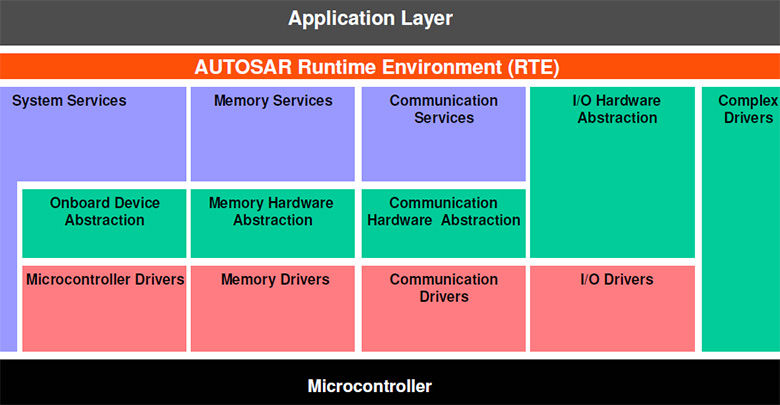
\includegraphics[width=1\textwidth]{Images/chapter2/AR_arch.jpg}
    \vspace{0.5cm}
    \caption{AUTOSAR Classic Architecture}
    \label{fig:autosar_classic_arch}
\end{figure}

However, the increasing complexity of modern automotive systems, particularly in the domains of Advanced Driver Assistance Systems (ADAS) and autonomous driving, demands computational capabilities that exceed the design limits of the Classic Platform. To address these emerging requirements, the Adaptive AUTOSAR platform was introduced. It complements the Classic Platform by providing a flexible, high-performance runtime environment for data-intensive applications and service-oriented architectures, supporting dynamic updates and high-bandwidth communication. However, the Adaptive AUTOSAR platform is not a drop-in replacement for the Classic Platform, it runs parallel to the Classic Platform with other non-AUTOSAR software modules. Rather, it will interact with these platforms and external backend systems such as road-side infrastructures, to form an integrated system. As in Figure \ref{fig:autosar_adaptive_and_classic}, CP already incorporates SOME/IP, which is also supported by AP, among other protocols.

\begin{figure}[h]
    \centering
    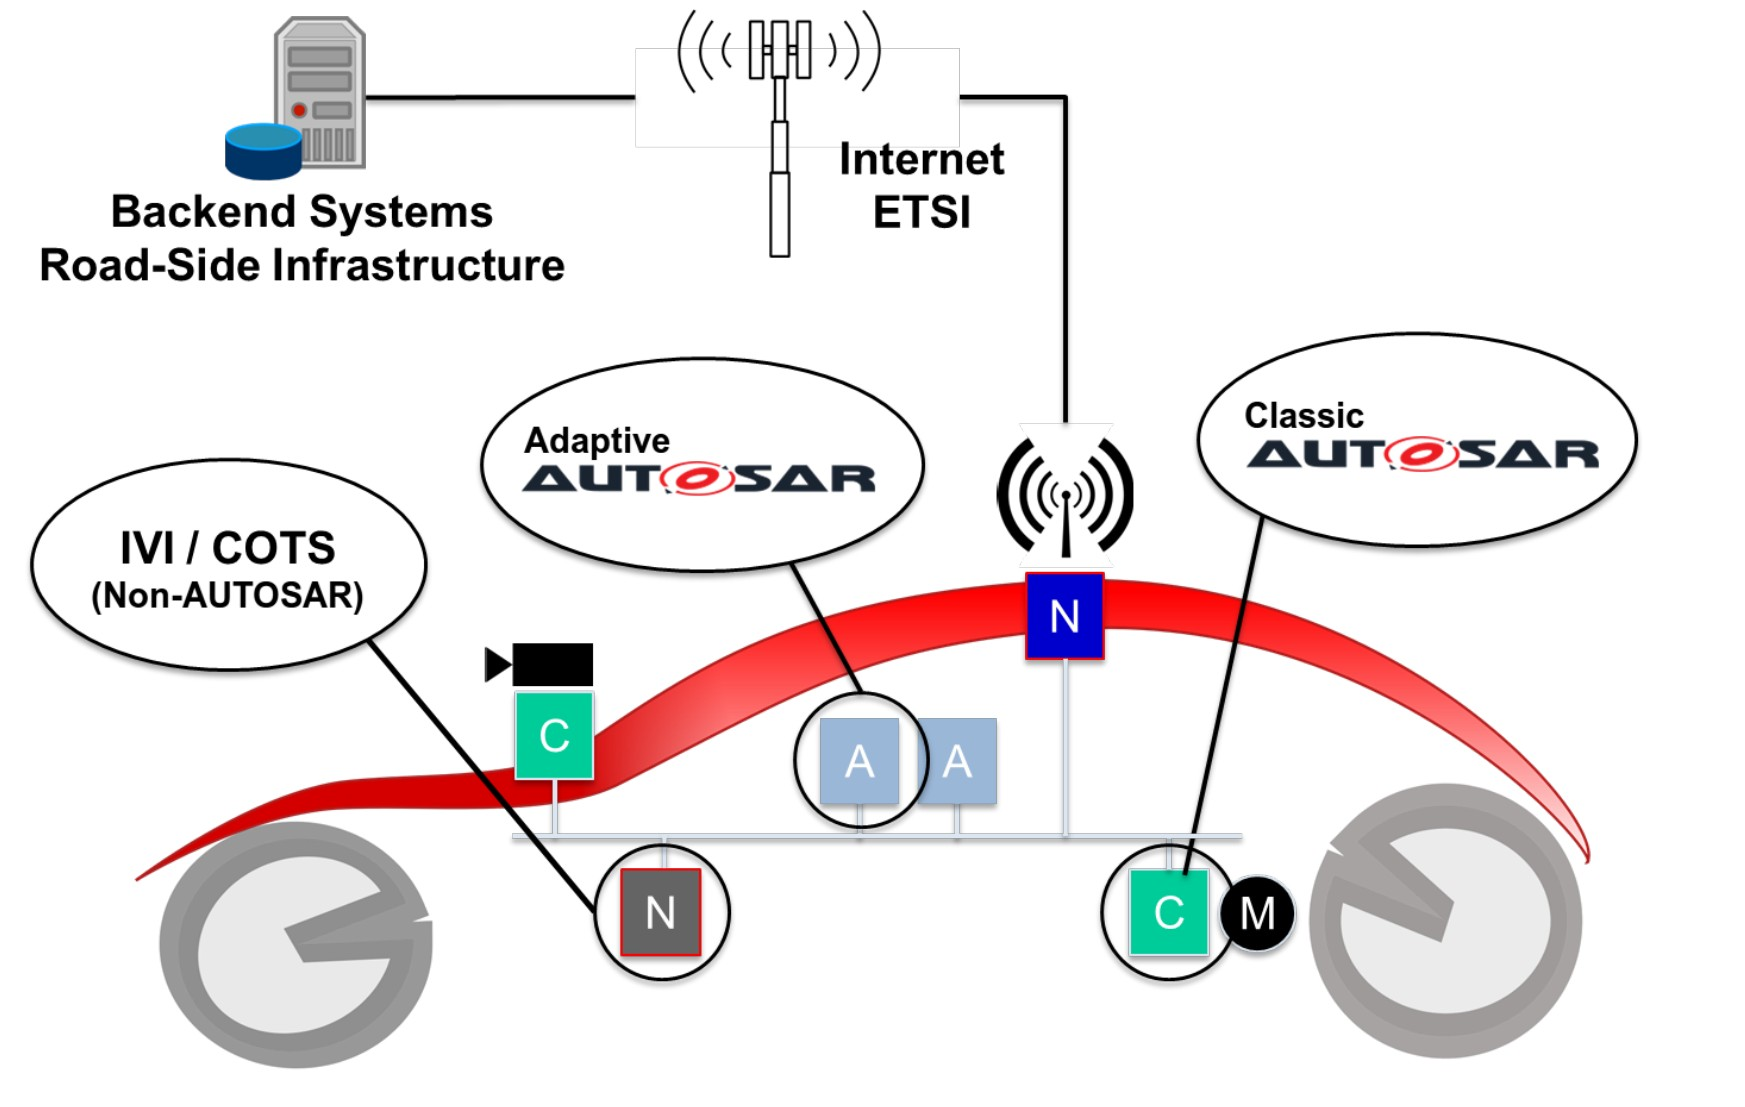
\includegraphics[width=1\textwidth]{Images/chapter2/ARandAP.jpg}
    \vspace{0.5cm}
    \caption{Exemplary deployment of different platforms \cite{autosar_platform_design}}
    \label{fig:autosar_adaptive_and_classic}
\end{figure}


The architectural designs of the Application Layer in the Adaptive Platform are based on a Service-Oriented Architecture (SOA). This allows the application to offer services to other applications and to subscribe to services provided by others. The Adaptive Platform provides a runtime environment known as the AUTOSAR Runtime for Adaptive Applications (ARA). ARA consists of a set of Functional Clusters that offer standardized services to the Adaptive Applications (AA) through a defined API.

These Functional Clusters are grouped into "Foundation" and "Services". The Foundation mainly provides platform-level functionalities such as Execution Management and Communication Management, while Services offer standard application-level capabilities. The platform runs on top of a POSIX-compliant operating system (e.g., Linux), which allows for high performance and flexibility. This layered architecture is depicted in Figure \ref{fig:autosar_adaptive_arch}, illustrating the separation between the Application, the Runtime Environment, and the underlying Operating System and Hardware.

\begin{figure}[h]
    \centering
    \includegraphics[width=1\textwidth]{Images/chapter2/AP_Arch.png}
    \vspace{0.5cm}
    \caption{Logical View of AUTOSAR Adaptive Platform Architecture \cite{autosar_platform_design}}
    \label{fig:autosar_adaptive_arch}
\end{figure}

\newpage

In the context of this project, the Adaptive Platform serves as the underlying framework for the Traffic Light Recognition System. This system utilizes the Scalable service-Oriented MiddlewarE over IP (SOME/IP) protocol and Data Distribution Service (DDS) to facilitate inter-process communication. The current implementation phase prioritizes the mechanisms of process interaction and system observability; consequently, the primary focus is placed on the Execution Management (ara::exm), Communication Management (ara::com), and Log and Trace (ara::log) functional clusters.


% \subsection{Scalable service-Oriented Middleware over IP (SOME/IP) Protocol}
% \label{sec:someip_protocol}
% \subsubsection{Service Definition}

% The Scalable service-Oriented Middleware over IP (SOME/IP) is an automotive middleware solution designed to enable efficient inter-process communication using a service-oriented architecture. Constructed on top of the Internet Protocol (IP), SOME/IP facilitates the dynamic deployment of applications by abstracting communication into defined services. A service within the SOME/IP protocol is formally defined as a logical grouping of zero or more remote procedure calls, data updates, and status properties, which are technically categorized as Methods, Events, and Fields.

% Methods represent the fundamental remote procedure calls (RPC) of the protocol. A method allows a client application (subscriber) to issue a call that is executed on the server side (provider). SOME/IP supports two primary types of methods: a "Request/Response" method, where the client waits for a reply containing the result or an error, and a "Fire \& Forget" method, where the client issues a command without expecting a response\cite[pp.~4, 15]{autosar_someip}. Events, in contrast, are specialized callback mechanisms used for data transport. They are unidirectional messages transmitted from the provider to the subscriber, typically triggered cyclically or upon a value change within the provider\cite[pp.~4, 16]{autosar_someip}.

% Fields serve to represent the status or property of a service instance. A Field is essentially a combination of up to three distinct access mechanisms: a Notifier, a Getter, and a Setter. The Notifier behaves similarly to an Event, transmitting the field's value to subscribers whenever it changes. The Getter is a method that allows a subscriber to explicitly query the current value of the field from the provider. Conversely, the Setter is a method that permits a subscriber to modify the value of the field on the provider side\cite[pp.~2, 4]{autosar_someip}. These interaction patterns form the basis of the SOME/IP communication model and are essential for automotive signal handling.

% \subsubsection{Motivation}

% The transition to Ethernet-based architectures in modern vehicles is driven by the demand for high-bandwidth applications, such as advanced infotainment and driver assistance systems. However, unlike traditional shared automotive buses (e.g., CAN), Ethernet is a switched network. This created a critical need for middleware capable of efficiently managing control data across this new medium.

% When the industry evaluated existing IT middleware standards—such as CORBA and Apache Thrift—they proved unsuitable. They were primarily designed for IT environments, lacked essential features like UDP support, and were too resource-intensive for the strict constraints of embedded Electronic Control Units (ECUs).

% To address this gap, Scalable service-Oriented Middleware over IP (SOME/IP) was developed. It provides an optimized protocol that supports CAN-like communication over Ethernet while seamlessly aligning with critical AUTOSAR concepts, such as the Client/Server and Sender/Receiver models. By fulfilling these specific automotive requirements, SOME/IP serves as the essential bridge connecting the IT/Linux domain with the Embedded/AUTOSAR domain within the vehicle network.

% % The transition toward Ethernet-based architectures in modern vehicles is driven by the increasing demand for high-bandwidth applications, such as advanced infotainment systems, driver assistance features like surround-view cameras, and the necessity for a high-speed domain backbone. While Ethernet provides a robust physical layer and the TCP/IP stack offers a proven solution for data transport, the automotive industry faced a significant challenge in identifying a suitable middleware solution capable of handling control data efficiently over this switched medium. Unlike traditional automotive buses, Ethernet is not a shared bus, necessitating a middleware that could efficiently manage unicast communication while keeping multicast and broadcast traffic to acceptable levels.

% % The primary motivation for developing Scalable service-Oriented Middleware over IP (SOME/IP) stemmed from the specific requirements of automotive communication that existing IT standards could not meet. The industry required a solution that supported CAN-like communication and MOST-like control messages but was optimized for switched Ethernet networks. An extensive evaluation of existing middleware solutions—including DCE RPC, CORBA, and Apache Thrift—revealed that these protocols were primarily designed for IT environments and were unsuitable for embedded automotive applications. These existing solutions often lacked necessary features (such as UDP support), were too resource-intensive, or required significant modification and "stripping down" to function within the constraints of automotive electronic control units (ECUs).

% % Furthermore, compatibility with the AUTOSAR standard was a critical factor in the development of SOME/IP. Existing IT solutions did not support AUTOSAR, and integrating them would have been critical and difficult to standardize. The industry needed a protocol that aligned with AUTOSAR concepts, such as the Client/Server model (Request/Response) and the Sender/Receiver model (Fire and Forget), without being restricted by the AUTOSAR license itself. SOME/IP was designed to fill this specific gap, serving as the only solution that satisfies all automotive requirements while acting as a bridge between the IT/Linux domain and the Embedded/AUTOSAR domain. Consequently, SOME/IP provides a scalable, efficient middleware solution that ensures header layouts and communication behaviors are optimized for the vehicle network.


% \subsubsection{Protocol Objectives and Architectural Role}

% \gls{SOMEIP} acts as a fundamental automotive middleware solution designed to facilitate efficient inter-process communication within the vehicle network. It provides a comprehensive specification for \glspl{RPC}, event notifications, and the underlying serialization wire format.. While initially developed to address the limitations of enterprise middleware in automotive environments, its primary architectural role today is to ensure scalability and resource efficiency across heterogeneous systems.

% A core objective of the protocol is to operate across a diverse range of hardware platforms. It scales seamlessly from small, resource-constrained electronic control units (ECUs) like cameras to complex, high-performance infotainment head units. To achieve this, the serialization protocol is designed to be linearly serialized without complex dynamic operations, ensuring it can be supported by simple tooling and run efficiently on embedded devices.

% From an architectural perspective, \gls{SOMEIP} embodies the principles of \gls{SOA} by abstracting underlying network complexity. By exposing well-defined Service Interfaces rather than raw signals, it promotes loose coupling between components. This is enforced by the \gls{SOMEIP} Service Discovery (SD) mechanism, which allows clients to dynamically detect available service instances at runtime. This shift enables the modularization of complex distributed applications, facilitating a flexible and robust vehicle network backbone that bridges the IT-centric Linux domain and the embedded \gls{AUTOSAR} domain.

% \subsubsection{Specification of \gls{SOMEIP} Message Format (Serialization)}

% The specification of \gls{SOMEIP} message format defines how communication data is structured, serialized, and transmitted between distributed components in an automotive Ethernet environment. At its core, a \gls{SOMEIP} message consists of a well-defined header followed by a payload. The header carries metadata crucial for message identification, routing, version control, and error handling, while the payload contains application-level data encoded according to strict serialization rules. These rules support a variety of data types and ensure consistency, extensibility, and backward compatibility across different versions of software and \glspl{ECU}. By standardizing both the header and payload structures, \gls{SOMEIP} enables reliable and scalable service-oriented communication in modern vehicle architectures.

% In this figure, the structure of \gls{SOMEIP} consists of two major components: \textbf{Header} and \textbf{Payload}.

% \begin{figure}[h]
%     \centering
%     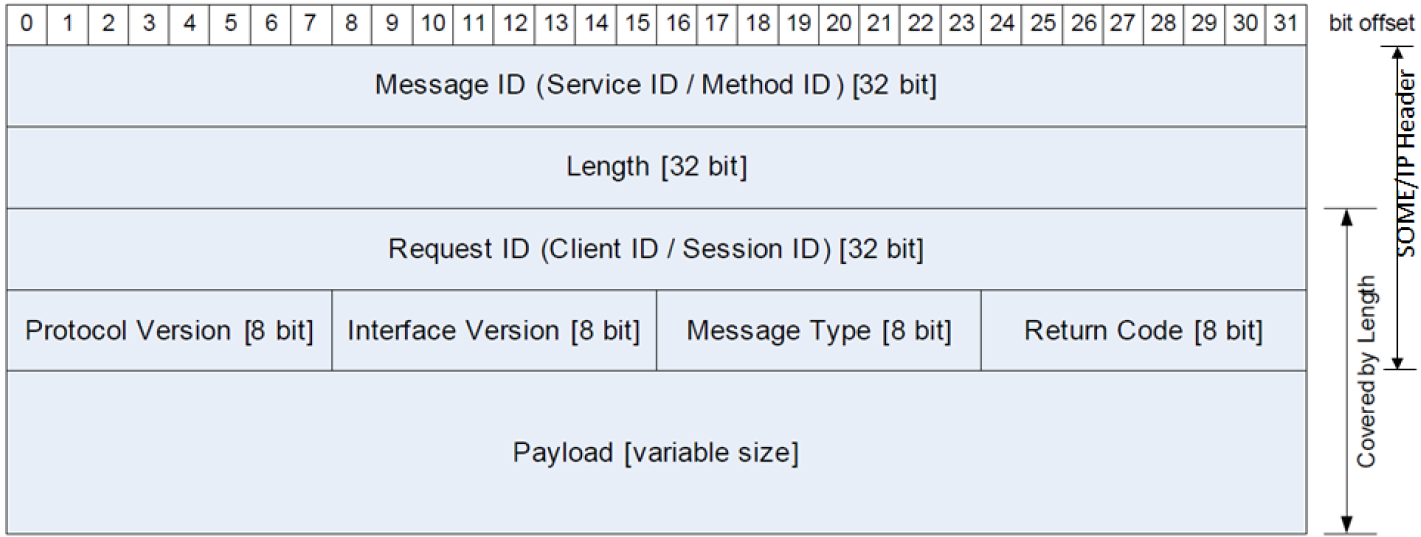
\includegraphics[width=1\textwidth]{Images/chapter2/HeaderSomeip.png}
%     \vspace{0.5cm}
%     \caption{Structure of \gls{SOMEIP} message format}
%     \label{fig:someip_structure}
% \end{figure}

% \paragraph*{Header of \gls{SOMEIP} protocol:} The header of the \gls{SOMEIP} protocol includes essential fields such as the \textbf{Message ID}, \textbf{Length}, \textbf{Client ID}, \textbf{Session ID}, \textbf{Protocol Version}, \textbf{Interface Version}, \textbf{Message Type}, and \textbf{Return Code}. These fields provide necessary metadata for identifying services, ensuring compatibility, managing sessions, and indicating the message status during communication between \glspl{ECU}.

% \textbf{Message ID [32 Bit]:} The Message ID is a 32-bit identifier used to uniquely identify either a remote procedure call (RPC) method or an event within the \gls{SOMEIP} protocol. This identifier is structured into two parts: the upper 16 bits represent the \textbf{\textit{Service ID}}, which distinguishes up to 65,536 different services, and the lower 16 bits represent the \textbf{\textit{Method ID}}, which specifies individual methods or events within that service. By convention, Method IDs in the range from \texttt{0x0000} to \texttt{0x7FFF} are reserved for RPC methods, while IDs in the range from \texttt{0x8000} to \texttt{0x8FFF} are used for events and notifications. This structured format ensures clear and scalable message identification across the entire system.

% \textbf{Length [32 Bit]:} Length field will show the length in Byte starting from Request ID/Client ID until the end of the SOME/IP message.

% \textbf{Request ID [32 Bit]}: The Request ID is a 32-bit field used to uniquely distinguish concurrent service calls between clients and servers in \gls{SOMEIP}. It is logically divided into two 16-bit segments: the \textbf{\textit{Client ID}} and the \textbf{\textit{Session ID}}. The Client ID identifies the sender of the request, allowing the receiver to differentiate among multiple clients. The Session ID is used to distinguish multiple invocations of the same method, enabling parallel or sequential tracking of communication flows. The Request ID must remain unique during the lifetime of a request-response transaction to ensure proper matching of replies.

% In some implementations, especially in large systems like a vehicle-wide network, the Request ID may be further structured to enhance uniqueness and traceability. In this extended form, the Request ID is split into three components: an 8-bit \textbf{\textit{Client ID Prefix}} (e.g., a diagnostic address or preconfigured application ID), an 8-bit \textbf{\textit{Client ID}}, and a 16-bit \textbf{\textit{Session ID}}. This structure supports globally unique identification across all \glspl{ECU} in the vehicle and facilitates more flexible configuration and routing of service calls.

% \textbf{Protocol Version [8 Bit]}: This field indicates the version of the \gls{SOMEIP} protocol used in the message. It allows systems to detect and handle incompatible changes in the protocol format. The Protocol Version only reflects the versioning of the header structure, not the payload. Currently, the standard value for this field is \texttt{0x01}. Any incompatible change in the header layout must result in an increment of this version to maintain interoperability between different protocol versions.

% \textbf{Interface Version [8 Bit]}: The Interface Version identifies the major version of the service interface and reflects changes in the structure of the payload data. A receiver uses this value to determine whether it can correctly interpret the message contents. Unlike the protocol version, which is about the header, the interface version focuses on the application-layer data structures and semantics. This field is particularly important when evolving service definitions across software updates.

% \textbf{Message Type [8 Bit]}: The Message Type field defines the nature of the message being transmitted. It specifies whether the message is a request, response, notification, or an error. This is a table shows type of message, each message corresponds to number of code 

% \textbf{Return Code [8 Bit]}: The Return Code is used to indicate the status of message processing. While it is generally set to \texttt{0x00} (E\_OK) in non-response messages, it conveys success or failure in response and error messages. For example, \texttt{0x01} indicates a generic error, \texttt{0x03} signals an unknown method, and \texttt{0x09} is used for malformed messages. This field provides a mechanism for reporting both application-level and protocol-level issues in communication.

% \newpage
% \begin{figure}[h]
%     \centering
%     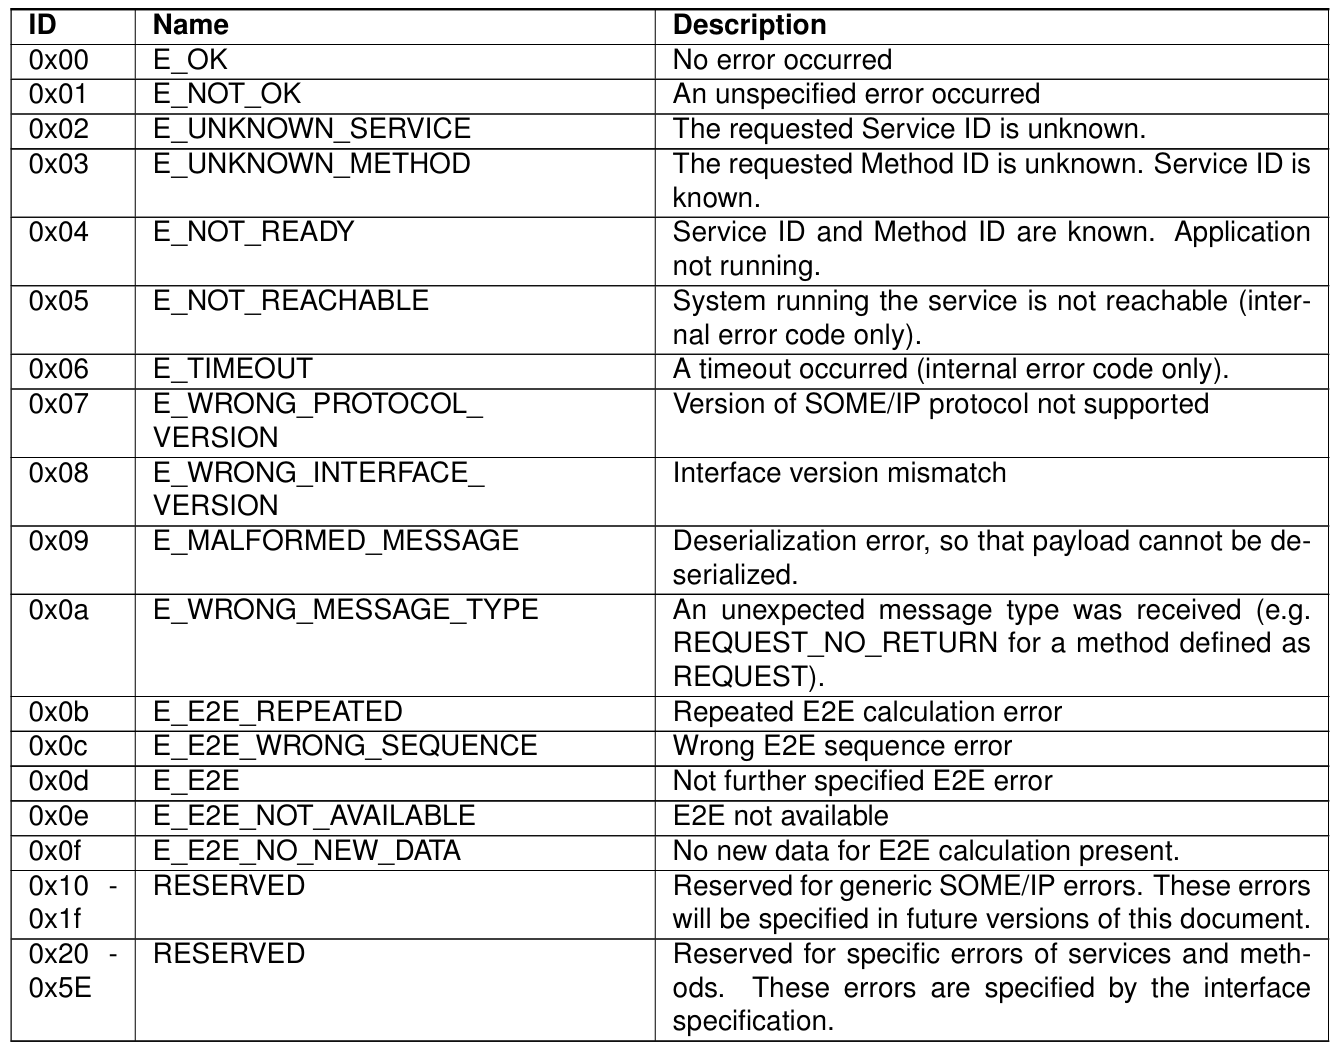
\includegraphics[width=1\textwidth]{Images/chapter2/errSomeip.png}
%     \vspace{0.5cm}
%     \caption{The table of Message Type field}
% \end{figure}
% \newpage
% \paragraph*{Payload and Serialization:}
% The \textbf{Payload} in a \gls{SOMEIP} message carries the actual data that is exchanged between a client and a server. It represents the parameters for a method call, the return values of a response, or the content of a notification/event. The payload structure is determined by the service interface definition and may consist of basic data types (e.g., integers, booleans, floats) or complex data types such as structs, arrays, strings, unions, and enumerations. Depending on the message context, the payload may be empty or contain multiple serialized arguments.

% \textbf{Serialization} refers to the process of encoding these data structures into a linear byte stream suitable for transmission over the network. The SOME/IP protocol specifies strict rules for serialization, including byte ordering (typically big-endian for header fields), memory alignment, and padding strategies. For complex types like structs, serialization closely follows in-memory layout with explicit handling of optional members and extensibility using data IDs and tags. Arrays and strings can be fixed or variable in length and often include a length field to aid deserialization. These rules ensure interoperability between different ECUs, allowing them to parse and understand messages even when optional fields or future extensions are added.

% \begin{figure}[h]
%     \centering
%     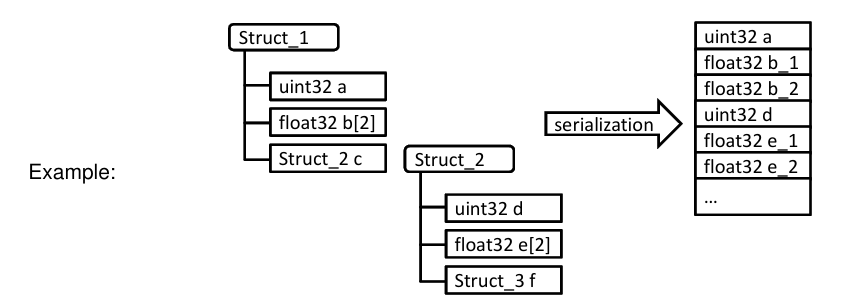
\includegraphics[width=1\textwidth]{Images/chapter2/serializationSomeip.png}
%     \vspace{0.5cm}
%     \caption{The mechanism of serialization code structure}
% \end{figure}


% Furthermore, SOME/IP supports flexible and forward-compatible serialization mechanisms through the use of tag-length-value (TLV) encoding. TLV allows new members to be added at arbitrary positions in a message, enhancing compatibility between software versions. During deserialization, unknown tags can be skipped, which prevents older receivers from crashing due to unexpected data. This extensibility is crucial in automotive systems where long product lifecycles and incremental software updates are common. This is an example of serialization of the structure code with tags.

% \newpage

% \begin{figure}[h]
%     \centering
%     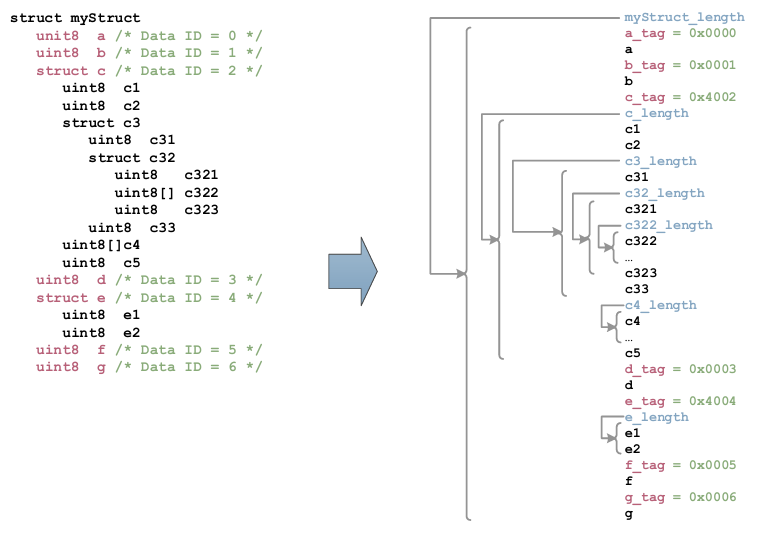
\includegraphics[width=1\textwidth]{Images/chapter2/serializationexSomeip.png}
%     \vspace{0.5cm}
%     \caption{An example of serialization of the structure code with tags}
% \end{figure}

% To sum up, the specification of the \gls{SOMEIP} message format provides a robust framework for structuring and transmitting data across distributed systems within automotive networks. By clearly defining the header fields and enforcing rigorous serialization rules for the payload, \gls{SOMEIP} ensures message consistency, interoperability, and forward compatibility. Whether handling simple method calls or complex data structures, the protocol's design supports scalable and efficient communication between heterogeneous \glspl{ECU}. This serialization standard is a key in enabling service-oriented architectures for connected and software-defined vehicles, paving the way for reliable in-vehicle communication and future-proof software integration.

% \subsubsection{Specification of \gls{SOMEIP} Protocols}

% The \gls{SOMEIP} protocol facilitates service-oriented communication through three core interaction mechanisms: \textbf{Methods}, \textbf{Events}, and \textbf{Fields}. These elements define how data and commands are exchanged between clients and servers, supporting various communication patterns ranging from synchronous remote procedure calls to asynchronous state synchronization.

% \paragraph*{Methods:}
% Methods allow a client to invoke a procedure on a server instance. \gls{SOMEIP} distinguishes between two primary types of method invocations based on whether a reply is required:

% \begin{figure}[h]
%     \centering
%     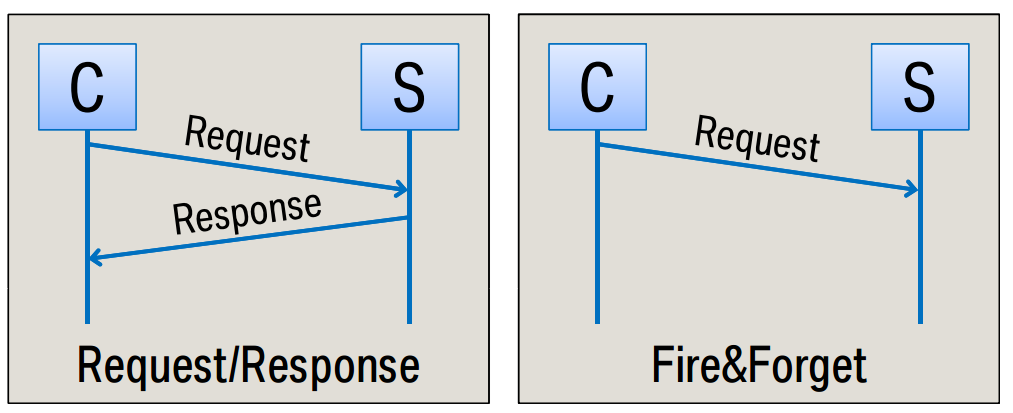
\includegraphics[width=0.8\textwidth]{Images/chapter2/MethodSomeip.png}
%     \vspace{0.5cm}
%     \caption{Methods in \gls{SOMEIP} \cite{open_alliance_someip}}
% \end{figure}

% \newpage
% \textbf{Request/Response:} This is the standard Remote Procedure Call (RPC) pattern. The client sends a \texttt{REQUEST} message (type \texttt{0x00}) and waits for a feedback. The server processes the command and returns either a \texttt{RESPONSE} message (type \texttt{0x80}) containing the result or an \texttt{ERROR} message (type \texttt{0x81}) if the operation failed. This pattern ensures transactional integrity and is equivalent to synchronous service calls in 

% \textbf{Fire \& Forget:} In this pattern, the client sends a \texttt{REQUEST\_NO\_RETURN} message (type \texttt{0x01}). The server executes the method but does not send a response, regardless of success or failure. This is useful for non-critical commands where bandwidth optimization is prioritized over confirmation, effectively decoupling the client from the server's processing time.

% \paragraph*{Events:}
% An Event represents a unidirectional, asynchronous data transmission from the server to subscribed clients. It utilizes the \texttt{NOTIFICATION} message type (\texttt{0x02}).

% Events follow the Publish/Subscribe model. A client must explicitly subscribe to an event group to receive these messages. The server triggers events based on specific logic:

% \begin{figure}[h]
%     \centering
%     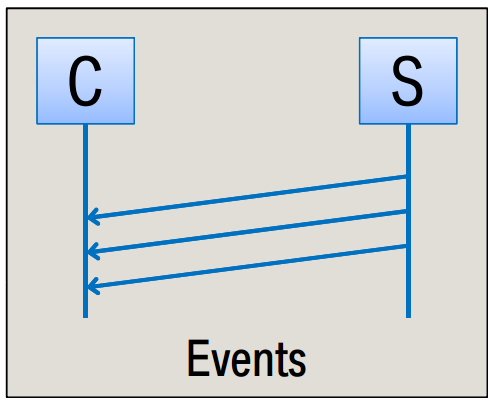
\includegraphics[width=0.4\textwidth]{Images/chapter2/EventSomeip.png}
%     \vspace{0.5cm}
%     \caption{Events in \gls{SOMEIP} \cite{open_alliance_someip}}
% \end{figure}

% \textbf{Cyclic:} Transmitted at a fixed time interval (e.g., vehicle speed sent every 100ms).

% \textbf{On Change:} Transmitted only when the value changes (e.g., a door open warning).

% \paragraph*{Fields:}
% A Field represents a status or a state variable managed by the server. Unlike a simple Event, a Field combines three distinct access mechanisms to ensure data consistency across the distributed system:

% \begin{figure}[h]
%     \centering
%     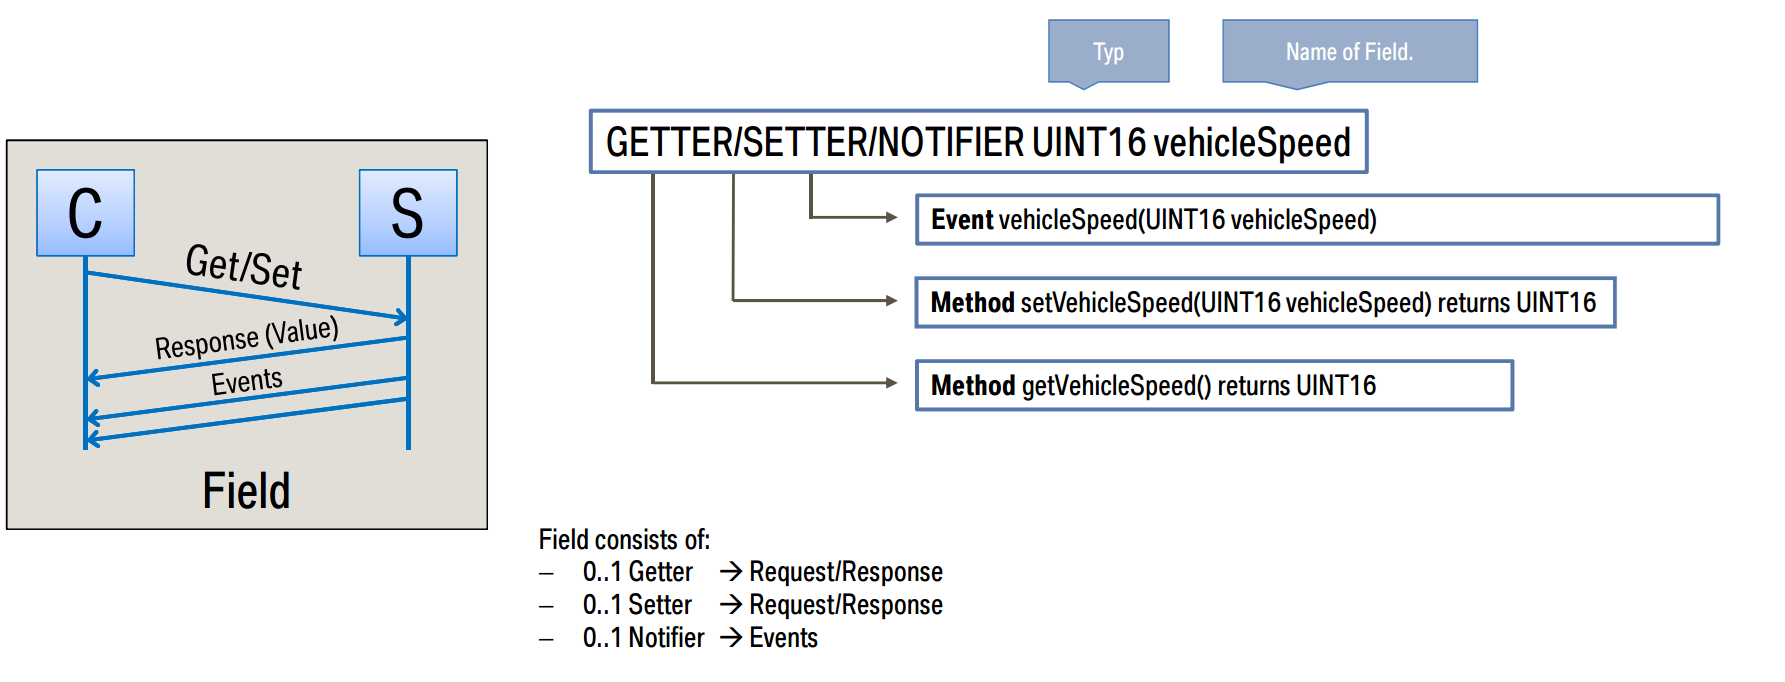
\includegraphics[width=1\textwidth]{Images/chapter2/FieldSomeip.png}
%     \vspace{0.5cm}
%     \caption{Fields in \gls{SOMEIP} \cite{open_alliance_someip}}
% \end{figure}

% \textbf{Setter:} A Request/Response method allowing a client to modify the value of the field remotely.

% \textbf{Getter:} A Request/Response method allowing a client to explicitly read the current value of the field.

% \textbf{Notifier:} An asynchronous event notification sent to subscribers whenever the field's value changes.

% \paragraph*{Comparison: Event vs. Field:}
% While both Events and Field Notifiers use asynchronous notifications to transmit data, their architectural purpose differs regarding state management:

% \textbf{Events} are best suited for momentary occurrences or streaming data where the history is less relevant than the immediate update. If a client subscribes to an Event after a transmission has occurred, it must wait for the next occurrence to receive data.

% \textbf{Fields} represent a persistent state. The inclusion of \textbf{Getter} and \textbf{Setter} methods ensures that a client can retrieve the current state immediately upon connecting, without waiting for the next change notification. Therefore, Fields are preferred when data synchronization and initial state validity are critical.

% Fields support both pull-based (getter/setter) and push-based (notifier) communication styles. This concept can be mapped to shared variables or observable state in enterprise software where consistent data synchronization is required.

% \paragraph*{Error Handling:}

% In addition to the three communication elements, \gls{SOMEIP} provides a robust error handling mechanism. Every message includes a \texttt{Return Code} field that indicates whether the operation succeeded (\texttt{0x00} for E\_OK) or failed (e.g., \texttt{0x03} for E\_UNKNOWN\_METHOD).

% When additional diagnostic information is needed, servers can send a dedicated \texttt{ERROR} message (\texttt{0x81}), which may include structured error payloads such as exception types or debug messages. This supports fault detection, debugging, and graceful degradation—critical concerns in enterprise-grade software systems.

% Moreover, protocol-level validations such as version mismatch detection, unexpected message checks, and session management are built-in, ensuring communication resilience and system integrity.

% \newpage
% \begin{figure}[h]
%     \centering
%     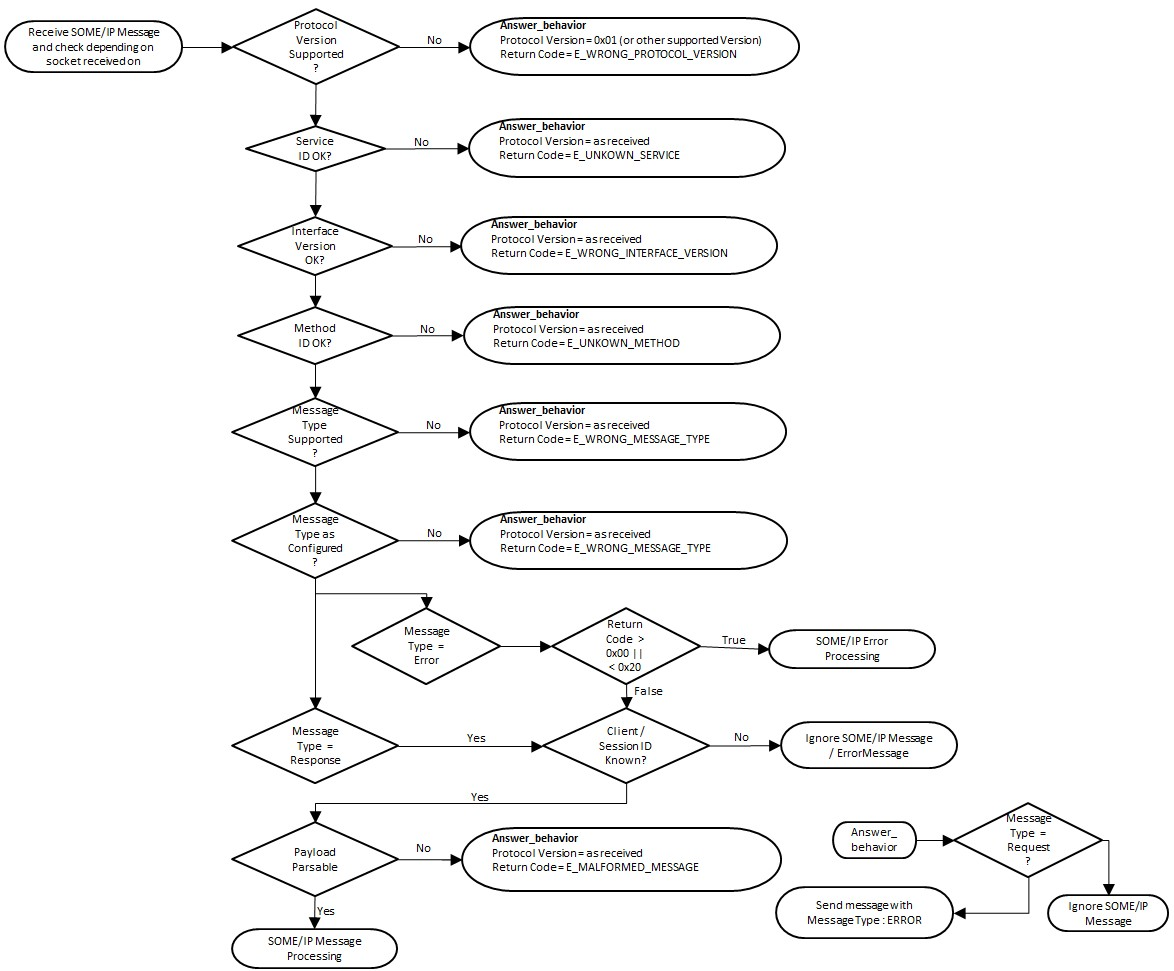
\includegraphics[width=1\textwidth]{Images/chapter2/ErrorHandlerSomeip.jpg}
%     \vspace{0.5cm}
%     \caption{Error handling in \gls{SOMEIP} \cite{open_alliance_someip}}
% \end{figure}


% The specification of \gls{SOMEIP} communication through its Method, Event, and Field elements, along with a comprehensive error handling strategy, demonstrates a well-structured approach to designing scalable and interoperable distributed systems. These mechanisms are not only tailored to meet the stringent real-time and safety requirements of automotive applications, but they also reflect well practices found in enterprise software architecture, such as modularity, service encapsulation, event-driven design, and fault tolerance. Understanding and applying these communication models facilitates the development of robust service-oriented systems that align with modern software engineering principles.

% \subsubsection{SOME/IP-SD (SOME/IP Service Discovery)}

% SOME/IP Service Discovery (SOME/IP-SD) is the dedicated protocol extension used to manage the availability of service instances and the dynamic establishment of communication paths within an automotive Ethernet network. While standard IT service discovery mechanisms focus primarily on locating a service, SOME/IP-SD is optimized for automotive requirements, focusing heavily on service availability (determining if a service is ready to be used) and the management of Publish/Subscribe relationships for event handling. The protocol is designed to run on embedded devices with limited overhead, allowing multiple service interactions to be encoded within a single packet. SOME/IP-SD messages are transported over UDP (and less commonly TCP) using the standard SOME/IP header, but they utilize a fixed Message ID of 0xFFFF 8100 to distinguish them from standard application RPC messages.
% The architecture of a SOME/IP-SD message consists of a specific payload layout that follows the standard SOME/IP header. This payload is organized into Flags, an Entries Array, and an Options Array. The Entries Array contains the core commands, such as finding services or subscribing to events, while the Options Array carries variable data, such as IP addresses, port numbers, or configuration strings, which are referenced by the entries using indices. A vital component of the SD header is the Flag field, specifically the Reboot Flag. This flag allows ECUs to detect if a communication partner has restarted. The Session ID in the header increments with every transmission; if a receiver detects that the Session ID has reset or that the Reboot Flag has been toggled, it knows the partner ECU has rebooted and can re-initialize subscriptions or discard stale state data.

% \begin{figure}[h]
%     \centering
%     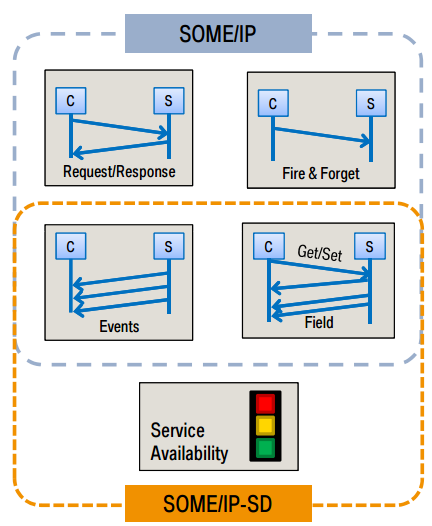
\includegraphics[width=0.5\linewidth]{Images//chapter2/someip_sd.png}
%     \vspace{0.5cm}
%     \caption{SOME/IP Service Discovery \cite{open_alliance_someip}}
%     \label{fig:someip_sd}
% \end{figure}

% \paragraph{Service Discovery Mechanisms:} There are 2 Service Discovery Mechanism: 

% \textbf{Offer and Find:} The primary function of SOME/IP-SD is to match Clients (service consumers) with Servers (service providers). The protocol utilizes specific entry types to achieve this: \texttt{OfferService} and \texttt{FindService}. When a Server ECU starts up and a service instance becomes available, it enters an "Initial Wait Phase" followed by a "Repetition Phase," where it broadcasts \texttt{OfferService} entries (typically via Multicast) to announce its presence to the network. If a Client ECU requires a service that it has not yet seen offered, it sends a FindService entry. Upon receiving a Find message, the Server responds with a unicast \texttt{OfferService} to inform the specific Client that the service is available. These entries contain a Time-To-Live (TTL) field; a non-zero TTL indicates the service is valid for a specific duration (e.g., 3 seconds), whereas a TTL of zero represents a \texttt{StopOfferService} message, informing the network that the service is no longer available.

% \begin{figure}[h]
%     \centering
%     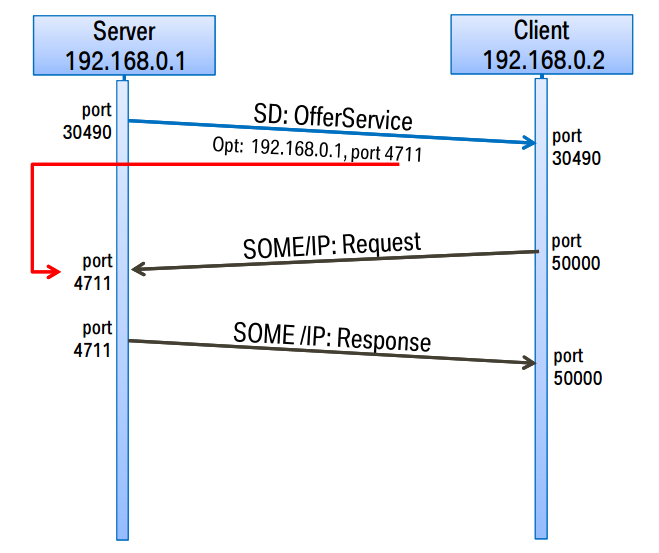
\includegraphics[width=0.5\linewidth]{Images//chapter2/someip_sd_offerandfind.png}
%     \vspace{0.5cm}
%     \caption{SOME/IP-SD Offer and Find Mechanism \cite{open_alliance_someip}}
%     \label{fig:someip-sd/findoffer}
% \end{figure}
% \newpage
% \textbf{Publish/Subscribe Management:} Beyond simple discovery, SOME/IP-SD manages the dynamic routing of events through a Publish/Subscribe mechanism. This ensures that the network is not flooded with event messages unless a Client explicitly requires them. This is handled through specific entry types: SubscribeEventgroup and SubscribeEventgroupAck. When a Client determines a service is available (via an \texttt{OfferService}), it sends a \texttt{SubscribeEventgroup} entry to the Server to request specific data streams. The Server validates this request and responds with a \texttt{SubscribeEventgroupAck} (Acknowledgement) if successful, or a \texttt{SubscribeEventgroupNack} (Negative Acknowledgement) if the request fails. Only after this handshake does the Server begin transmitting the actual event data via standard SOME/IP notification messages. 

% \begin{figure}[h]
%     \centering
%     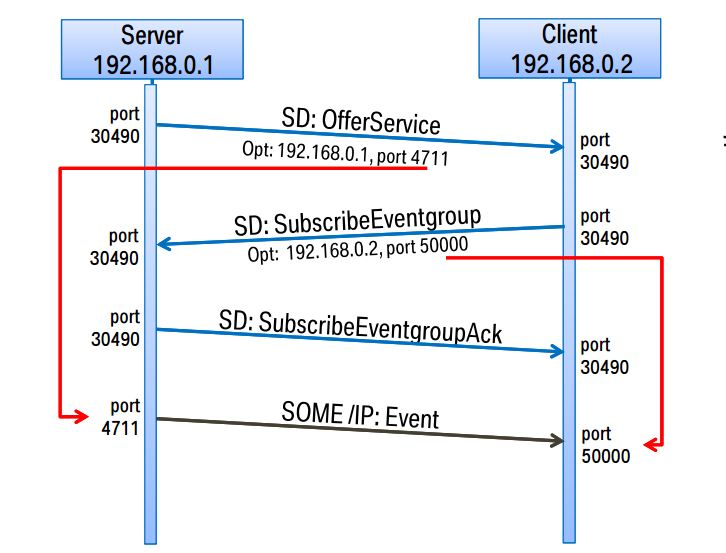
\includegraphics[width=0.5\linewidth]{Images//chapter2/someip_sdpubsub.png}
%     \vspace{0.5cm}
%     \caption{SOME/IP-SD Publish/Subscribe Mechanism \cite{open_alliance_someip}}
%     \label{fig:enter-label/pubsub}
% \end{figure}

% To link the abstract discovery of a service to the physical network parameters required to connect to it, SOME/IP-SD uses Endpoint Options. An SD Entry (like an Offer or Subscribe) does not contain the IP address or port itself; instead, it points to an Option in the Options Array. For example, an IPv4 Endpoint Option contains the IP address, the transport protocol (UDP or TCP), and the Port Number where the service can be reached. For multicast events, a Multicast Option is used by the Server in the \texttt{SubscribeEventgroupAck} to tell the Client which Multicast IP and Port to listen to for incoming events. This separation allows for efficient packing, where multiple entries can share the same endpoint options within a single message.

% \begin{figure}[h]
%     \centering
%     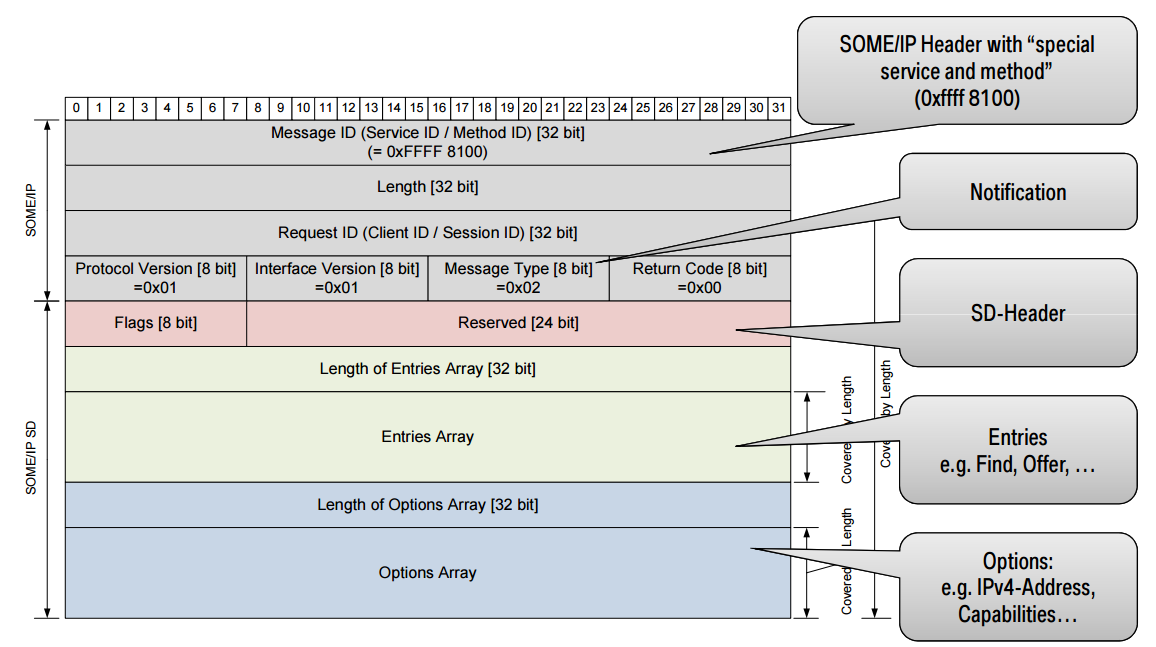
\includegraphics[width=1\linewidth]{Images//chapter2/someip_sdheader.png}
%     \vspace{0.5cm}
%     \caption{SOMEIP/SD Header \cite{open_alliance_someip}}
%     \label{fig:Someip-sdheader}
% \end{figure}
% \newpage
% \subsubsection{SOME/IP Transport Layer Bindings}

% The SOME/IP protocol is designed to operate independently of the underlying transport layer, primarily utilizing User Datagram Protocol (UDP) and Transmission Control Protocol (TCP) to transmit messages over IP-based automotive networks. The selection of the specific transport protocol is critical as it dictates the reliability, latency, and payload capacity of the communication. While UDP offers a lightweight, connectionless model suitable for frequent, small messages, TCP provides a robust, connection-oriented channel for larger data streams. Additionally, to bridge the gap between the limitations of UDP and the need to transport large data packets without the overhead of TCP, the SOME/IP Transport Protocol (SOME/IP-TP) was developed to allow for segmentation over UDP.

% \textbf{UDP Binding (User Datagram Protocol)}

% The UDP binding is the most fundamental mode of transport for SOME/IP, achieved by encapsulating SOME/IP messages directly within UDP packets. It is a connectionless protocol, meaning no handshake is required before data transmission begins. A client and server typically use a single unicast UDP connection for all methods and events configured for UDP communication, and a separate multicast connection for multicast events. Due to the nature of UDP and the standard Maximum Transmission Unit (MTU) of Ethernet frames, the payload of a SOME/IP message transmitted via UDP is strictly limited to between 0 and 1400 bytes to prevent IP fragmentation and ensure protocol stability.

% UDP is the preferred choice for automotive applications requiring very low latency (typically under 100ms) and fast reaction times. It is ideal for "Fire \& Forget" communication or cyclic data transmission—such as vehicle speed or engine RPM—where the occasional loss of a packet is acceptable because the next cycle will update the information shortly. The protocol supports "Maybe" reliability semantics, meaning the application must be designed to handle scenarios where a message might not reach its destination. Furthermore, UDP is the required transport mechanism for multicast communication, where a single publisher sends notifications to multiple subscribers simultaneously .

% The primary drawback of the standard UDP binding is the strict payload limitation; it cannot natively transport messages larger than 1400 bytes. Additionally, because it lacks the robustness features of TCP, it does not guarantee delivery, order, or protection against duplication. If a packet is lost in the network, it is not automatically retransmitted by the transport layer, forcing the application layer to handle error scenarios or timeouts.


% \textbf{TCP Binding (Transmission Control Protocol)}

% The TCP binding provides a reliable, connection-oriented channel for SOME/IP messages. Unlike UDP, TCP supports the segmentation of payloads, allowing for significantly larger SOME/IP messages that far exceed the 1400-byte limit of UDP. The connection is managed actively: the client is responsible for opening the TCP connection when the first method call or notification is required and must re-establish it if it fails. To mitigate latency issues often associated with TCP, the protocol specification recommends disabling Nagle’s algorithm (\texttt{TCP\_NODELAY}). To assist testing tools in identifying message boundaries within the continuous TCP stream, "Magic Cookie" messages may be inserted into the stream at regular intervals.

% TCP is utilized when "Exactly Once" reliability is required, ensuring that messages arrive correctly, in order, and without duplication. It is the optimal choice for transmitting large chunks of data—such as map data, diagnostic logs, or complex data structures—where the payload exceeds 1400 bytes and the strict latency requirements of control loops are not the primary constraint.

% The robustness of TCP comes at the cost of higher overhead and latency compared to UDP. The management of the connection adds complexity; the system must handle opening, closing, and monitoring the connection state. Furthermore, TCP does not support multicast; it is strictly a unicast, point-to-point protocol. If the server closes the connection unexpectedly, it can lead to synchronization issues where the client attempts to immediately re-establish the link.


% \textbf{SOME/IP-TP (Transport Protocol)}

% SOME/IP-TP is not a separate transport layer but a protocol extension applied on top of UDP to enable the segmentation of large messages that would otherwise require TCP. When a SOME/IP message is too large for a single UDP packet, it is split into smaller "segments". These segments utilize a specific Message Type (setting the TP-Flag to 1) and insert a TP-Header immediately after the standard SOME/IP header. This TP-Header contains an Offset field (indicating where in the original message the current segment belongs) and a More Segments Flag (indicating if more data follows). The receiver is responsible for collecting these segments and reassembling the original message based on the Request ID (Client ID and Session ID).

% The primary use case for SOME/IP-TP is transmitting large data payloads (>1400 bytes) in scenarios where the hard latency requirements prohibit the use of TCP. It allows engineers to maintain the speed and connectionless nature of UDP while bypassing its size limitations. It is often used for transmitting large sensor data or camera images where real-time delivery is prioritized over the absolute guarantee of delivery provided by TCP.

% SOME/IP-TP introduces significant complexity to the receiving stack. The receiver must manage reassembly buffers and handle various error cases, such as overlapping, duplicated, or missing segments. Crucially, SOME/IP-TP does not support the reordering of segments; if a segment is lost or arrives out of order in a way the buffer cannot handle, the entire assembly process for that message is canceled. Furthermore, the payload of all segments (except the last one) must be a multiple of 16 bytes to ensure alignment.


% \begin{table}[h!]
% \centering
% \renewcommand{\arraystretch}{1.5} % Adjusts row height for better readability
% \begin{tabularx}{\textwidth}{|l|X|X|X|}
% \hline
% \textbf{Feature} & \textbf{UDP Binding} & \textbf{TCP Binding} & \textbf{SOME/IP-TP} \\ \hline
% \textbf{Definition} & 
% User Datagram Protocol; a connectionless, lightweight transport protocol. & 
% Transmission Control Protocol; a connection-oriented, reliable protocol. & 
% Transport Protocol; a protocol extension applied on top of UDP to enable segmentation of large messages. \\ \hline
% \textbf{Payload Capacity} & 
% Strictly limited to 0--1400 bytes to avoid IP fragmentation. & 
% Supports large payloads (stream-based) significantly larger than 1400 bytes. & 
% Supports large payloads ($>1400$ bytes) by segmenting them into smaller packets fitting the MTU. \\ \hline
% \textbf{Reliability} & 
% ``Maybe'' reliability; messages might reach the partner, but loss, duplication, or reordering is handled by the application. & 
% ``Exactly Once'' reliability; handles packet loss, reordering, and duplication automatically. & 
% Dependent on UDP; strictly does not support reordering of segments. If a segment is missing, reassembly is canceled [8]. \\ \hline
% \textbf{Latency} & 
% Very low latency; suitable for requirements $<100$ms. & 
% Higher latency due to connection overhead and reliability mechanisms (retransmissions). & 
% Lower latency than TCP; designed for large data with hard latency requirements. \\ \hline
% \textbf{Connection Management} & 
% Connectionless; no handshake required. & 
% Active connection management required (Open/Close); Client initiates connection. & 
% Connectionless (rides on UDP); requires Session Handling (Session ID) to track segments. \\ \hline
% \textbf{Multicast Support} & 
% Supported; required for multicast events. & 
% Not supported; Unicast only. & 
% Supported (as it operates over UDP). \\ \hline
% \textbf{Primary Use-Case} & 
% Cyclic data (e.g., vehicle speed), small events, ``Fire \& Forget'' communication. & 
% Large data chunks (e.g., map data, diagnostics) where no hard latency limit exists. & 
% Large data transmission (e.g., sensor fusion data) where TCP latency is unacceptable. \\ \hline
% \end{tabularx}
% \caption{Comparison of SOME/IP Transport Layer Bindings}
% \label{tab:someip_transport_comparison}
% \end{table}


\subsection{Scalable service-Oriented Middleware over IP (SOME/IP) Protocol}
\label{sec:someip_protocol}

Scalable service-Oriented Middleware over IP (SOME/IP) is an automotive middleware protocol designed for service-oriented communication over Ethernet. It was introduced to support the transition from signal-based in-vehicle networks, such as CAN and LIN, toward IP-based communication required by modern infotainment, ADAS, and software-defined vehicle architectures. Unlike traditional bus communication, Ethernet is switched and packet-based; therefore, applications require middleware that can describe services, discover providers dynamically, serialize data consistently, and transport messages efficiently between distributed ECUs.

Within Adaptive AUTOSAR, SOME/IP is one of the communication bindings used by Communication Management (\texttt{ara::com}). Its main role is to expose application functionality through well-defined service interfaces rather than direct signal access. A SOME/IP service is composed of three main interaction elements: {Methods}, {Events}, and {Fields}. Methods implement remote procedure calls between a client and a provider. They can follow a request/response pattern, where the client waits for a result, or a fire-and-forget pattern, where no response is expected. Events implement unidirectional data transmission from a provider to subscribed clients, usually triggered cyclically or when a value changes. Fields represent service state and combine getter, setter, and notifier mechanisms, allowing clients to read, modify, or subscribe to state changes \cite{autosar_someip}.

\subsubsection{SOME/IP Message Format and Serialization}

A SOME/IP message consists of a fixed header followed by an application payload. The header contains the information required to identify the service, route the message, distinguish concurrent calls, verify compatibility, and report errors. Figure~\ref{fig:someip_structure} shows the general structure of a SOME/IP message.

\begin{figure}[h]
    \centering
    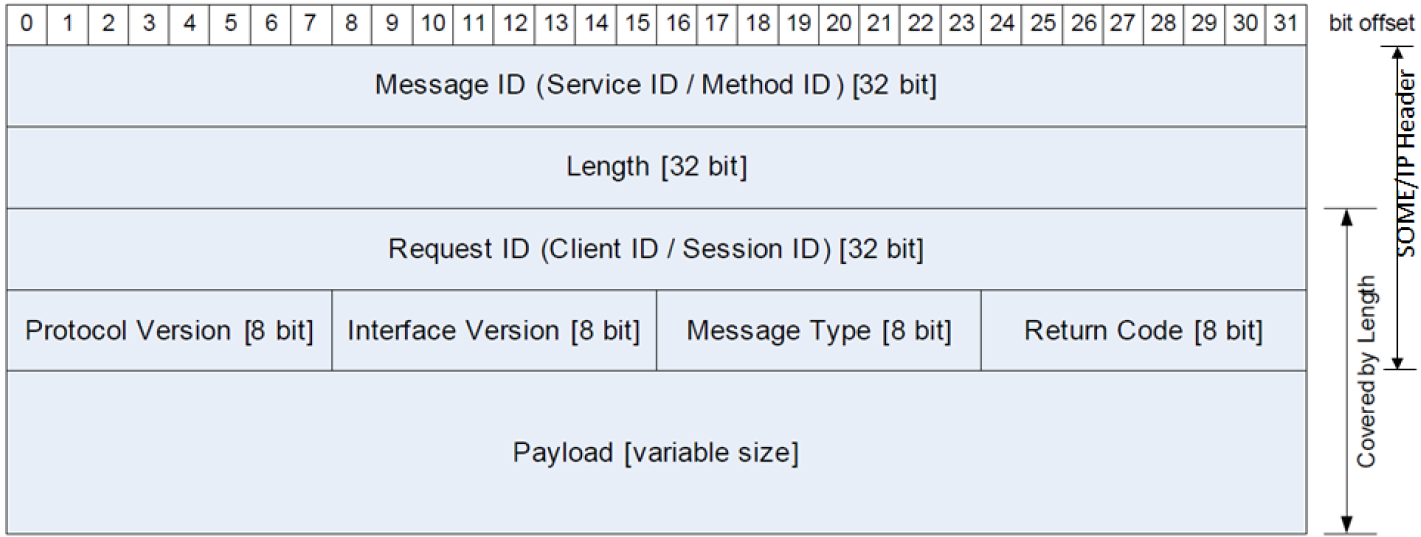
\includegraphics[width=1\textwidth]{Images/chapter2/HeaderSomeip.png}
    \vspace{0.5cm}
    \caption{Structure of \gls{SOMEIP} message format}
    \label{fig:someip_structure}
\end{figure}

The most important header field is the {Message ID}, which is divided into a Service ID and a Method/Event ID. This allows the receiver to identify which service and operation the message belongs to. The {Length} field defines the size of the remaining SOME/IP message, while the {Request ID} combines Client ID and Session ID to match requests with responses. The {Protocol Version} and {Interface Version} fields support compatibility checks between different protocol or service-interface versions. The {Message Type} indicates whether the message is a request, response, notification, or error, and the {Return Code} reports the processing result, such as successful execution or an unknown method.

The payload carries the actual application data, such as method parameters, return values, or event content. SOME/IP defines serialization rules to convert structured data into a linear byte stream suitable for network transmission. These rules cover primitive data types, structures, arrays, strings, unions, and optional extensions. Consistent serialization is essential because ECUs from different suppliers must interpret the same message layout correctly. In addition, SOME/IP supports extensible serialization mechanisms such as tag-length-value (TLV), which allow future members to be added while older receivers can skip unknown fields. This improves long-term compatibility in vehicle software platforms.

\subsubsection{SOME/IP Communication Patterns}

SOME/IP supports several communication patterns that map directly to service-oriented design. The first pattern is {request/response}, where a client sends a request and the provider returns either a response or an error. This pattern is suitable for service operations that require confirmation, such as querying a configuration value or requesting a diagnostic operation. The second pattern is \textbf{fire-and-forget}, where the client sends a request without expecting a response. This is useful for lightweight commands where confirmation is not required.

\begin{figure}[h]
    \centering
    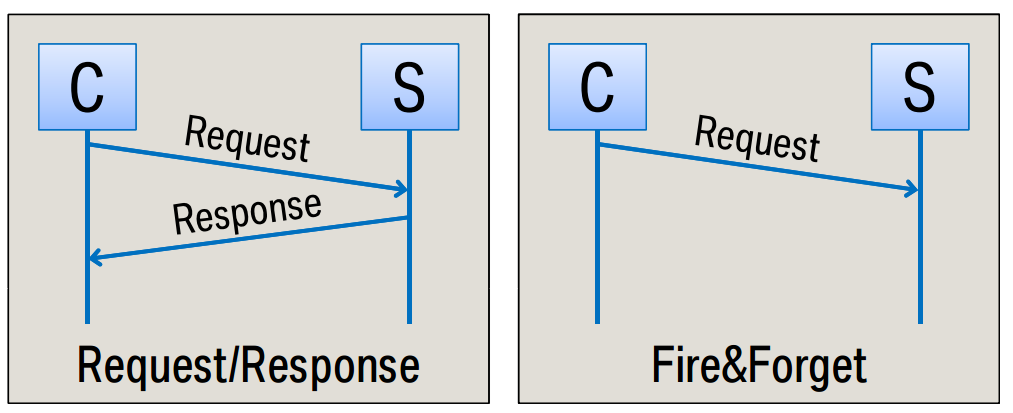
\includegraphics[width=0.8\textwidth]{Images/chapter2/MethodSomeip.png}
    \vspace{0.5cm}
    \caption{Methods in \gls{SOMEIP} \cite{open_alliance_someip}}
\end{figure}

The third pattern is {event notification}. Events follow a publish/subscribe model: a provider publishes notifications, and clients receive them only after subscribing to the relevant event group. Events may be cyclic, such as periodically transmitted vehicle speed, or on-change, such as a door-open state update. Fields extend the event concept by representing persistent service state. A field may provide a getter to read the current value, a setter to modify the value, and a notifier to inform subscribers when the value changes. Thus, events are suitable for streaming or momentary updates, while fields are suitable for state synchronization.

\begin{figure}[h]
    \centering
    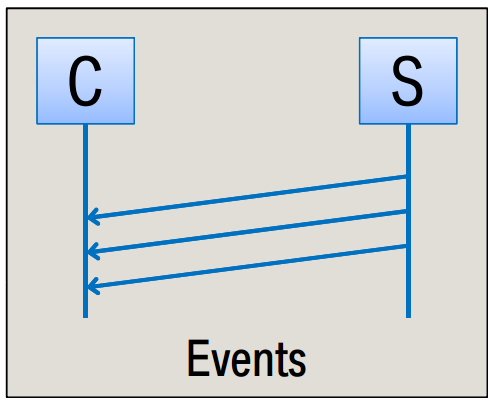
\includegraphics[width=0.45\textwidth]{Images/chapter2/EventSomeip.png}
    \vspace{0.5cm}
    \caption{Events in \gls{SOMEIP} \cite{open_alliance_someip}}
\end{figure}

Error handling is integrated into the protocol through the Return Code field and dedicated ERROR messages. For example, a provider may return an error if a method is unknown, a message is malformed, or an interface version is incompatible. These mechanisms help applications detect communication faults and handle them in a controlled manner.

\subsubsection{SOME/IP Service Discovery}

SOME/IP Service Discovery (SOME/IP-SD) manages the dynamic availability of service instances in an Ethernet network. Instead of hard-coding all communication partners, providers announce available services and clients search for the services they require. This supports the dynamic service-oriented behavior expected in Adaptive AUTOSAR systems.

\begin{figure}[h]
    \centering
    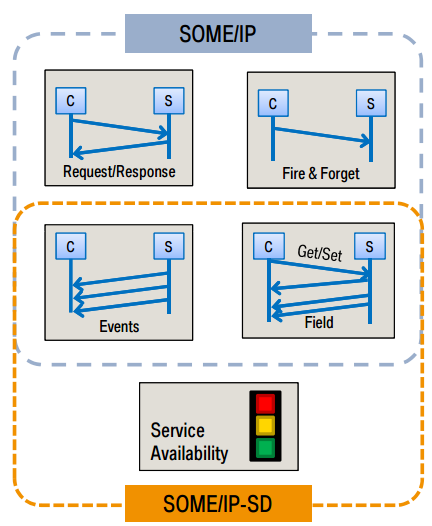
\includegraphics[width=0.5\linewidth]{Images//chapter2/someip_sd.png}
    \vspace{0.5cm}
    \caption{SOME/IP Service Discovery \cite{open_alliance_someip}}
    \label{fig:someip_sd}
\end{figure}

The basic discovery mechanism is based on \texttt{OfferService} and \texttt{FindService}. When a provider becomes available, it sends \texttt{OfferService} messages to announce the service instance. If a client needs a service that has not yet been offered, it sends a \texttt{FindService} message. The Time-To-Live (TTL) value in these messages indicates how long the service information remains valid; a TTL of zero indicates that the service is no longer available.

For event-based communication, SOME/IP-SD also manages subscriptions. After discovering a service, a client sends a \texttt{SubscribeEventgroup} request to receive selected events. The provider replies with \texttt{SubscribeEventgroupAck} or \texttt{SubscribeEventgroupNack}. Only after a successful subscription does the provider send event notifications to the client. Endpoint Options are used to connect abstract service information to concrete network parameters such as IP address, transport protocol, and port number. This separation allows service discovery to remain compact while still providing the information required for runtime communication.

\subsubsection{SOME/IP Transport Layer Bindings}

SOME/IP can be transported using UDP, TCP, or SOME/IP Transport Protocol (SOME/IP-TP). The choice depends on payload size, latency requirements, and reliability expectations. {UDP} is lightweight and connectionless, making it suitable for small, frequent, low-latency messages such as cyclic signals or fire-and-forget communication. It also supports multicast, which is required for many event notification scenarios. However, standard UDP binding is limited by the Ethernet MTU, so payloads are typically restricted to about 1400 bytes, and delivery is not guaranteed.

{TCP} provides reliable, ordered, connection-oriented transmission and can carry larger payloads. It is appropriate for data where correctness is more important than minimum latency, such as diagnostic information or larger configuration data. The trade-off is higher overhead, connection management complexity, and no multicast support.

{SOME/IP-TP} is a protocol extension over UDP that enables segmentation of large SOME/IP messages. It allows large payloads to be split into smaller UDP-compatible segments and reassembled by the receiver. This is useful when large data must be transported with lower latency than TCP. However, it increases receiver complexity because missing, duplicated, or out-of-order segments must be handled carefully.

\begin{table}[h!]
\centering
\renewcommand{\arraystretch}{1.3}
\begin{tabularx}{\textwidth}{|l|X|X|X|}
\hline
\textbf{Feature} & \textbf{UDP Binding} & \textbf{TCP Binding} & \textbf{SOME/IP-TP} \\ \hline
\textbf{Main property} & Lightweight and connectionless. & Reliable and connection-oriented. & Segmentation extension over UDP. \\ \hline
\textbf{Payload size} & Small payloads, typically up to about 1400 bytes. & Large payloads over a stream connection. & Large payloads split into UDP segments. \\ \hline
\textbf{Reliability} & Best-effort; loss is handled by the application. & Reliable, ordered delivery. & Depends on UDP; reassembly fails if required segments are missing. \\ \hline
\textbf{Typical use case} & Small cyclic data, events, multicast notifications. & Diagnostics, configuration data, larger reliable transfers. & Large low-latency data where TCP overhead is undesirable. \\ \hline
\end{tabularx}
\caption{Comparison of SOME/IP Transport Layer Bindings}
\label{tab:someip_transport_comparison}
\end{table}

In summary, SOME/IP provides a service-oriented middleware layer for Ethernet-based automotive systems. Its service model, message format, discovery mechanism, and transport bindings allow Adaptive AUTOSAR applications to communicate in a modular and scalable way. Although the final prototype in this project uses DDS for the implemented data path, SOME/IP remains important background knowledge because it is a major communication technology supported by Adaptive AUTOSAR and is widely used in service-oriented automotive architectures.

\subsection{Data Distribution Service (DDS)}

The ongoing transformation of the automotive industry toward Software-Defined Vehicles (SDVs) and high-performance computing platforms necessitates a fundamental paradigm shift in in-vehicle communication architectures. As Advanced Driver Assistance Systems (ADAS) and autonomous driving frameworks continue to evolve in complexity, the constraints of static, signal-based network topologies---such as the Controller Area Network (CAN) and the Local Interconnect Network (LIN)---become increasingly apparent. The AUTOSAR Adaptive Platform directly addresses these limitations by enforcing a Service-Oriented Architecture (SOA), which utilizes modern middleware solutions to decouple software application components from the underlying hardware and network topology. Within this architectural paradigm, the Data Distribution Service (DDS) operates as a paramount network binding protocol, offering a highly scalable, real-time, and strictly data-centric communication layer. DDS delivers the rigorous temporal determinism required by safety-critical automotive applications, while simultaneously affording the dynamic structural flexibility necessary for complex, distributed machine learning pipelines, sensor fusion networks, and high-bandwidth telemetry systems.

\subsubsection{Service Definition}

Following the specification of Data Distribution Service (DDS) protocol in Adaptive AUTOSAR~\cite{autosar_dds}, DDS is a comprehensive, open international machine-to-machine middleware standard developed, governed, and maintained by the Object Management Group (OMG). Functioning as a data-centric communication protocol, DDS abstracts the complexities of the underlying operating system, the network transport layer, and low-level data serialization formats. This abstraction layer enables seamless, distributed software application communications across highly heterogeneous hardware architectures and diverse programming languages, bridging the gap between embedded microcontrollers and high-performance computing clusters.

At its foundational core, the DDS standard establishes the concept of a virtual ``Global Data Space.'' Within this logical construct, distributed applications can asynchronously share information without requiring direct point-to-point connections. Participating nodes within the network do not exchange opaque, unstructured messages; instead, they read and write strongly typed data-objects. These data-objects are uniquely addressed by an application-defined name, known as a ``Topic,'' combined with a specific cryptographic or logical ``Key'' that identifies discrete, localized instances of that data. The DDS specification rigorously defines both the Application Programming Interfaces (APIs) and the underlying communication semantics required to facilitate this highly structured exchange between data providers and data consumers.

\begin{figure}[h]
    \centering
    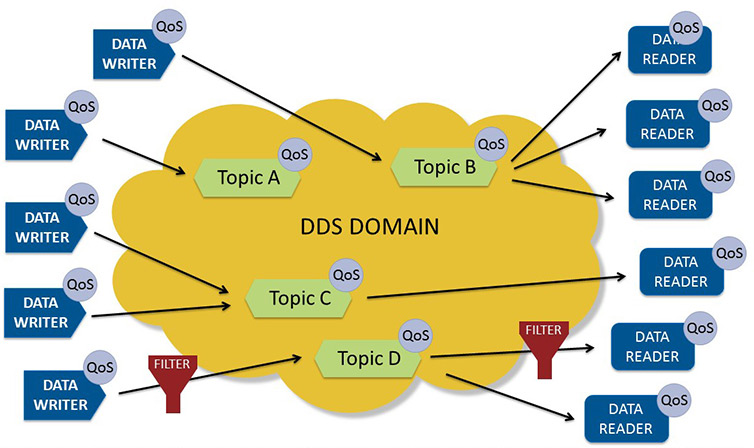
\includegraphics[width=0.8\textwidth]{Images/chap3/dds.jpg}
    \vspace{0.5cm}
    \caption{DDS enables QoS-controlled data-sharing via a publish/subscribe model on named Topics, featuring time/content filtering and strict isolation between independent domains.}
    \label{fig:dds}
\end{figure}

Unlike traditional Remote Procedure Call (RPC) frameworks or conventional Message-Oriented Middleware (MOM), DDS focuses intrinsically and exclusively on the data itself. The middleware is inherently aware of the data schema, strictly defined using the OMG Interface Definition Language (IDL) or the Extensible and Dynamic Topic Types for DDS (DDS-XTypes) specification. This profound data awareness allows the middleware stack to autonomously perform complex content-based filtering, data lifecycle management, and state propagation without requiring application-level intervention. 

The definition of DDS extends beyond mere data transfer; it encapsulates a holistic ecosystem for real-time state management. By standardizing serialization, discovery, security, and delivery guarantees, DDS allows automotive software engineers to concentrate exclusively on application-level logic rather than network-level fault tolerance, fundamentally accelerating the development cycle.



\subsubsection{Public-Subscribe Communication Model}

The architectural foundation of the Data Distribution Service is the Data-Centric Publish-Subscribe (DCPS) model. The DCPS model distinguishes itself by prioritizing the management of stateful data over the mere routing of transient, stateless events. Information is strictly typed and categorized into distinct Topics, and the fundamental unit of information sharing is the structured data-object within these Topics.

The overarching boundary within the DCPS model is the \texttt{Domain}, representing a logically isolated communication space. Applications operating within different domains cannot communicate with one another. An application enters a domain by instantiating a \texttt{DomainParticipant}, which serves as the primary factory and container for all subsequent DDS entities, managing the discovery of other participants within the domain.

Data production is managed by \texttt{Publisher} entities, which act as organizational factories for \texttt{DataWriter} objects. A \texttt{DataWriter} is strongly typed to a specific Topic and is the sole authorized mechanism through which an application can introduce new data samples into the Global Data Space. Conversely, data consumption is handled by \texttt{Subscriber} entities, which function as factories for \texttt{DataReader} objects. A \texttt{DataReader} securely binds to a specific Topic and provides the receiving application with access to the incoming data samples through asynchronous callbacks or synchronous polling.

A defining characteristic of the DCPS model is its robust type system and the critical distinction between ``Instances'' and ``Samples.'' When a Topic data type is defined, specific fields can be explicitly annotated with a \texttt{@key} identifier. The unique mathematical combination of these key values identifies a specific ``Instance'' of the Topic. Every time a \texttt{DataWriter} publishes data for a specific key combination, it generates a new ``Sample'' of that Instance, representing an update to its state. This deeply data-centric approach ensures that subscribers are not merely receiving disconnected packets, but are instead maintaining a synchronized, localized object model that accurately reflects the distributed state of the environment.

\subsubsection{Quality of Service (QoS) Policies}

The defining technical superiority of DDS lies in its extensive Quality of Service (QoS) framework. DDS provides distinct, configurable QoS policies that strictly dictate the behavior of the middleware, decisively separating the functional requirement for data transfer from the implementation of network retries, pacing, and acknowledgments.

Each entity within the DCPS model possesses an associated QoS configuration. A fundamental principle governing DDS QoS is the Request/Offer semantic. A \texttt{DataReader} explicitly requests a certain level of service, and a \texttt{DataWriter} explicitly offers a specific level of service. For a communication channel to be successfully established (matching), the offered QoS must meet or exceed the requested QoS. If incompatible, the middleware prevents association and alerts the application.

The most critical QoS policies utilized within real-time automotive systems include:

\begin{table}[h!]
\centering
\renewcommand{\arraystretch}{1.3}
\begin{tabular}{|p{0.18\textwidth}|p{0.2\textwidth}|p{0.55\textwidth}|}
\hline
\textbf{QoS Policy} & \textbf{Target Entity} & \textbf{Description and Automotive Application} \\
\hline
\textbf{Reliability} & Writer, Reader, Topic & Defines if delivery is guaranteed. \texttt{BEST\_EFFORT} (no retransmissions) suits high-frequency sensor streams. \texttt{RELIABLE} enforces TCP-like reliability over UDP, mandated for safety-critical state transitions. \\
\hline
\textbf{Durability} & Writer, Reader, Topic & Controls data availability to late-joining subscribers. \texttt{VOLATILE} only serves active readers. \texttt{TRANSIENT\_LOCAL} automatically forwards stored past samples to new readers, critical for initialization states. \\
\hline
\textbf{History} & Writer, Reader, Topic & Dictates local cache management. \texttt{KEEP\_LAST} stores only the most recent $N$ samples. \texttt{KEEP\_ALL} retains every sample until successfully delivered to all reliable readers. \\
\hline
\textbf{ResourceLimits} & Writer, Reader, Topic & Governs maximum physical memory allocation (queue bounds). Crucial for embedded ECUs to prevent out-of-memory exceptions during runtime. \\
\hline
\textbf{DestinationOrder} & Writer, Reader, Topic & Determines logical message order during simultaneous writes. Ordering by \texttt{SOURCE\_TIMESTAMP} ensures deterministic behavior in multi-sensor fusion algorithms. \\
\hline
\textbf{Lifespan} & Writer, Reader, Topic & Sets the relevance duration of a sample. Expired data is automatically purged, mathematically guaranteeing that ADAS modules do not react to stale perceptions. \\
\hline
\textbf{UserData} & Participant, Reader, Writer & Attaches custom byte sequences. AUTOSAR specifically utilizes this during discovery to encode Service IDs and contract versions in participant announcements. \\
\hline
\textbf{Liveliness} & Writer, Reader, Topic & Asserts the time interval a node must demonstrate activity. If a sensor node fails to assert liveliness, subscribers are alerted to transition to a safe state. \\
\hline
\end{tabular}
\end{table}

\subsubsection{DDS Real-Time Publish Subscribe (RTPS) Protocol}

While the DDS specification defines the APIs and QoS semantics, the physical interoperability of disparate DDS implementations is governed by the Real-Time Publish Subscribe (RTPS) protocol. Standardized as the DDSI-RTPS, this specification guarantees that a lightweight sensor node can seamlessly communicate with an HPC node running an enterprise DDS implementation, irrespective of the underlying vendor.

RTPS leverages the connectionless, best-effort, and multicast capabilities of UDP/IP to achieve massive scalability, while independently layering a sophisticated reliability protocol on top of it. The RTPS architecture is structurally divided into two primary operational modules: the Discovery Module and the Behavior Module.

The Discovery Module is responsible for the dynamic ``plug-and-play'' nature of DDS. It operates in two sequential phases: the Simple Participant Discovery Protocol (SPDP) and the Simple Endpoint Discovery Protocol (SEDP). During SPDP, \texttt{DomainParticipants} periodically multicast compact announcement messages containing their GUIDs, locators, and basic QoS settings. Upon receiving an unknown announcement, participants initiate the SEDP phase to directly exchange detailed information regarding their internal \texttt{DataWriters} and \texttt{DataReaders}. This completely decentralized architecture fundamentally eliminates single points of failure.

The Behavior Module defines the strictly regulated message exchanges. To fulfill \texttt{RELIABLE} QoS obligations over UDP, RTPS utilizes a Heartbeat and Negative Acknowledgment (NACK) paradigm. A \texttt{DataWriter} periodically multicasts Heartbeats detailing available sequences. If a \texttt{DataReader} identifies missing sequences, it responds with an ACKNACK, prompting the \texttt{DataWriter} to retransmit only the requested samples. Furthermore, DDSI-RTPS specifies the binary layout of messages, allowing microcontrollers with different native byte architectures to parse the data seamlessly.

\subsubsection{DDS in Adaptive AUTOSAR}

The incorporation of DDS into the AUTOSAR Adaptive Platform provides a highly scalable alternative to SOME/IP. Within the AUTOSAR specification, the Communication Management (\texttt{ara::com}) cluster translates language-agnostic \texttt{ServiceInterface} models into concrete DDS entities, Topics, and RTPS wire payloads.

\textbf{Service Discovery Mechanisms}

The DDS Network Binding provides two methodologies for Service Discovery:

\begin{enumerate}
\item \textbf{Service Discovery via Domain Participant USER\_DATA QoS policy:} This approach natively leverages the built-in RTPS Participant Discovery phase (SPDP). The middleware injects a precisely formatted string into the \texttt{USER\_DATA} QoS policy of its \texttt{DomainParticipant} containing the Service ID, Instance ID, and version. Client proxies parse this string to verify compatibility. Because this utilizes intrinsic DDS discovery traffic without creating additional entities, it is exceptionally resource-efficient.
\item \textbf{Service Discovery via Topic:} For highly complex topologies, the offering service explicitly publishes a dedicated \texttt{ServiceAnnouncementMessage} over a standardized \texttt{ara.com://services/discovery} topic, utilizing the Service ID and Instance ID as cryptographic keys.
\end{enumerate}

\textbf{Mapping of Events and Triggers}

An \texttt{Event} maps fundamentally to a single, dedicated DDS Topic. The payload is serialized into an IDL struct that inevitably includes an \texttt{@key uint16 instance\_id} field alongside the data. This key ensures logical segregation by the middleware's management queues. \texttt{Triggers} map similarly but are entirely devoid of a functional data payload; they utilize merely the key to serve as an asynchronous signaling mechanism.

\textbf{Mapping of Fields}

A \texttt{Field} is systematically decomposed for network transmission. If it possesses a notification property, a dedicated DDS Topic pushes state updates like an Event. If it has getter or setter attributes, a Request/Reply Topic pair is generated identically to the Method mapping, enabling RPC over DDS state management.

\textbf{Data Serialization and Security Integration}

The DDS binding relies on the OMG DDS-XTypes specification for data serialization, seamlessly handling complex C++ structures while managing byte-endianness transparently. 

For security, the binding natively supports the OMG DDS-Security standard via a plugin architecture, providing Authentication, Access Control, and Cryptography at the individual submessage level. AUTOSAR mandates that Adaptive Applications must enforce Identity and Access Management (IAM) grants through deployed DDS Security policies, allowing for highly granular configurations that minimize cryptographic overhead while maximizing real-time throughput.




\subsection{AUTOSAR Runtime for Adaptive applications (\texttt{ara})}

\begin{figure}[h]
    \centering
    \includegraphics[width=0.9\textwidth]{Images/chapter2/AP_Arch.png}
    \vspace{0.5cm}
    \caption{Logical View of AUTOSAR Adaptive Platform Architecture \cite{autosar_sw_arch}}
    \label{fig:autosar_adaptive_arch_logic}
\end{figure}


The AUTOSAR Runtime for Adaptive applications (\texttt{ara}) acts as the standardized runtime environment for Adaptive Applications (AA). It abstracts the underlying system features and provides a uniform interface for applications to interact with the platform. As illustrated in Figure \ref{fig:autosar_adaptive_arch_logic}, the architecture is composed of the following key blocks:

\paragraph*{Adaptive Applications (AA):} These are user applications running on top of the Adaptive Platform. They implement specific automotive functions (e.g., automated driving logic, infotainment) and interact with the platform exclusively through the \texttt{ara} interfaces. This design decouples the application logic from the underlying OS and hardware, ensuring portability.

\paragraph*{ARA Interface:} \texttt{ara} consists of a set of Application Programming Interfaces (APIs), primarily standardized in C++. These interfaces allow AAs to access functionalities provided by the Functional Clusters. From the application's perspective, the interface is uniform regardless of whether the underlying functionality belongs to the Foundation or Services layer.


\paragraph*{Functional Clusters (FC):} Functional Clusters are logical groupings of platform functionality. They are responsible for providing specific services to the applications. They are categorized into two types:

\textbf{Adaptive Platform Foundation:} This layer provides the fundamental functionalities required to run the system and applications. It includes core services such as Execution Management (\texttt{ara::exec}), Communication Management (\texttt{ara::com}), Logging (\texttt{ara::log}), Persistency (\texttt{ara::per}), etc. These clusters behave similarly to operating system services.
    
\textbf{Adaptive Platform Services:} This layer provides platform-standard services that are more domain-specific but still standardized, such as Update and Configuration Management (\texttt{ara::ucm}), State Management (\texttt{ara::sm}), and Network Management (\texttt{ara::nm}).

Under the hood, the implementation of these interfaces may involve library calls within the application's process space or Inter-Process Communication (IPC) with daemon processes, but this complexity is hidden from the application developer.



In the context of this project, our primary focus lies within the Application Layer (Adaptive Applications). Consequently, our discussion will center on the essential Functional Clusters that support application runtime and interaction: Execution Management (\texttt{ara::exec}), Communication Management (\texttt{ara::com}), and Log and Trace (\texttt{ara::log}). Additionally, to address the specific requirements of our machine learning use case, we will integrate non-platform services, specifically utilizing the OpenCV library (namespace \texttt{cv}) for advanced image pre-processing and computer vision tasks. 



\subsection{Execution Management (\texttt{ara::exec})} 

Execution Management is responsible for all aspects of the system execution, including the initialization of the Adaptive Platform and the lifecycle management of Processes. Acting as the entry point of the AUTOSAR Adaptive Platform, Execution Management is started by the Operating System during system boot and subsequently launches the Functional Clusters and Adaptive Applications based on the configuration defined in the Machine Manifest and Execution Manifests.

It controls the startup and shutdown of these Processes according to defined Function Group States, ensuring that the specific set of processes required for a given state are active. While the Operating System performs the actual runtime scheduling, Execution Management configures the OS to enforce scheduling parameters and resource limits. This includes assigning processes to Resource Groups to limit CPU time and memory usage, thereby supporting freedom from interference between applications. Furthermore, Execution Management enables deterministic execution through the \texttt{DeterministicClient} API, allowing for the control of process-internal cycles and data determinism.

To establish a Trusted Platform, Execution Management maintains a chain of trust originating from a Trust Anchor. During authenticated startup, it validates the authenticity and integrity of Adaptive Applications and prevents the execution of any process if security violations are detected.

\subsubsection{Block View Diagram } 

\textbf{Interface for state reporting: }
All processes started by Execution Management (i.e. all processes of the AUTOSAR Adaptive Platform and all processes of Adaptive Applications) shall report their execution state back to Execution Management via the ExecutionClient interface

\begin{figure}[h]
    \centering
    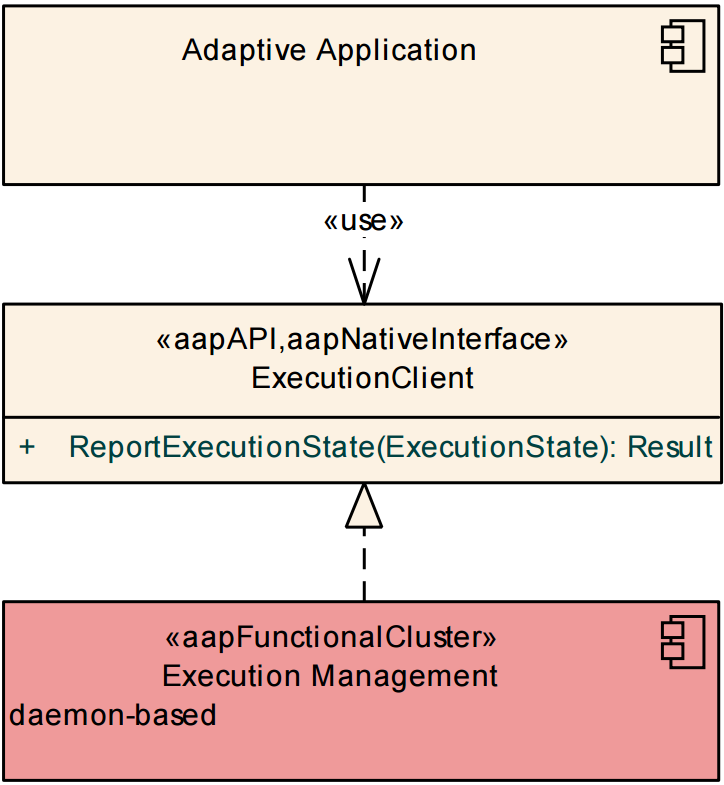
\includegraphics[width=0.5\textwidth]{Images/chapter2/em_interface.png}
    \vspace{0.5cm}
    \caption{Interface for state reporting \cite{autosar_sw_arch}}
    \label{fig:em_interface}
\end{figure}

\textbf{Provided Interfaces:} \texttt{ara::exec::ExecutionClient} will provide the interface reporting the execution state of the process to Execution Management. \texttt{ara::exec::StateClient} will Requests Function Group State transitions and retrieves execution errors.

\begin{figure}[h]
    \centering
    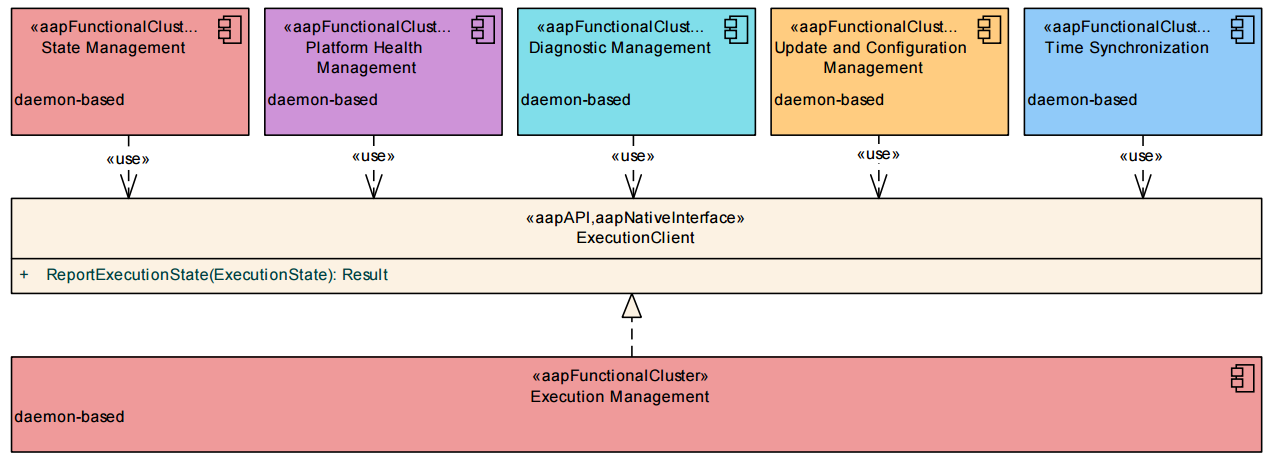
\includegraphics[width=0.9\textwidth]{Images/chapter2/em_provided_execcli.png}
    \vspace{0.5cm}
    \caption{Users of ExecutionClient Interface \cite{autosar_sw_arch}}
    \label{fig:em_provided_execcli}
\end{figure}

\begin{figure}[h]
    \centering
    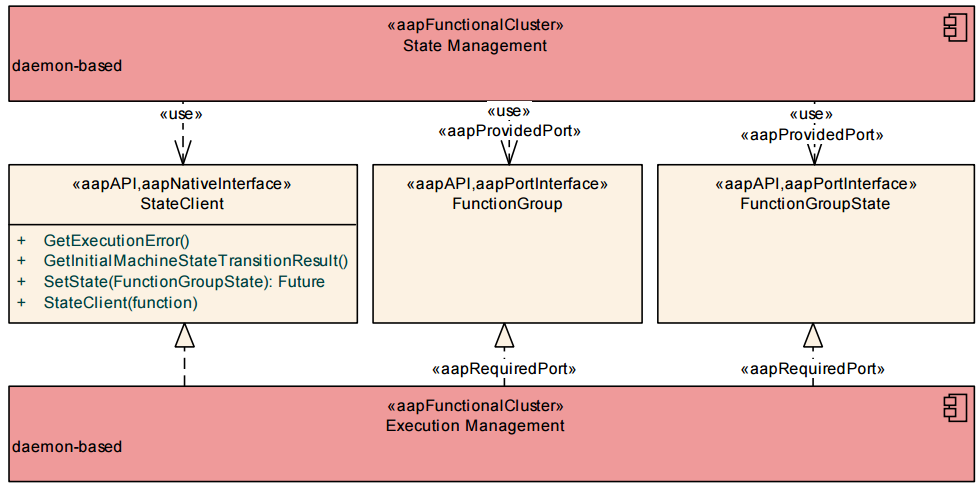
\includegraphics[width=0.9\textwidth]{Images/chapter2/em_provided_sm.png}
    \vspace{0.5cm}
    \caption{Users of State Management Interface \cite{autosar_sw_arch}}
    \label{fig:em_provided_sm}
\end{figure}

\newpage
\textbf{Required Interfaces:} \begin{itemize} 
    \item \texttt{Log and Trace::Logger}: Execution Management shall use this interface to log standardized messages. 
    \item \texttt{Persistency::KeyValueStorage}: Execution Management should use this interface to read and write persistent data. 
    \item \texttt{Platform Health Management::SupervisedEntity}: Execution Management shall use this interface to enable supervision of its process(es) by Platform Health Management. 
    \item \texttt{Time Synchronization::SynchronizedTimeBaseConsumer}: The \texttt{DeterministicClient} implementation in Execution Management should use this interface to synchronize execution. 
    \item \texttt{Manifest Accessor}: Execution Management shall use this interface to read the configuration of its \texttt{DeterministicClient} and information about Function Groups and Processes from the Manifests. 
    \item \texttt{Operating System::Multi-Process System Interface}: Execution Management shall use this interface to start, configure, and control OS-level processes. 
\end{itemize}

\begin{figure}[h]
    \centering
    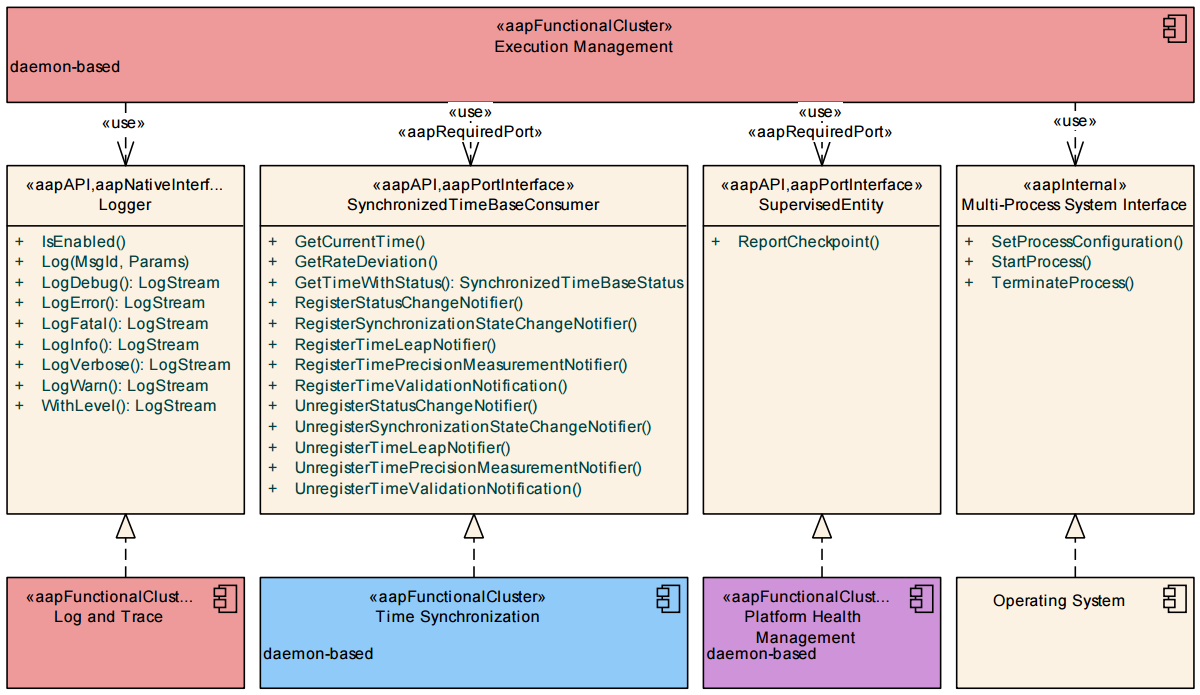
\includegraphics[width=0.9\textwidth]{Images/chapter2/em_required.png}
    \vspace{0.5cm}
    \caption{Required Interfaces of Execution Management \cite{autosar_sw_arch}}
    \label{fig:em_required}
\end{figure}


\newpage
\subsubsection{System Startup} 

\begin{figure}[h]
    \centering
    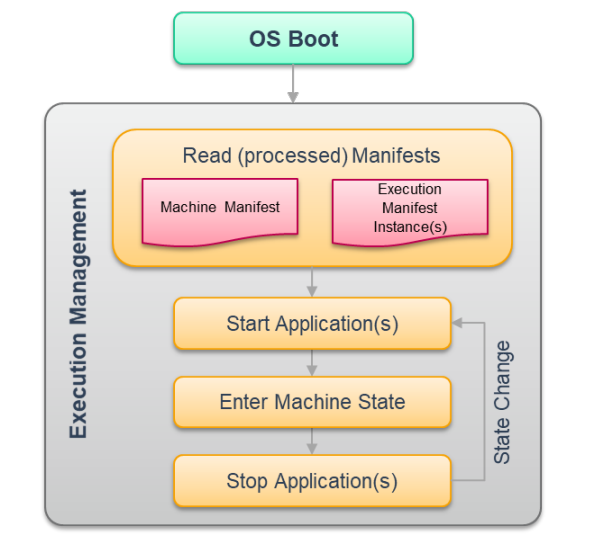
\includegraphics[width=0.5\textwidth]{Images/chapter2/EM_APStartup.png}
    \vspace{0.5cm}
    \caption{AP Startup Sequence \cite{autosar_exec_mgmt}}
    \label{fig:em_ap_startup}
\end{figure}

\textbf{Startup Sequence:} When the Machine is powered on, the Operating System (OS) is initialized first. Immediately following OS initialization, Execution Management is launched as the Platform's initial process. It is then the responsibility of Execution Management to launch the other platform-level processes that constitute the Functional Clusters of the Adaptive Platform Foundation. Once the Adaptive Platform Foundation is fully operational, Execution Management proceeds to launch the processes associated with Adaptive Applications. The specific startup order for both platform-level and application-level processes is determined by Execution Management, utilizing the configuration defined in the Machine Manifest and the dependencies specified in the Execution Manifest.

\textbf{Application Structure:} An Adaptive Application is composed of multiple Executable elements, which generally correspond to executable files located on the filesystem. To allow for flexible behavior, each Executable can define multiple Process configurations (and therefore distinct startup configurations). The active configuration is determined by the specific Function Group States in which the Executable is currently active.

\textbf{Trusted Platform:} To ensure system security, Execution Management optionally supports an authenticated startup process. This mechanism establishes a Trusted Platform by maintaining a chain of trust originating from a Trust Anchor. During this phase, Execution Management validates the authenticity and integrity of applications before they are launched. If any violations are detected during validation, Execution Management will prevent the execution of the compromised application.

\textbf{Manifests:}

\begin{figure}[h]
    \centering
    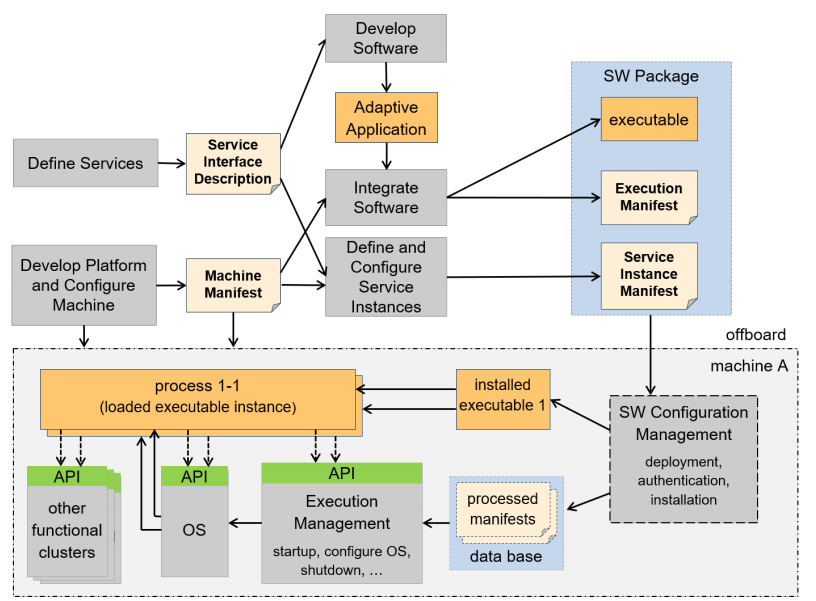
\includegraphics[width=0.9\textwidth]{Images/chapter2/ap_dev_flow.png}
    \vspace{0.5cm}
    \caption{Application Development Flow \cite{autosar_exec_mgmt}}
    \label{fig:ap_dev_flow}
\end{figure}

Manifests serve as the standardized format for description and configuration within the AUTOSAR Adaptive Platform, effectively bridging the gap between system design and runtime execution. To address the distinct phases of the development lifecycle, Manifests are categorized into four specific types. {Application Design} specifies the architectural aspects of the software; while not deployed itself, it aids in defining deployment configurations. The {Execution Manifest} details deployment parameters—such as startup dependencies and resource usage—and is bundled directly with the application executable. Similarly, the {Service Instance Manifest} accompanies the executable code to configure service-oriented communication bindings and transport protocols. Finally, the {Machine Manifest} describes the configuration of the underlying computing machine and the Adaptive Platform foundation, independent of the specific applications hosted on the system. As in Figure \ref{fig:ap_dev_flow}, the application development flow will show how manifests are created. 

\subsubsection{\texttt{ara::exec} Responsibility}

% Execution Management functions as a critical functional cluster within the Adaptive Platform Foundation, serving as the primary entity responsible for managing all aspects of system execution, which encompasses the initialization of the platform as well as the startup and shutdown of Applications. It operates in close conjunction with the Operating System, specifically configuring it to handle the run-time scheduling of Applications. The core unit managed by this cluster is the Modelled Process, which is an instance of an Executable. Execution Management is responsible for the lifecycle of these processes, performing tasks such as creation and termination based on specific information contained within Manifest files, specifically the Execution Manifest and the Machine Manifest.

% A central responsibility of Execution Management is to determine the precise timing and sequence for starting or stopping processes based on the configuration data extracted from the manifests. It derives the launching order of Applications to ensure the proper startup of the AUTOSAR Adaptive Platform, ensuring that processes are started in a sequence that respects declared Execution Dependencies. This dependency management ensures that applications are active only when the services they require are available and are terminated only after their services are no longer required. To maintain strict control over the system, Execution Management is designed to be the sole entity responsible for starting processes and must restrict the rights of the processes it launches so they cannot start other processes themselves.

% In addition to lifecycle management, Execution Management is integral to the platform's State Management. It supports the execution of specific Modelled Processes depending on the current Function Group State or Machine State. Execution Management initiates state transitions, such as the transition from the Off state to the Startup state during the platform's boot phase. During these transitions, it is responsible for terminating processes that are no longer needed in the requested state and starting those that are required, all while monitoring process termination and startup timeouts to ensure the transition completes successfully or handles errors appropriately. While Execution Management facilitates these changes, it hands over the responsibility for requesting subsequent state changes to the State Management cluster after the initial startup transition is confirmed.

% The responsibility of Execution Management extends to the configuration of the Operating System to enable appropriate resource management and scheduling. Although the Operating System performs the actual run-time scheduling, Execution Management is responsible for initializing the OS with the necessary configuration parameters derived from the manifests. This includes the configuration of scheduling policies and priorities for the initial threads of processes, as well as the assignment of processes to specific processor cores. Furthermore, Execution Management supports resource limitation by configuring budgets for CPU usage and memory consumption for groups of processes, ensuring that applications operate within defined constraints to maintain system stability.

% Finally, Execution Management plays a pivotal role in ensuring the security and determinism of the platform. It is responsible for supporting a Trusted Platform by ensuring that the integrity and authenticity of all Executables and their associated data, such as manifests, are verified before any process is started. In the event of a failed check, it executes defined measures to prevent compromised software from running. Additionally, Execution Management provides support for Deterministic Execution, allowing for calculations that are time and data deterministic. This involves providing APIs and mechanisms that support the control of process-internal cycles and deterministic worker pools, which are essential for safety-critical systems requiring reproducible behavior.

Execution Management (\texttt{ara::exec}) is a core functional cluster in the Adaptive AUTOSAR platform. It acts as the main unit for managing system execution, including platform initialization and the lifecycle of applications. Working closely with the Operating System (OS), it creates and terminates processes based on the rules defined in the Execution and Machine Manifest files. A key responsibility is controlling the exact launching order of applications to respect their dependencies. To keep strict control over the system, Execution Management is the only component allowed to start processes, ensuring that applications are active only when their required services are ready.

In addition to lifecycle control, Execution Management plays an important role in State Management and OS configuration. It starts or stops specific processes depending on the current machine or function group state. For example, during the boot phase, it handles the transition from the ``Off'' state to ``Startup,'' ensuring that old processes are terminated and new ones are launched properly. Furthermore, Execution Management configures the OS to manage resources efficiently. Although the OS handles the actual run-time scheduling, Execution Management sets up the initial scheduling policies, assigns processes to specific processor cores, and limits CPU and memory usage to keep the system stable.

Finally, Execution Management ensures the security and reliability of the platform. It supports a Trusted Platform by verifying the integrity and authenticity of all executables and manifests before any process begins. If a check fails, it takes action to stop compromised software from running. Additionally, it supports Deterministic Execution, which is crucial for safety-critical systems. By providing specific mechanisms and APIs, Execution Management guarantees that calculations remain consistent in terms of both time and data, ensuring reproducible and safe behavior across the system.


% \subsubsection{Process Lifecycle Management}

% In the AUTOSAR Adaptive Platform, the lifecycle of a process is viewed from two distinct perspectives: the {Process State}, which is the external view maintained by Execution Management for orchestration, and the {Execution State}, which represents the internal lifecycle from the perspective of the application process itself.

% \begin{figure}[h]
%     \centering
%     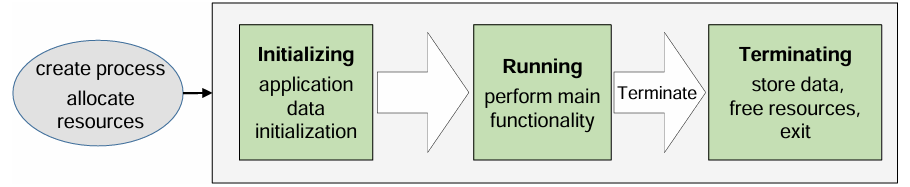
\includegraphics[width=0.8\textwidth]{Images/chapter2/em_execstate.png}
%     \vspace{0.5cm}
%     \caption{EM Execution State \cite{autosar_exec_mgmt}}
%     \label{fig:em_execstate}
% \end{figure}

% Because the process and Execution Management run as independent operating system processes, they execute asynchronously. The Execution State serves as the synchronization mechanism between the application's internal progress and the Execution Management's control logic. This separation allows the internal state of a process to evolve without strictly coupling it to the internal state machine of Execution Management.

% \paragraph*{The Execution State Lifecycle}
% While the API explicitly defines the \texttt{kRunning} state, the full lifecycle includes implied states that dictate how a process initializes, runs, and shuts down.

% \textbf{Initializing (Implied State):}
% The "Initializing" state is an implied state that is not explicitly defined in the \texttt{ExecutionState} enumeration but is recognized operationally by Execution Management. This phase, {Start}, begins immediately when the OS process is created and code execution commences. During the {Activity} phase, the process performs necessary setup tasks, such as memory allocation, variable initialization, and checking configuration files. The state concludes, marked as {End}, when the process explicitly notifies Execution Management that it is ready to operate.

% \textbf{Running (\texttt{kRunning}):}
% The \texttt{kRunning} state is the primary active state defined in the API (\texttt{ara::exec::ExecutionState::kRunning}). A process must explicitly report this state, a {Transition}, to Execution Management once initialization is complete. Regarding {Timing Requirement}, processes are expected to report \texttt{kRunning} after internal initialization but generally before completing Service Discovery. If a process waits until Service Discovery is finished to report \texttt{kRunning}, it may cause non-deterministic delays for other processes that have execution dependencies on it. Once \texttt{kRunning} is reached, the process is considered in its {Operational Context}, ready to perform its main functionality.

% \textbf{Terminating (Implied State):}
% Like initialization, "Terminating" is a state characterized by the reaction to a termination request rather than a specific API call from the process. The {Trigger} for this phase is Execution Management sending a \texttt{SIGTERM} signal to the process. Upon receiving \texttt{SIGTERM}, the {Activity} involves the process saving persistent data, closing file handles, and freeing resources. The {Completion} of this state occurs when the process exits with the status \texttt{EXIT\_SUCCESS} (0).

% \paragraph*{API and Reporting Mechanism}
% To synchronize with Execution Management, processes utilize the \texttt{ara::exec::ExecutionClient} class. The {Reporting API} allows the process to report its state using the method \texttt{ReportExecutionState}, for example, \texttt{ReportExecutionState(kRunning)}. The {Scope of Authority} restricts a process to reporting only its own Execution State. Execution Management performs {Validation} on state transitions; if a process attempts to report \texttt{kRunning} when Execution Management believes the process is already in a state other than "Starting" (e.g., if it is already running), the API will return the error \texttt{kInvalidTransition}.

% \paragraph*{Process Categorization: Reporting vs. Non-Reporting}
% Execution Management supports two distinct behaviors regarding Execution State reporting, configured via the Execution Manifest.

% \textbf{Reporting Processes:}
% This is the standard behavior for AUTOSAR Adaptive Applications. These processes exhibit a specific \textbf{Behavior} where they are aware of the \texttt{ara::exec} API and explicitly call \texttt{ReportExecutionState(kRunning)}. For {Synchronization}, Execution Management waits for this specific report before considering the process to be in the "Running" Process State.

% \textbf{Non-Reporting Processes:}
% This category supports legacy applications or prototypes that were not designed with the AUTOSAR Adaptive Platform in mind and do not contain AUTOSAR-specific API calls. Their {Behavior} is characterized by not calling \texttt{ReportExecutionState}. Instead, an {Implicit Transition} occurs where Execution Management treats these processes as "Running" immediately after the OS process is created and resources are allocated. {Restrictions} apply: if a configured Non-reporting Process attempts to use the API to report its state, Execution Management considers this a violation and returns a \texttt{kCommunicationError}. Due to {Limitations}, because they effectively skip the "Initializing" phase from EM's perspective, "Running" execution dependencies are satisfied immediately upon process creation, which may require the use of a "Companion Process" to bridge dependency gaps.

% \paragraph*{Termination and Error Handling:}
% Proper lifecycle management requires strict adherence to termination protocols. {Graceful Termination} requires a process to exit with status 0 (\texttt{EXIT\_SUCCESS}) to indicate a successful shutdown. In contrast, an {Unexpected Termination} occurs if a process exits with a non-zero status, or if it terminates before reporting \texttt{kRunning}, which Execution Management classifies as such. The {Consequences} of an unexpected termination trigger error handling within the State Management functional cluster, setting the affected Function Group to an "Undefined Function Group State" and reporting an \texttt{ExecutionError}.



% The {Process State} is the internal state machine maintained by Execution Management to track the lifecycle of a Modelled Process. While the Execution State reflects the application's internal progress, the Process State reflects Execution Management's orchestration view. Execution Management maintains this state independently to manage timeouts, handle errors, and resolve Execution Dependencies without being strictly coupled to the internal logic of the application process.

% \begin{figure}[h]
%     \centering
%     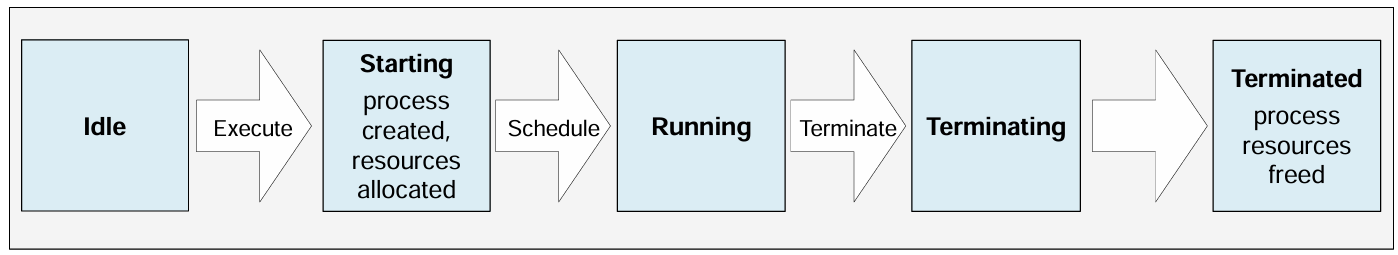
\includegraphics[width=0.9\textwidth]{Images/chapter2/em_processstate.png}
%     \vspace{0.5cm}
%     \caption{Process State \cite{autosar_exec_mgmt}}
%     \label{fig:em_processstate}
% \end{figure}

% \paragraph*{The Process State Lifecycle}
% The lifecycle of a process, as managed by Execution Management, consists of five distinct states. Transitions between these states are driven by API calls, OS signals, and internal configuration logic.

% \textbf{Idle:} The Idle state represents the dormancy of a process. This state applies prior to the creation of the Operating System (OS) process and prior to the allocation of any OS resources. In this state, the process exists only as a configuration entry in the Execution Manifest. It consumes no CPU time or memory. The process leaves the Idle state when Execution Management initiates the startup sequence required by a Function Group State change.

% \textbf{Starting:} The Starting state covers the physical launch and initialization phase of the process. Execution Management transitions a process to ``Starting" immediately upon creating the OS process and allocating the necessary resources. During this phase, Execution Management monitors the ``Startup Timeout." This is the time allowed between the request for process creation and the process successfully reporting \texttt{kRunning}. To ensure state consistency, if a Reporting Process attempts to report \texttt{kRunning} but Execution Management does not consider it to be in the "Starting" state (e.g., if it is already Running), the API call is rejected with the error \texttt{kInvalidTransition}.

% \textbf{Running:} The Running state indicates that the process is fully active and functional. The criteria for entering this state vary by process configuration:
% The process transitions to "Running" only after it explicitly reports the \texttt{kRunning} Execution State via the API. This serves as a synchronization barrier, ensuring dependent processes do not start until this process is truly ready. Because these processes do not use the AUTOSAR API, Execution Management implicitly transitions them to "Running" immediately after resource allocation and process creation. If a process fails to reach the "Running" state within the configured timeout, Execution Management may attempt to restart it a configured number of times (\texttt{numberOfRestartAttempts}) before declaring a failure and stopping the Function Group State transition.

% \textbf{Terminating:} The Terminating state represents the shutdown phase where the process is expected to release resources and save data. This state applies from the moment Execution Management sends the \texttt{SIGTERM} signal to the process. Execution Management monitors the time the process spends in this state. If the process does not exit within the configured termination timeout, Execution Management considers the process unresponsive and requests the Operating System to forcibly terminate it (typically via \texttt{SIGKILL}). Even if a timeout occurs and forced termination is required, Execution Management continues the state transition to ensure the target Function Group State is eventually reached.

% \textbf{Terminated:} The Terminated state marks the successful conclusion of a process execution instance. This state applies after the process has successfully exited and all process resources have been freed by the Operating System. Execution Management detects this state by observing the exit status of the OS process (e.g., utilizing \texttt{waitpid} on POSIX systems). A normal termination requires an exit status of \texttt{EXIT\_SUCCESS} (0). Any other exit code, or termination by an unhandled signal, is classified as an "Unexpected Termination".


% Although both Idle and Terminated implies that no code is executing and no resources are allocated, Execution Management treats them as semantically distinct for dependency resolution. In {Idle} state, the process has not run in the current lifecycle context. In {Terminated} state, the process has run, finished its task, and shut down gracefully. This distinction allows for Self-Terminating Processes. A dependent process can be configured to start only after a provider process has reached the "Terminated" state (e.g., "Start Data Analyzer" only after "Data Collector" is "Terminated"). This dependency cannot be satisfied if the provider is merely "Idle".

% \paragraph*{Error Handling and Unexpected States:}
% Execution Management actively monitors processes for deviations from the expected lifecycle. {Unexpected Termination:} If a process terminates without a request (or exits with a non-zero status) while in the Running state or during startup, Execution Management flags this as an Unexpected Termination. {Consequences:} The event is logged. The Function Group to which the process belongs is set to an Undefined Function Group State. An \texttt{ExecutionError} is reported via the State Client API to allow State Management to decide on recovery actions (e.g., restarting the Machine or switching to a safe state).

% \paragraph*{Role in Execution Dependencies:}
% Process States are the fundamental building blocks for defining startup and shutdown sequencing in the Execution Manifest. Dependencies are defined as \texttt{<Process>.<State>} pairs. 
% \begin{itemize}
%     \item \textbf{Running Dependency:} Ensures a service provider is fully operational before a dependent consumer starts. The dependent waits for the provider to reach the Running Process State. 
%     \item \textbf{Terminated Dependency:} Used primarily for sequential tasks. The dependent waits for the provider to reach the Terminated Process State. 
%     \item \textbf{Scope Constraint:} Execution Management only resolves dependencies within a single Function Group State. It considers it an error if a process depends on another process that is not part of the same Function Group State.
% \end{itemize}

\subsubsection{Process Lifecycle Management}

In the AUTOSAR Adaptive Platform, process lifecycle management operates on two distinct but synchronized levels: the {Execution State} (the application's internal perspective) and the {Process State} (the orchestration perspective maintained by Execution Management). Because the application and Execution Management run asynchronously as independent OS processes, these dual states decouple internal initialization logic from the broader system state machine.

\paragraph*{The Execution State (Application Perspective)}
The Execution State in the Figure~\ref{fig:em_execstate} represents the application's internal lifecycle. Upon OS process creation, an application implicitly enters an "Initializing" phase to allocate resources and perform setup tasks. Once initialization is complete (but crucially, before finalizing Service Discovery to avoid dependency deadlocks), a standard AUTOSAR process must explicitly notify Execution Management by calling \texttt{ara::exec::ExecutionClient::ReportExecutionState(kRunning)}. When the application needs to shut down---typically triggered by a \texttt{SIGTERM} signal from Execution Management---it implicitly enters the "Terminating" phase, releases resources, and concludes by exiting with \texttt{EXIT\_SUCCESS} (0) to signal a graceful termination.

\begin{figure}[h]
    \centering
    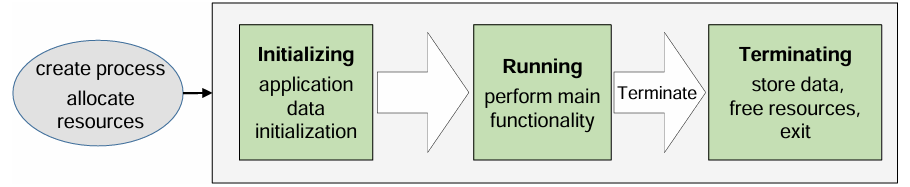
\includegraphics[width=0.8\textwidth]{Images/chapter2/em_execstate.png}
    \vspace{0.5cm}
    \caption{EM Execution State \cite{autosar_exec_mgmt}}
    \label{fig:em_execstate}
\end{figure}

\paragraph*{The Process State (Orchestration Perspective)}
Conversely, the Process State is maintained internally by Execution Management to resolve execution dependencies, manage timeouts, and enforce error handling. The lifecycle encompasses five states, which is presented in Figure~\ref{fig:em_processstate}:
\begin{itemize}
    \item \textbf{Idle:} The process exists only as a configuration entry; no OS resources are allocated.
    \item \textbf{Starting:} The OS process is created, and Execution Management monitors a "Startup Timeout" while waiting for the application to report readiness.
    \item \textbf{Running:} The process has successfully reported \texttt{kRunning}. Dependent applications configured with a "Running Dependency" on this process are now permitted to start. (Note: Non-AUTOSAR legacy applications are implicitly transitioned to this state immediately after OS creation).
    \item \textbf{Terminating:} Execution Management has issued a \texttt{SIGTERM} and monitors a termination timeout. If the process hangs, it is forcibly terminated via \texttt{SIGKILL}.
    \item \textbf{Terminated:} The OS process has successfully exited. This distinct state enables "Terminated Dependencies" for sequential task execution.
\end{itemize}

\begin{figure}[h]
    \centering
    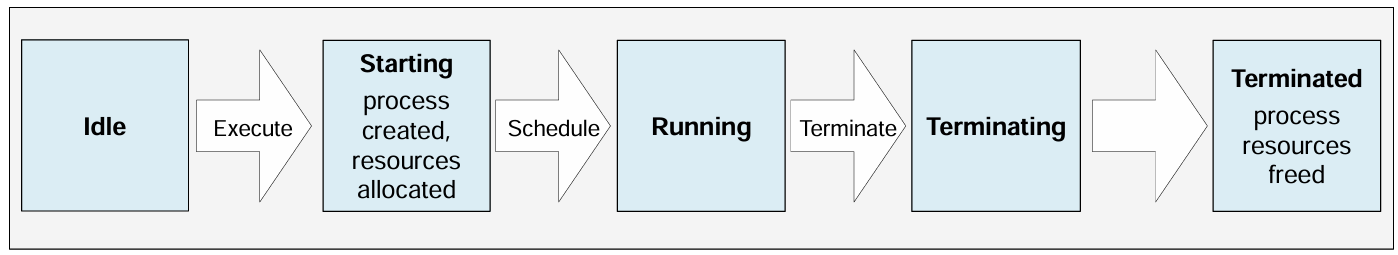
\includegraphics[width=0.9\textwidth]{Images/chapter2/em_processstate.png}
    \vspace{0.5cm}
    \caption{Process State \cite{autosar_exec_mgmt}}
    \label{fig:em_processstate}
\end{figure}

Strict error handling is enforced throughout this lifecycle. If a process exits with a non-zero status or terminates unexpectedly while running, Execution Management logs the event, flags the associated Function Group with an "Undefined Function Group State," and reports an \texttt{ExecutionError} to trigger higher-level recovery actions.

% \subsubsection{State Interaction}

% The operational behavior of the AUTOSAR Adaptive Platform is defined by the synchronization of three distinct state layers. State Interaction describes the handshake mechanism where high-level vehicle decisions (State Management) translate into low-level process lifecycles (Execution Management), which are then confirmed by the applications themselves (Process). This multi-layered approach ensures that the "Machine" does not merely start processes blindly, but confirms they are fully initialized and functionally ready before declaring a state transition complete.

% \begin{figure}[h]
%     \centering
%     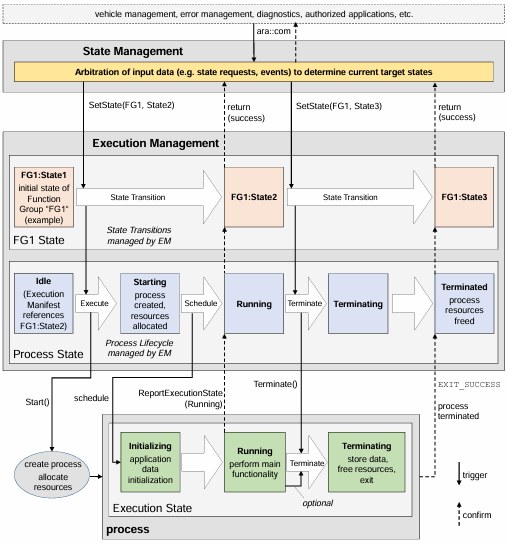
\includegraphics[width=0.9\textwidth]{Images/chapter2/em_stateinteraction.png}
%     \vspace{0.5cm}
%     \caption{State Interaction \cite{autosar_exec_mgmt}}
%     \label{fig:state_interaction}
% \end{figure}

% \paragraph*{Hierarchy of States:}
% To understand the interaction, one must first distinguish the three perspectives regarding "state" within the platform. {Function Group States (The Request)} are defined in the Manifest and controlled by State Management (SM). These represent a coherent mode of operation for a specific set of functionality (e.g., MachineFG in state Startup or a user-defined Function Group in state Run). SM determines what needs to run based on vehicle-wide events. {Process States (The Manager's View)} are maintained internally by Execution Management (EM). These track the lifecycle of a specific process instance (e.g., Idle, Starting, Running, Terminating, Terminated). EM uses these states to manage timeouts and resolve dependencies between applications. {Execution States (The Application's View)} are the internal lifecycle visible to the process itself (e.g., Initializing, Running, Terminating). The process reports these states to EM to confirm its readiness.

% \paragraph*{The Interaction Workflow:}
% The interaction is a cascading flow of triggers and confirmations. It typically begins with a request from State Management and ends with a confirmation from Execution Management, contingent upon the behavior of the individual processes.

% The process initiates with {The Trigger}, where State Management acts as the arbitrator. It analyzes input data (such as ignition signals or diagnostic requests) and determines that a Function Group (e.g., FG1) must transition to a specific state (e.g., State2). SM sends a \texttt{SetState(FG1, State2)} request to Execution Management. If FG1 is already in transition, EM will cancel the previous transition and reject the new request with \texttt{kCancelled} to ensure deterministic behavior.

% Upon receiving the request, Execution Management performs {Process Identification} by consulting the Execution Manifests to identify which processes are mapped to FG1:State2. Processes not currently running but required for State2 are queued for startup, while processes currently running but not required for State2 are queued for termination.

% For a process that needs to start, the {Startup and Initialization} phase begins. EM instructs the Operating System to create the process and allocate resources. Simultaneously, EM moves its internal tracking of the process to the Starting Process State. The OS creates the process entry point (\texttt{main}), and the process enters its own Execution State of Initializing. During this phase, the application loads configurations, initializes memory, and prepares to offer services.

% The critical point of interaction is {The Handshake}. EM considers the process to be Starting, but it does not assume the process is functional yet. Once the application completes its initialization and is ready to serve other components, it must explicitly call the API: \texttt{ara::exec::ExecutionClient::ReportExecutionState(kRunning)}. EM receives this call and updates its internal Process State from Starting to Running. If the process is a Non-reporting Process (legacy or simple applications), EM skips the handshake and assumes the process is Running immediately after the OS creates it.

% Finally, {Dependency Resolution and Confirmation} occurs. The interaction involves groups of processes; if Process B depends on Process A, EM will not start Process B until Process A has successfully performed the "Handshake" (reported \texttt{kRunning}). Only once all required processes for FG1:State2 have reported \texttt{kRunning} (and all unneeded processes have terminated), EM returns success to the original \texttt{SetState} call from State Management.

% \paragraph*{Deviations and Error Interactions:}
% The State Interaction mechanism is designed to be robust against failures. The interaction changes significantly if processes fail to participate correctly.

% In the case of a {Timeout on Startup}, if a process hangs during initialization and fails to call \texttt{ReportExecutionState(kRunning)} within a configured timeout, EM detects the timeout. EM attempts to restart the process up to a configured limit (\texttt{numberOfRestartAttempts}). If it still fails, EM aborts the Function Group transition, sets the state to Undefined, and reports an error to SM.

% An {Unexpected Termination} occurs if a process crashes (exits with a non-zero status) or exits without being asked (self-termination without permission) while EM thinks it should be running. EM detects the exit via OS mechanisms (e.g., \texttt{waitpid}) and reports this as an Unexpected Termination. The Function Group State is set to Undefined, and a callback is triggered in SM to handle the failure (e.g., by entering a Safe State).

% When transitioning out of a state, the {Termination Interaction} reverses. EM sends a \texttt{SIGTERM} signal to the process and updates the internal state to Terminating. The process receives the signal, saves data, cleans up resources, and exits with \texttt{EXIT\_SUCCESS}. EM detects the successful exit and moves the internal state to Terminated. If the process refuses to exit within a timeout, EM is authorized to use \texttt{SIGKILL} to enforce the state change.


% \paragraph*{Summary of Key Dependencies:}
% The State Interaction model relies on strict dependencies to ensure safety and determinism. {Manifest Verification} ensures EM will only execute processes explicitly mapped to the active Function Group State in the Manifest. The {Separation of Concerns} means the process does not know about the "Machine State" or "Function Group," only that it is Initializing or Running; EM acts as the bridge. Furthermore, there are {No Hidden Dependencies}: dependencies between processes must be resolved within the same Function Group State. A process in Group A cannot block a process in Group B via Execution Management mechanisms; such logic must be handled by State Management.

% By decoupling the request (SM) from the execution (EM) and the confirmation (Process), the Adaptive Platform ensures that the system state is always a verified reflection of the running software, rather than just a target configuration.


\subsubsection{State Interaction}

The operational behavior of the AUTOSAR Adaptive Platform relies on synchronizing three distinct state layers. This ``State Interaction'' ensures that the platform does not blindly start processes. Instead, it requires confirmation that applications are fully initialized and ready to run before declaring a state transition complete.

\begin{figure}[h]
    \centering
    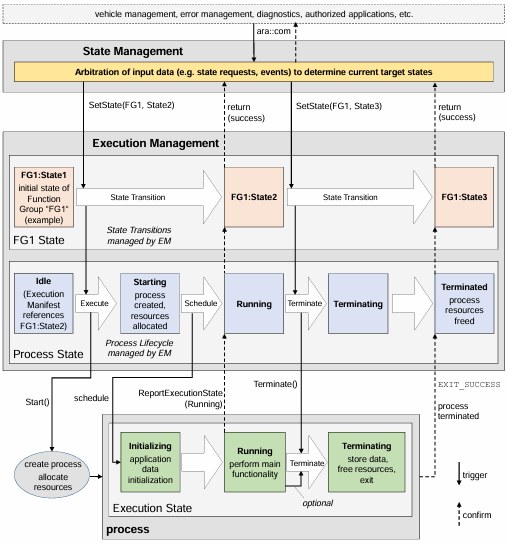
\includegraphics[width=0.9\textwidth]{Images/chapter2/em_stateinteraction.png}
    \vspace{0.5cm}
    \caption{State Interaction \cite{autosar_exec_mgmt}}
    \label{fig:state_interaction}
\end{figure}

\paragraph*{Understanding the Diagram Workflow:}
As illustrated in Figure \ref{fig:state_interaction}, the interaction between the layers acts as a clear chain of triggers (requests) and confirmations. To understand this, we must look at three distinct perspectives:

\begin{itemize}
    \item \textbf{State Management (The Requestor):} State Management (SM) acts as the arbitrator. Based on vehicle events, it decides the target state and triggers the workflow by sending a \texttt{SetState} request (e.g., \texttt{SetState(FG1, State2)}) to Execution Management.
    \item \textbf{Execution Management (The Manager):} Execution Management (EM) receives the request and manages the state transition. For processes that need to start, it moves its internal Process State from \texttt{Idle} to \texttt{Starting}. It then interacts with the Operating System to create the process and allocate resources.
    \item \textbf{The Process (The Application):} Once scheduled, the process enters its internal \texttt{Initializing} state to load data and set up services. Crucially, EM waits for a ``handshake.'' Once initialization is complete, the process explicitly sends a \texttt{ReportExecutionState(Running)} signal back to EM.
\end{itemize}

\paragraph*{Confirmation and Termination:}
After receiving this running confirmation, EM updates its internal state to \texttt{Running} and finally returns a ``success'' confirmation back to State Management, completing the startup workflow. 

The termination process follows a similar, reversed logic. When SM requests a new state that requires shutting down an application, EM sends a \texttt{Terminate()} trigger. The process enters the \texttt{Terminating} state to safely store data and free resources before exiting with an \texttt{EXIT\_SUCCESS} signal. EM then marks the process as \texttt{Terminated} and confirms the success with SM.

\paragraph*{Summary:}
Ultimately, this interaction model relies on strict rules and clear separation of responsibilities. By separating the request (from SM), the execution (by EM), and the confirmation (from the Process), the platform guarantees that the system's state accurately reflects the actual running software.


% \subsection{Communication Management (\texttt{ara::com})}

% Communication Management is responsible for all aspects of communication between applications in a distributed real-time embedded environment, acting as the middleware that abstracts network details from the application logic. It facilitates Service-Oriented Communication (SoC) by providing a standardized API that allows Adaptive Applications to offer or consume services without knowledge of the underlying transport mechanisms. ara::com establishes communication paths between partners at runtime, relying on the Service Registry to broker the connection between Service Providers and Service Consumers, whether they reside on the same machine or across the vehicle network.

% It manages the exchange of data through the Proxy/Skeleton architectural pattern, where the Service Skeleton connects the provider's implementation to the middleware, and the Service Proxy provides the consumer with a local C++ interface to access the remote service. For this system, ara::com utilizes the SOME/IP network binding to handle the specific requirements of the transport layer. This binding is responsible for discovering services on the network (Service Discovery) and serializing application data—specifically Methods, Events, and Fields—into the SOME/IP wire format. This separation of the Language Binding (C++ API) from the Network Binding ensures that the application code remains portable and independent of the specific protocol configuration defined in the Service Instance Manifests.

% To ensure secure and reliable operation, Communication Management enforces strict access control and data integrity. It integrates with Identity and Access Management (IAM) to verify that a requesting application process possesses the required Grants to access a specific Service Interface, dropping unauthorized requests at the middleware level. Furthermore, ara::com supports End-to-End (E2E) protection, which safeguards the transmission of events and methods against faults such as data corruption or loss, ensuring that safety-critical data exchanged via SOME/IP remains valid upon reception.

\subsection{Communication Management (\texttt{ara::com})}

Communication Management (\texttt{ara::com}) acts as the middleware that handles all communication between applications in a real-time embedded environment. It enables Service-Oriented Communication (SoC) by providing a standardized API, allowing applications to offer or consume services without needing to know the complex underlying network details. At runtime, it uses a Service Registry to connect Service Providers with Service Consumers across the vehicle network.

The system exchanges data using the Proxy/Skeleton pattern. The Service Skeleton connects the provider to the middleware, while the Service Proxy gives the consumer a local C++ interface to access remote services. To handle data transport, \texttt{ara::com} utilizes network bindings like SOME/IP and DDS (Data Distribution Service). These bindings manage service discovery and convert application data—such as Methods, Events, and Fields—into the appropriate network format. By separating the C++ language API from the network protocols, the application code remains flexible and easy to port.

Finally, \texttt{ara::com} ensures secure and reliable data transfer. It works with Identity and Access Management (IAM) to verify that applications have the correct permissions before allowing access to a service. Additionally, it supports End-to-End (E2E) protection to prevent data loss or corruption, guaranteeing that safety-critical information exchanged via SOME/IP or DDS remains accurate and secure.


\subsubsection{Block View Diagram}

\begin{figure}[h]
    \centering
    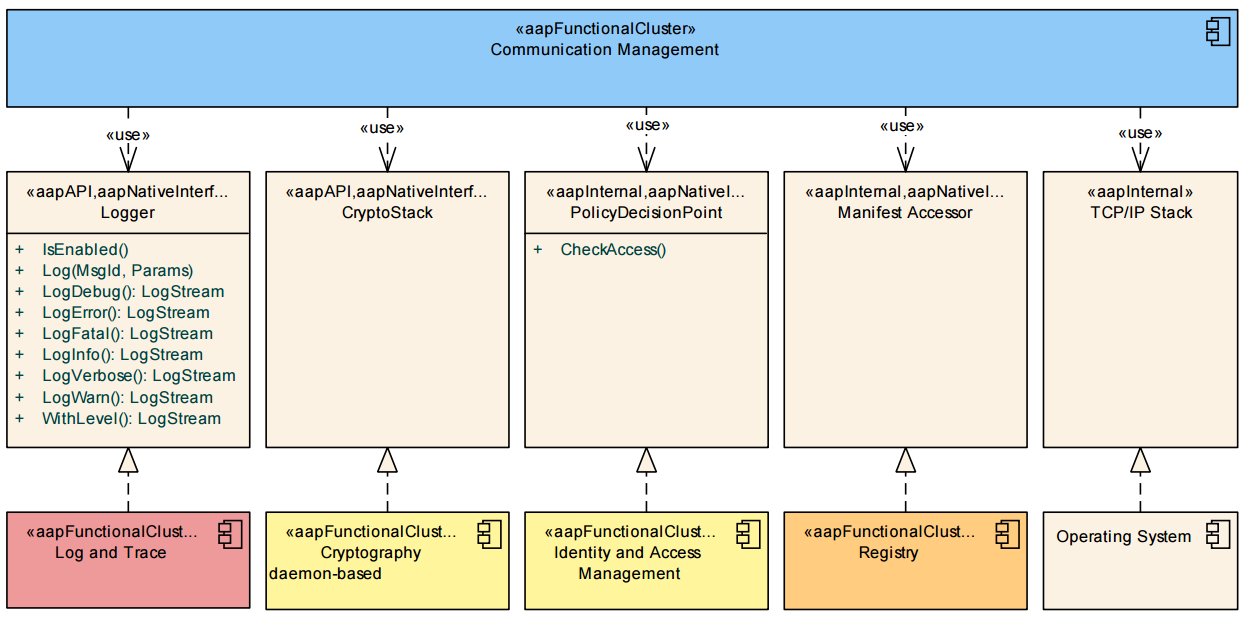
\includegraphics[width=1\textwidth]{Images/chapter2/com_required.png}
    \vspace{0.5cm}
    \caption{Required Interfaces of Communication Management \cite{autosar_sw_arch}}
    \label{fig:CommunicationManagementRequiredInterfaces}
\end{figure}

\textbf{Required Interfaces:} \begin{itemize} 
    \item \texttt{Cryptography::CryptoStack}: Communication Management shall use this interface to establish encrypted connections and generate / verify checksums (MAC).   
    \item \texttt{EventReporter}: This interface should be used to report security events. 
    \item \texttt{FVM}: Communication Management shall use this interface to get freshness values. 
    \item \texttt{Identity and Access Management::PolicyDecisionPoint}: Communication Management shall use this interface to check access to \texttt{ara::com} service methods, fields, and events. 
    \item \texttt{Log and Trace::Logger}: Communication Management shall use this interface to log standardized messages. 
    \item \texttt{Manifest Accessor}: Communication Management shall use this interface to read service information from the Manifests. 
    \item \texttt{Operating System::OperatingSystemInterface}: Communication Management should use this interface to create and control Threads used by the implementation. 
    \item \texttt{TCP/IP Stack}: Communication Management shall use this interface to establish and control TCP/IP-based network connections. 
\end{itemize}

\subsubsection{\texttt{ara::com} Responsibilities}

Communication Management (\texttt{ara::com}) is responsible for all aspects of communication between applications in a distributed, real-time embedded environment. Its primary design goal is to abstract the mechanisms used for finding and connecting communication partners, enabling developers to focus on application logic rather than data transport details. This cluster facilitates {Service-Oriented Communication (SOC)} between Adaptive Applications, handling both intra-machine (IPC) and inter-machine communication with other platforms, Classic AUTOSAR ECUs, or non-AUTOSAR entities.

To realize this, \texttt{ara::com} manages services defined by Events, Methods, and Fields using a {Service Registry}. This registry acts as a broker where applications register their Provided Services. Consuming applications utilize {Service Discovery} to locate these services at runtime. This allows for dynamic communication patterns where partners are identified during execution, though static configuration is also supported.

The architecture decouples software from transport technologies via two layers. The {Language Binding} maps abstract service definitions to specific C++ interfaces, generating Proxy classes for clients and Skeleton classes for providers to ensure type safety. The {Network Binding} handles data serialization for various protocols (e.g., SOME/IP, DDS, IPC) and manages transmission. This ensures application portability independent of the deployment scenario.

Beyond standard services, \texttt{ara::com} handles {Raw Binary Data Streams} for interacting with external sensors or systems providing untyped data. A dedicated API (\texttt{ara::com::raw}) allows applications to establish direct client/server connections over protocols like TCP/IP, bypassing the overhead of service serialization.

Finally, the module is critical for {Safety and Security}. It integrates End-to-End (E2E) protection to verify data integrity against communication faults. For security, it enforces access control by interacting with Identity and Access Management (IAM) to verify sender identity and permissions. Secure channels are managed using protocols like TLS, DTLS, and SecOC to ensure confidentiality and authenticity.

% \subsubsection{Service Registry and Discovery}

% In the Service-Oriented Communication (SOC) architecture of the AUTOSAR Adaptive Platform, the Service Registry and Service Discovery mechanisms are critical components that decouple application software from the underlying network topology.

% \paragraph*{The Service Registry:}
% The Service Registry functions as a central brokering instance within the \texttt{ara::com} infrastructure. Its primary responsibility is to maintain a dynamic directory of available services, abstracting the low-level details of network addresses and transport protocols from the application developers. When an Adaptive Application offers a service, it registers this service with the Service Registry, thereby making the functionality visible to other applications within the system. Conversely, when a client application requires a specific service, it does not connect to a hard-coded IP address; instead, it queries the Service Registry to locate the desired service instance. This abstraction allows the Communication Management logic to transparently route requests, whether the service resides in the same process, on the same machine, or on a remote ECU connected via Ethernet. In the physical architecture of the platform, the Registry is categorized under the Configuration functional clusters. It interacts internally with other clusters, such as Identity and Access Management and Communication Management, often utilizing the Manifest Accessor interface to validate service configurations against the system design.

% \paragraph*{The Service Discovery Process:}
% Service Discovery is the dynamic run-time process governed by \texttt{ara::com} to match Service Providers with Service Consumers based on the entries in the Service Registry. This mechanism allows the system to establish communication paths at runtime, supporting dynamic architectures where the availability of services may change or where the specific location of a service is not known at compile time. The discovery process begins with the Service Provider. When an application has initialized a service skeleton, it calls the \texttt{OfferService()} API. This action triggers the underlying network binding to announce the service's availability to the network. On the Service Consumer side, the application utilizes the \texttt{FindService()} or \texttt{StartFindService()} APIs. The \texttt{ara::com} runtime then queries the registry (or listens to network announcements) to find matching service instances. If matches are found, the runtime returns a list of handles (\texttt{ServiceHandleContainer}) to the consumer, which can then be used to instantiate a Proxy and begin data exchange.

% \begin{figure}[h]
%     \centering
%     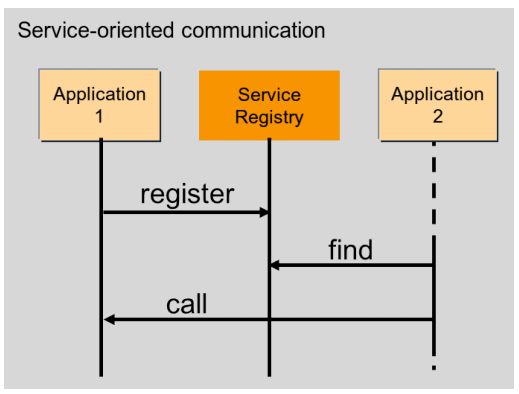
\includegraphics[width=0.5\textwidth]{Images/chapter2/com_soc.png}
%     \vspace{0.5cm}
%     \caption{Service-oriented communication \cite{autosar_com_mgmt}}
%     \label{fig:com_soc}
% \end{figure}

% \paragraph*{Protocol-Specific Implementation:}
% While the \texttt{ara::com} API abstracts the discovery process for the developer, the underlying behavior varies significantly depending on the network binding configuration.
% \begin{itemize}
%     \item \textbf{SOME/IP Service Discovery:} When using the SOME/IP binding, offering a service triggers the SOME/IP Service Discovery Protocol. This involves sending OfferService messages, which may be multicast or unicast depending on the configuration. The process includes configurable phases, such as an "Initial Wait Phase" and a "Repetition Phase," to ensure robust announcement on the network. Similarly, finding a service triggers FindService messages. The system also supports SubscribeEventgroup messages to manage dynamic subscriptions to specific data feeds within a service.

%     \item \textbf{SOME/IP Service Discovery:} When using the SOME/IP binding, offering a service triggers the SOME/IP Service Discovery Protocol. This involves sending OfferService messages, which may be multicast or unicast depending on the configuration. The process includes configurable phases, such as an "Initial Wait Phase" and a "Repetition Phase," to ensure robust announcement on the network. Similarly, finding a service triggers FindService messages. The system also supports SubscribeEventgroup messages to manage dynamic subscriptions to specific data feeds within a service.

%     \item \textbf{DDS Service Discovery:} The Data Distribution Service (DDS) binding offers two distinct discovery protocols configurable via the manifest. The first is {DomainParticipantUserDataQos}, which leverages the USER\_DATA QoS policy of DDS Domain Participants. The system encodes service IDs and instance IDs into the user data of the participant discovery messages. This approach is efficient as it uses the built-in DDS discovery traffic without creating extra entities. Alternatively, the system can use {Topic-Based Discovery}, employing a dedicated DDS Topic (e.g., \texttt{ara.com://services/discovery}) to publish service announcements. While this requires creating additional DataWriters and DataReaders, it enhances interoperability and supports advanced features like persistence and routing.

%     \item \textbf{Signal-Based Static Discovery:} For legacy compatibility or static configurations (e.g., interacting with simple sensors), the platform supports a static binding. In this case, \texttt{FindService} immediately returns a pre-configured handle containing static socket information (IP and Port) without performing active network discovery.
% \end{itemize}

% \paragraph*{Service Contract Versioning:}
% Service Discovery is not merely about finding a name; it also ensures compatibility. The platform supports Service Contract Versioning, where a service interface is defined by a Major and Minor version. During the discovery process, \texttt{ara::com} evaluates the version of the offered service against the version requested by the consumer. A connection is generally established only if the versions are backward-compatible (e.g., same Major version, offered Minor version greater than or equal to requested Minor version).

% \begin{figure}[h]
%     \centering
%     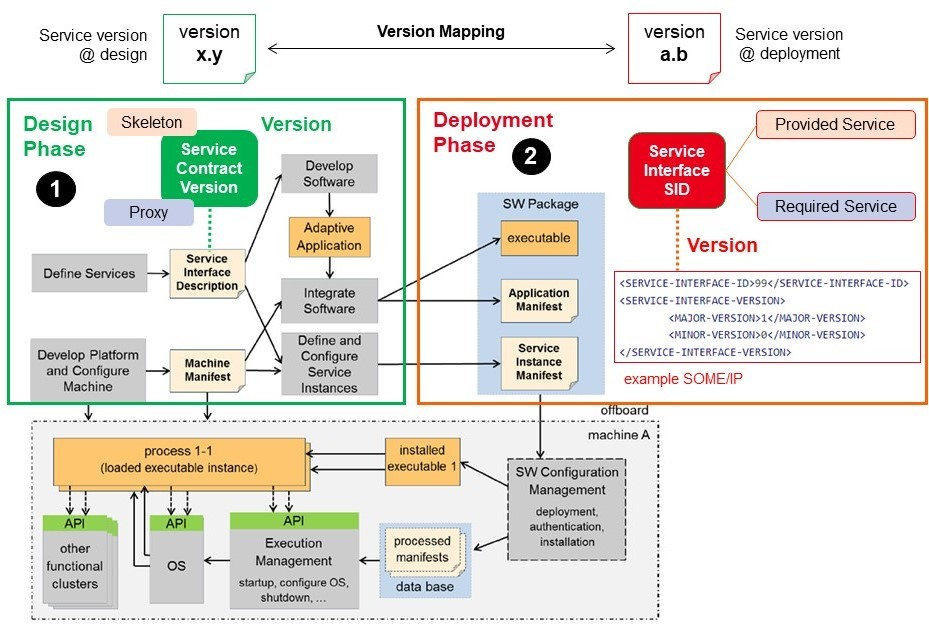
\includegraphics[width=0.9\textwidth]{Images/chapter2/com_servicecontract.jpg}
%     \vspace{0.5cm}
%     \caption{Service Contract Versioning flow \cite{autosar_com_mgmt}}
%     \label{fig:com_servicecontract}
% \end{figure}

\subsubsection{Service Registry and Discovery}

Within the \texttt{ara::com} Service-Oriented Communication (SOC) framework, the Service Registry and Service Discovery mechanisms decouple applications from the physical network topology. The Service Registry acts as a central broker, maintaining a dynamic directory of available services. This abstracts complex network addresses and transport protocols from developers, allowing the middleware to transparently route requests whether services reside locally or on a remote ECU. 

Service Discovery is the runtime process that matches Service Providers with Consumers. Providers register their capabilities via the \texttt{OfferService()} API, triggering network announcements. Conversely, consumers use the \texttt{FindService()} API to query the registry. Upon finding a match, the runtime returns a \texttt{ServiceHandleContainer}, which the consumer uses to instantiate a Proxy and initiate communication.

\begin{figure}[h]
    \centering
    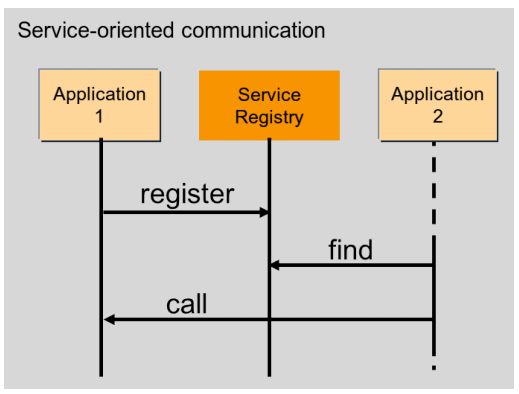
\includegraphics[width=0.5\textwidth]{Images/chapter2/com_soc.png}
    \vspace{0.5cm}
    \caption{Service-oriented communication \cite{autosar_com_mgmt}}
    \label{fig:com_soc}
\end{figure}

\paragraph*{Protocol-Specific Discovery \& Versioning:}
While the \texttt{ara::com} API abstracts the process, the underlying discovery mechanism varies by network binding:
\begin{itemize}
    \item \textbf{SOME/IP:} Triggers the SOME/IP Service Discovery Protocol, utilizing configurable \textit{OfferService} and \textit{FindService} multicast/unicast messages, alongside \textit{SubscribeEventgroup} for dynamic data feeds.
    \item \textbf{DDS:} Configurable via either \textit{DomainParticipantUserDataQos} (embedding service IDs efficiently into participant discovery traffic) or \textit{Topic-Based Discovery} (using a dedicated DDS topic for service announcements).
    \item \textbf{Static Discovery:} For legacy systems, \texttt{FindService} immediately returns a pre-configured static socket handle (IP/Port) without active network discovery.
\end{itemize}

Additionally, discovery enforces \textbf{Service Contract Versioning} (Major and Minor versions). A connection is successfully established only if the provider's version is backward-compatible with the consumer's request.

\begin{figure}[h]
    \centering
    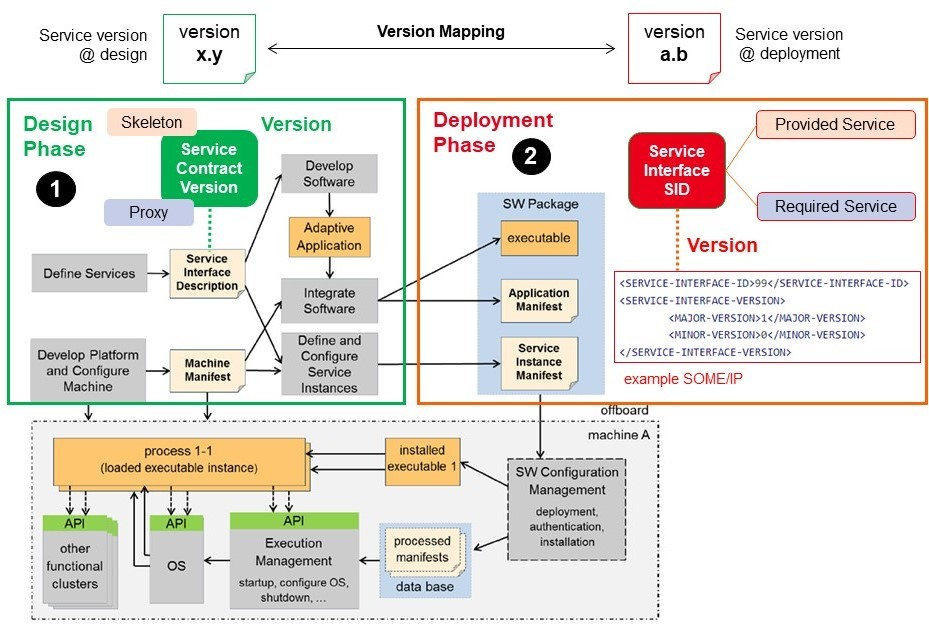
\includegraphics[width=0.9\textwidth]{Images/chapter2/com_servicecontract.jpg}
    \vspace{0.5cm}
    \caption{Service Contract Versioning flow \cite{autosar_com_mgmt}}
    \label{fig:com_servicecontract}
\end{figure}

% \subsubsection{Proxy/Skeleton Management}

% The Communication Management functional cluster in the AUTOSAR Adaptive Platform utilizes the Proxy/Skeleton design pattern to realize Service Oriented Communication. This architecture abstracts the underlying communication mechanisms, allowing applications to communicate regardless of whether the service resides in the same process, on a different process, or on a remote machine. The C++ Language Binding provides an object-oriented mapping of the services defined in the AUTOSAR meta-model, where a generator tool creates C++ classes containing type-safe representations of methods, events, and fields.

% On the client side, the {Service Proxy} acts as the local representative of a potentially remote service. These generated classes, known as Service Requester Proxies, can be used directly by the client application to access the service. To utilize a proxy, the client application must first identify a specific service instance using the \texttt{FindService} API, which returns handles that are passed to the proxy constructor to create a valid instance. The proxy provides mechanisms for calling service methods either synchronously, which blocks the caller until a result is returned, or asynchronously, where the function returns immediately and the result is retrieved later via \texttt{ara::core::Future}.

% On the server side, the {Service Skeleton} connects the user-provided service implementation to the middleware transport infrastructure. These generated classes are called Service Provider Skeletons and function as abstract base classes. A service implementation must derive from the generated skeleton class and implement the respective functionality. The skeleton provides specific methods to control the visibility of the service, such as \texttt{OfferService} to make the service available to applications and \texttt{StopOfferService} to stop offering it. Additionally, the architecture supports "Multi-Binding," allowing a single proxy or skeleton class to utilize different technical transport layers or protocols for communication.

% \begin{figure}[h]
%     \centering
%     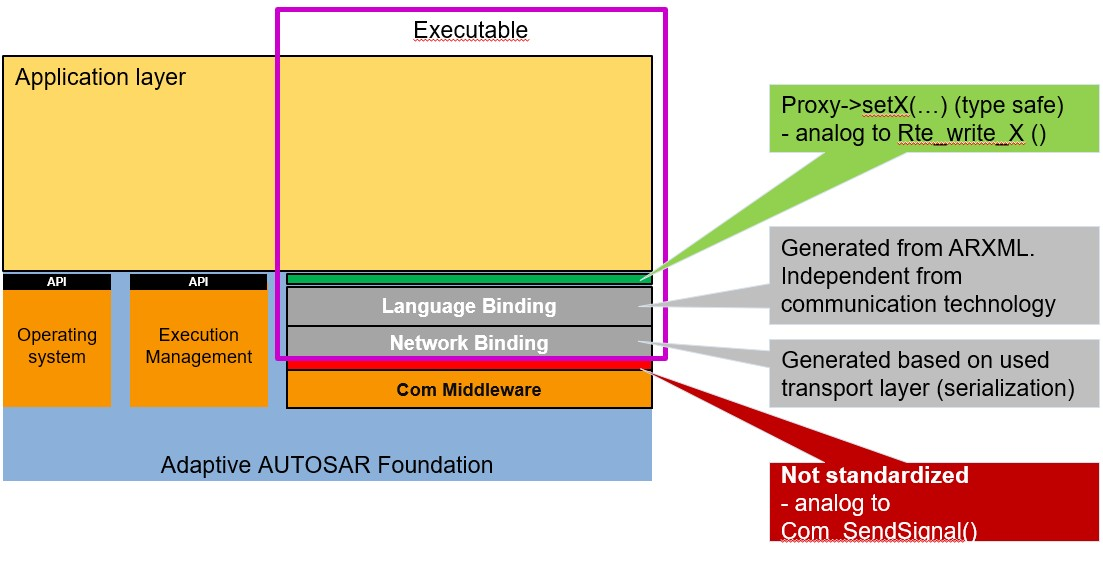
\includegraphics[width=1\textwidth]{Images/chapter2/com_networkbinding.jpg}
%     \vspace{0.5cm}
%     \caption{Example Language and Network Binding \cite{autosar_com_mgmt}}
%     \label{fig:com_languagebinding}
% \end{figure}

% The figure \ref{fig:com_languagebinding} illustrates the relationship between the Application layer (where Proxy calls occur), the generated Language Binding, and the Network Binding.

\subsubsection{Proxy/Skeleton Management}

The \texttt{ara::com} functional cluster uses the Proxy/Skeleton design pattern to enable Service-Oriented Communication. This architecture hides the underlying network details, allowing applications to communicate seamlessly, whether the service is on the same machine or across the network. A generator tool creates C++ classes that provide type-safe representations of methods, events, and fields based on the AUTOSAR meta-model.

\paragraph*{Service Skeleton (Provider):}
On the server side, the Service Skeleton connects the user's implementation to the middleware. The application creates an instance of the skeleton and calls \texttt{Start()} (or \texttt{OfferService()}) to make it available to others. When data needs to be sent, it triggers an event.

For example, a SOME/IP Provider might offer a sensor service like this:
\begin{lstlisting}[language=C++]
// SOME/IP Provider Initialization
m_Sensorv2 = std::make_unique<providersensor::rootswcomponent::port::Sensorv2>();
m_Sensorv2->Start(); // Offer service to the network

// Sending data via SOME/IP Event
m_Sensorv2->SendEventEvent_RequestDataTriggered(m_sensorData);
\end{lstlisting}

Similarly, a DDS Provider follows the exact same pattern, proving the abstraction of \texttt{ara::com}:
\begin{lstlisting}[language=C++]
// DDS Provider Initialization
m_PPort0 = std::make_unique<providersensor::aa::port::PPort0>();
m_PPort0->Start(); // Offer service over DDS

// Sending data via DDS Event
m_PPort0->SendEventimageDataEventTriggered(m_sensorData);
\end{lstlisting}

\paragraph*{Service Proxy (Client):}
On the client side, the Service Proxy acts as a local representative of the remote service. The client application uses the proxy to register handlers for incoming events or to call methods (synchronously or asynchronously).

For example, a SOME/IP Client registers a callback to handle incoming sensor data:
\begin{lstlisting}[language=C++]
// SOME/IP Client Registration
m_Sensorv2 = std::make_unique<clientsensor::rootswcomponent::port::Sensorv2>();
m_Sensorv2->RegistEventHandlerEvent_RequestData(
    [this](const sensor::transv2::proxy::events::Event_RequestData::SampleType& data) {
        // Handle received data
    }
);
m_Sensorv2->Start(); // Start listening
\end{lstlisting}

A DDS Client handles data similarly, registering an event handler for the specific DDS topic:
\begin{lstlisting}[language=C++]
// DDS Client Registration
m_RPort0 = std::make_unique<clientsensor::aa::port::RPort0>();
m_RPort0->RegistEventHandlerimageDataEvent(
    [this](const sensorCam::proxy::events::imageDataEvent::SampleType& data) {
        // Parse and process received image data
    }
);
m_RPort0->Start(); // Start listening
\end{lstlisting}

\paragraph*{Multi-Binding and Abstraction:}
As seen in the examples, whether the system uses SOME/IP or DDS, the application code structure remains nearly identical. This demonstrates the power of ``Multi-Binding,'' where a single proxy or skeleton class can utilize different network protocols without requiring changes to the core application logic. 

\begin{figure}[h]
    \centering
    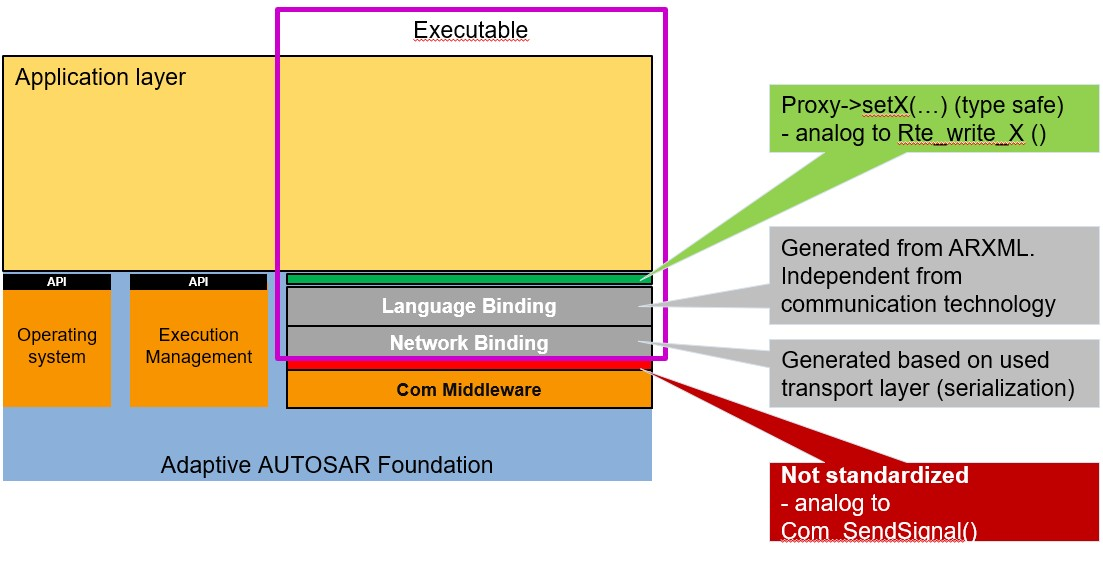
\includegraphics[width=1\textwidth]{Images/chapter2/com_networkbinding.jpg}
    \vspace{0.5cm}
    \caption{Example Language and Network Binding \cite{autosar_com_mgmt}}
    \label{fig:com_languagebinding}
\end{figure}

Figure \ref{fig:com_languagebinding} illustrates this relationship between the Application layer (where Proxy calls occur), the generated Language Binding, and the Network Binding.

\subsubsection{Access Control}

The access control mechanism within the Communication Management (\texttt{ara::com}) functional cluster is designed to restrict the interaction capabilities of both local applications and remote subjects, such as external ECUs, thereby limiting potential damage from compromised entities. This security feature integrates with the {Identity and Access Management (IAM)} framework, where \texttt{ara::com} acts as a {Policy Enforcement Point (PEP)} that queries the IAM {Policy Decision Point (PDP)} to authorize requests based on configured policies. Access permissions are modeled using \texttt{ComGrant} elements; if a grant references a \texttt{remoteSubject}, it applies to identified remote entities, otherwise, it applies to local processes based on their service instance to port prototype mappings. The enforcement of these rules is controlled by the \texttt{IamModuleInstantiation} configuration, which includes specific switches (\texttt{localComAccessControlEnabled} and \texttt{remoteAccessControlEnabled}) to independently activate access control for local processes and remote subjects.

For local applications, access control enforcement occurs at specific API interaction points. When an application attempts to offer a service via a \texttt{ServiceSkeleton} or find a service via a \texttt{ServiceProxy}, the framework checks for \texttt{ComOfferServiceGrant} or \texttt{ComFindServiceGrant} respectively; failure to possess these grants results in a \texttt{kGrantEnforcementError} returned to the application. Similarly, invoking service methods requires a \texttt{ComMethodGrant}, and unauthorized attempts will return a \texttt{kGrantEnforcementError} in the \texttt{Future} result of the method call. In contrast, unauthorized attempts to send or subscribe to events (requiring \texttt{ComEventGrant}) or triggers are handled by silently dropping the data or subscription request without notifying the application.

For remote access control, the system must first authenticate the remote subject using properties from established TLS connections, IPsec associations, or IP addresses before applying the modeled grants to permit or deny operations such as executing methods or subscribing to events.

\begin{figure}[h]
    \centering
    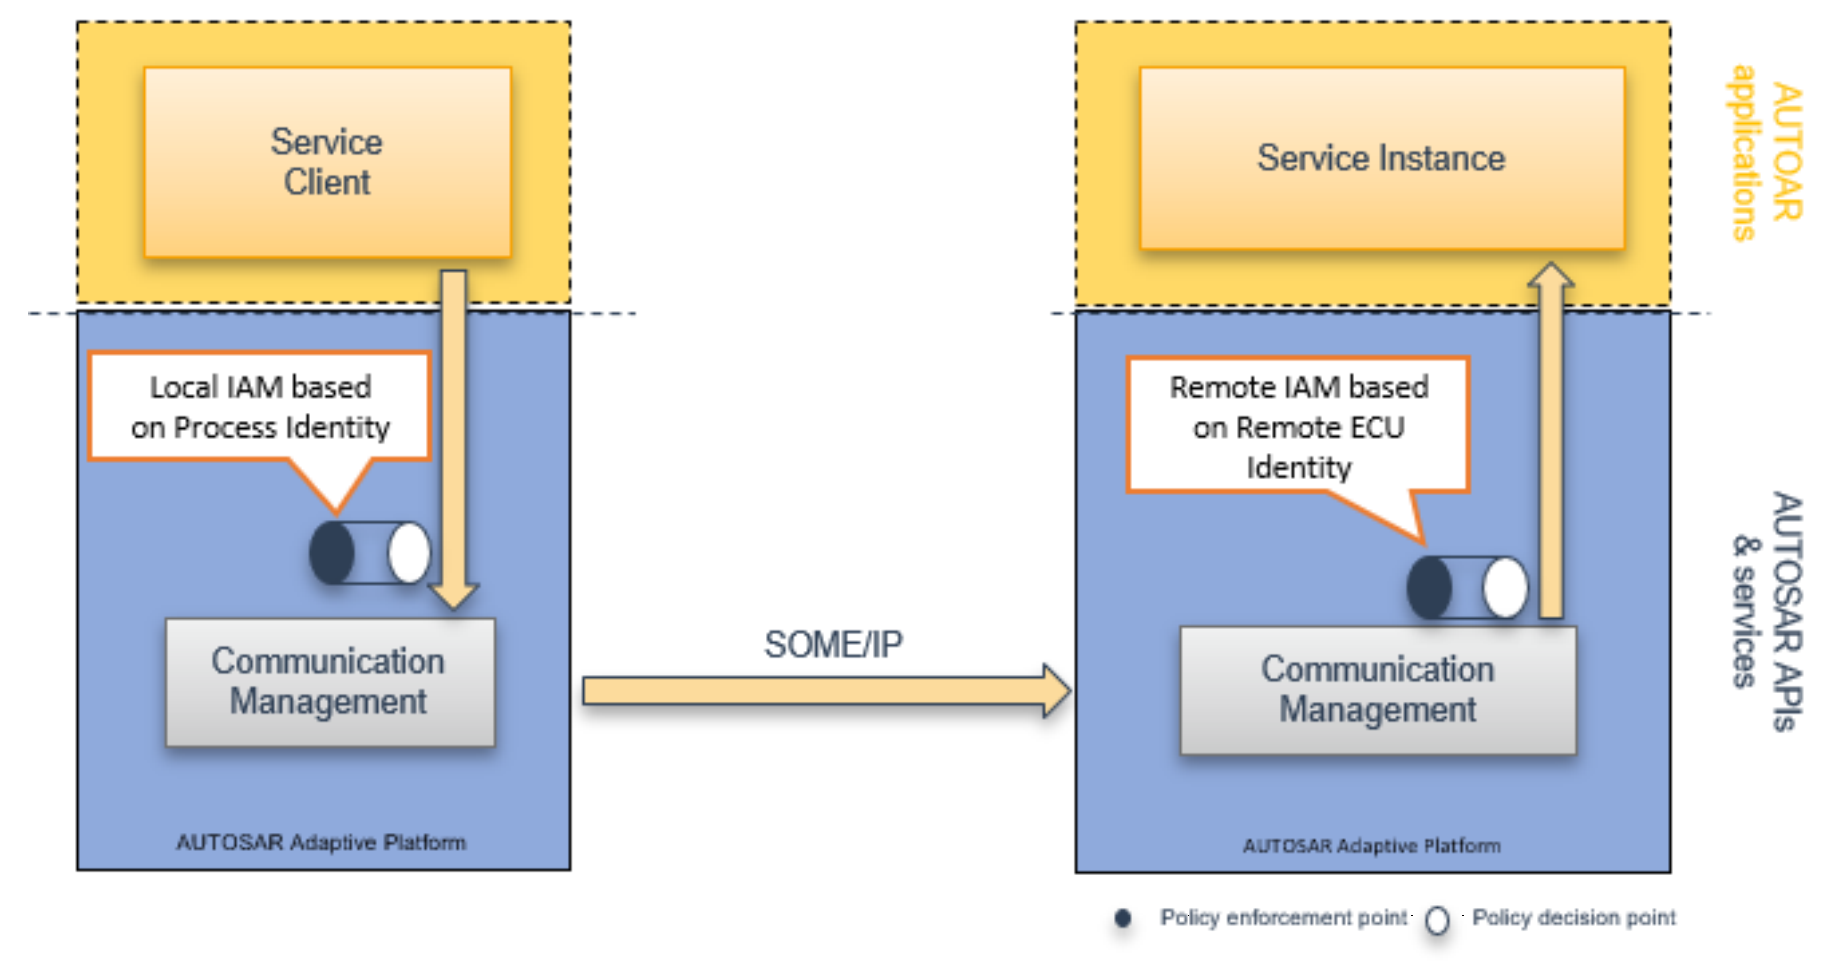
\includegraphics[width=1\textwidth]{Images/chapter2/com_iam.png}
    \vspace{0.5cm}
    \caption{Local and Remote Identity and Access Management \cite{autosar_com_mgmt}}
    \label{fig:com_iam}
\end{figure}



% \subsubsection{SOME/IP Protocol}

% See \ref{sec:someip_protocol} for more details.

% \subsection{Log and Trace (\texttt{ara::log})}

% The Log and Trace functional cluster (\texttt{ara::log}) is responsible for managing and instrumenting the logging features of the AUTOSAR Adaptive Platform, serving both development and production use cases. It provides standardized C++ interfaces that allow Adaptive Applications and other Functional Clusters to forward logging information to various ``sinks,'' such as a network communication bus, a file on the local file system, or a serial console. The module is designed to ensure platform stability by managing system resources and preventing data loss through internal buffering when high loads of trace information are generated simultaneously.

% To organize and filter the vast amount of data generated by modern vehicles, \texttt{ara::log} utilizes a strict identification and classification system. Every application instance is identified by a unique Application ID (\texttt{AppID}), while distinct logical groups within an application are distinguished using Context IDs (\texttt{CtxID}). Furthermore, every log message is assigned a specific severity level---ranging from \texttt{kFatal} and \texttt{kError} to \texttt{kDebug} and \texttt{kVerbose}. This allows the platform to be instrumented to only process and transmit messages above a configured threshold, enabling complex filtering and efficient fault detection without overloading the system.

% A critical architectural feature of \texttt{ara::log} is its support for two distinct classes of messages: Non-Modeled and Modeled. Non-Modeled messages (often called ``verbose'') contain all message arguments and text within the payload and are primarily used during development when flexibility is required. Conversely, Modeled messages (or ``non-verbose'') are optimized for production to minimize network bandwidth. In Modeled messages, static parts of the log (such as text strings) are stored in the application's ARXML manifest rather than being transmitted; only the message ID and dynamic arguments are sent over the network, allowing a viewer tool to reconstruct the full message using the model.

% Under the hood, \texttt{ara::log} relies on the standardized LT Protocol (Log and Trace Protocol) to pack logging information into a standardized delivery format, often utilizing the DLT (Diagnostic Log and Trace) backend implementation. This protocol is bus-agnostic and supports adding metadata, such as ECU IDs, to help clients sort and filter logs. Additionally, \texttt{ara::log} interacts with the Time Synchronization functional cluster (\texttt{ara::tsync}) to attach synchronized timestamps to messages, which is essential for correlating events across distributed systems.

% \begin{figure}[h]
%     \centering
%     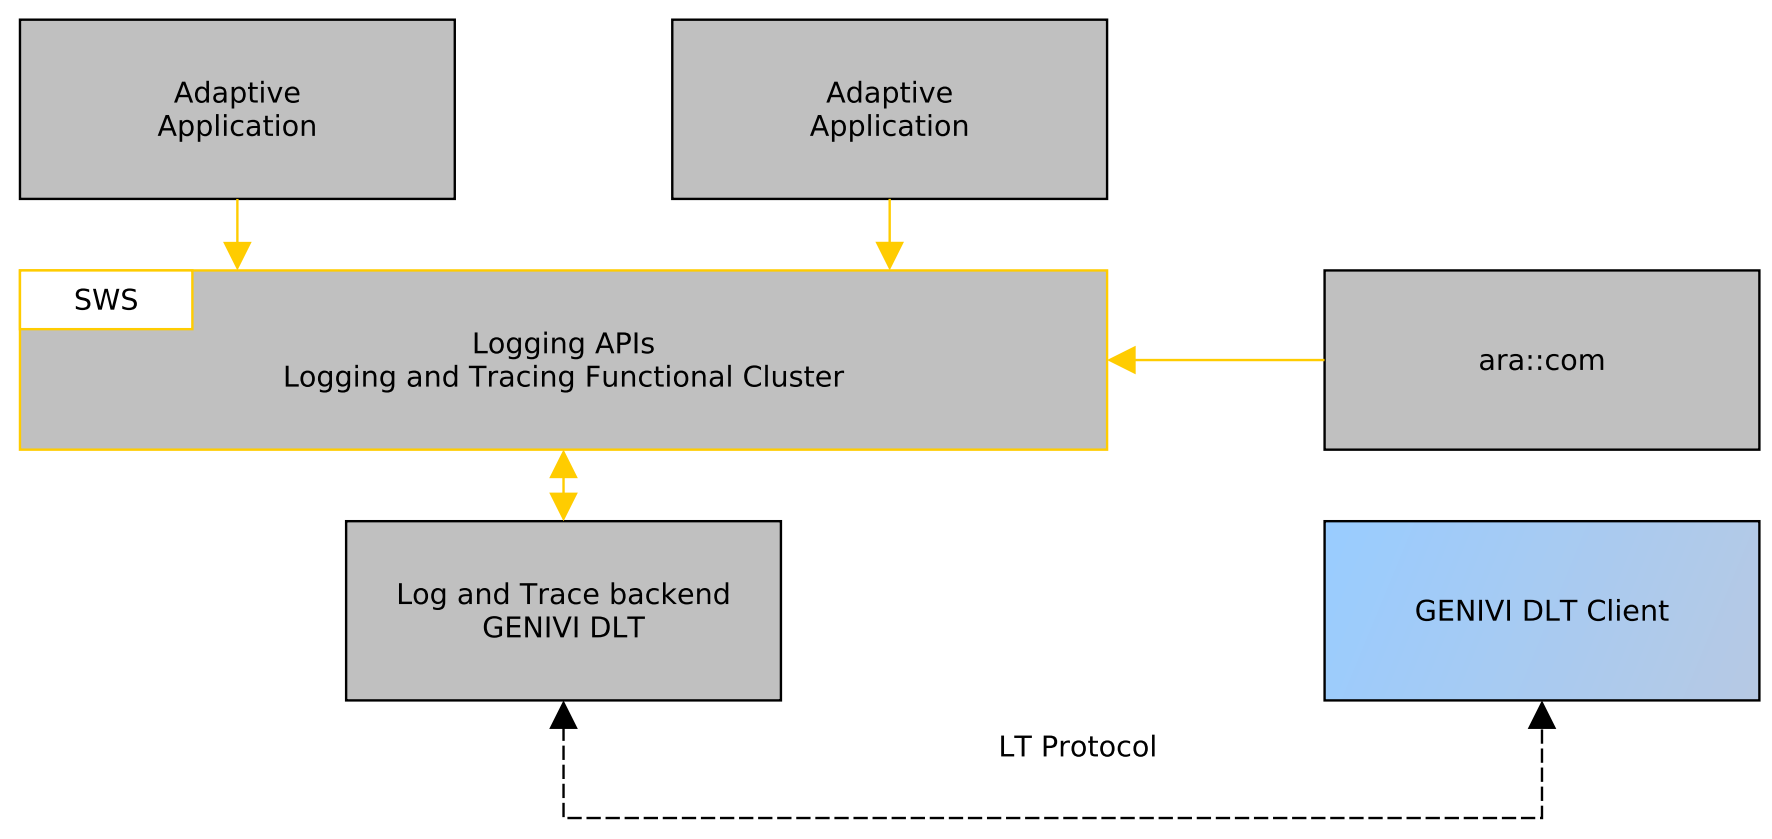
\includegraphics[width=1\textwidth]{Images/chapter2/log_arch.png}
%     \vspace{0.5cm}
%     \caption{Log and Trace Overview \cite{autosar_log_trace}}
%     \label{fig:log_arch}
% \end{figure}



% \subsubsection{Log Severity Levels}

% In the AUTOSAR Adaptive Platform, the Log and Trace functional cluster (\texttt{ara::log}) employs a standardized classification system known as ``severity levels'' to categorize every log message based on its importance. These levels are defined within the \texttt{ara::log::LogLevel} enumeration (based on \texttt{std::uint8\_t}) and serve a critical role in system stability by acting as a reporting filter. Each application process or logging context is configured with a specific log level threshold; the Logging framework only processes and transmits messages that have a severity equal to or higher than this configured threshold, while ignoring lower-priority messages. This filtering mechanism preserves CPU and memory resources by preventing the system from preparing and storing excessive data, such as verbose debug information, during normal production operation.

% \paragraph*{Defined Severity Levels:}
% The standard defines a specific hierarchy of severity levels, ranging from \texttt{0x00} to \texttt{0x06}, to cover various operational and development scenarios:

% \begin{table}[h]
%     \centering
%     \renewcommand{\arraystretch}{1.2}
%     \begin{tabular}{|l|c|p{9.5cm}|}
%         \hline
%         \textbf{Level Name} & \textbf{Value} & \textbf{Description} \\
%         \hline
%         \texttt{kOff} & \texttt{0x00} & This level indicates ``No logging'' and is used to disable log output entirely for a specific context or application. \\
%         \hline
%         \texttt{kFatal} & \texttt{0x01} & Represents a fatal error that is not recoverable. \\
%         \hline
%         \texttt{kError} & \texttt{0x02} & Denotes an error that has an impact on the correct functionality of the system. \\
%         \hline
%         \texttt{kWarn} & \texttt{0x03} & Used for warnings where correct behavior cannot be explicitly ensured. \\
%         \hline
%         \texttt{kInfo} & \texttt{0x04} & Provides high-level informational messages to understand the system flow. \\
%         \hline
%         \texttt{kDebug} & \texttt{0x05} & Contains detailed information intended specifically for programmers during development. \\
%         \hline
%         \texttt{kVerbose} & \texttt{0x06} & Represents the highest grade of information, providing extra-verbose debug messages. \\
%         \hline
%     \end{tabular}
%     \caption{Defined Log Severity Levels}
%     \label{tab:log_severity_levels}
% \end{table}

% \paragraph*{API Usage and Configuration:}
% To facilitate ease of use, the \texttt{ara::log::Logger} class provides dedicated API methods corresponding to each severity level, including \texttt{LogFatal()}, \texttt{LogError()}, \texttt{LogWarn()}, \texttt{LogInfo()}, \texttt{LogDebug()}, and \texttt{LogVerbose()}. Each of these methods returns a \texttt{LogStream} object pre-configured with the respective severity. Alternatively, if the severity needs to be determined programmatically at runtime, developers can use the \texttt{WithLevel()} method to pass the \texttt{LogLevel} as a parameter. To further optimize performance, the \texttt{IsEnabled()} function allows applications to check if a specific level is currently active before executing complex code to prepare log arguments, ensuring that resources are not wasted on messages that will eventually be discarded. The default log level is initially defined in the application execution manifest but can be overridden per context and adjusted dynamically at runtime via external tools.

% \subsubsection{Log Sinks and Output Bindings:}

% In the AUTOSAR Adaptive Platform, the Log and Trace functional cluster decouples the logging API used by applications from the physical destination of the log data. These destinations are referred to as Log Sinks, and the specific method of formatting and delivering data to them is known as an Output Binding. The selection of a sink depends on the configuration provided by the system integrator in the Machine Manifest, specifically through the \texttt{DltLogSink} meta-class, which defines the ``Log Mode'' or category of the sink. The primary supported output bindings allow logging to the console, a file on the local system, or a remote target via a network communication bus.

% \paragraph*{Console Output Binding:}
% The Console Binding, identified by the category \texttt{DLT\_LOGSINK\_CONSOLE}, directs log messages to the system's console output. While general layout aspects like timestamp formatting are implementation-defined, the specification mandates specific formatting rules to ensure consistency. The logging framework must append an End-Of-Line (EOL) sequence to every message. When a message contains multiple payload arguments, they are separated by a single space character. If an argument is annotated with attributes such as a name or a unit, these are displayed using colons as separators (e.g., \texttt{name:value:unit}). Specific data types have standardized representations: boolean values are output as ``0'' for false or ``1'' for true, raw binary data is rendered as a sequence of hexadecimal octets separated by apostrophes (e.g., \texttt{48'65'6c'6f}), and time durations are printed as decimal integers followed by their SI unit notation (e.g., \texttt{42ns}).

% \paragraph*{File Output Binding:}
% The File Binding is configured using the category \texttt{DLT\_LOGSINK\_FILE} and is used to store log messages persistently on the machine's non-volatile storage. This configuration requires a destination directory path defined in the \texttt{path} attribute of the \texttt{DltLogSink} configuration. Unlike the console binding, the specific visual appearance and formatting of the log file content are implementation-defined. It is explicitly noted that logging to a file is provided primarily for development, integration, and prototyping purposes and is generally not suitable for production environments.

% \paragraph*{Network (DLT) Binding:}
% The Network Binding, configured via \texttt{DLT\_LOGSINK\_NETWORK} or \texttt{DLT\_LOGSINK\_DLT}, represents a ``remote'' backend that forwards messages to a logging client (such as a DLT Viewer) over a communication bus, typically Ethernet. This binding utilizes the standardized Log and Trace (LT) protocol (often implemented via the DLT daemon) to pack information into a standardized delivery format. This mode supports extensive configuration, including specific Ethernet endpoint configurations (IP addresses and ports) and bandwidth monitoring to prevent data loss during high load. In this binding, C++ data types from the application are mapped to specific DLT payload types: strings (\texttt{const char*} or \texttt{StringView}) are output as \texttt{STRG} with UTF-8 encoding, raw binary data maps to \texttt{RAWD}, and booleans map to \texttt{BOOL}. Additionally, the log levels defined in the \texttt{ara::log} API have a 1:1 mapping to the log levels defined in the LT protocol.

% \paragraph*{Configuration and Architecture:}
% The configuration of these sinks is centralized in the Machine Manifest. The \texttt{DltLogSink} element allows the integrator to define the default log threshold, whether output buffering is used (specifically for console output), and the size of the message queue. The overall architecture allows for flexible instrumentation where the logging information provided by Adaptive Applications is forwarded to these configured sinks transparently, ensuring that the application code remains independent of the specific logging backend or destination.

% \paragraph*{Log Mode Configuration:}
% The following image illustrates how the Log Mode and Sink configurations are structured within the manifest, showing the relationship between the \texttt{DltLogSink} and the Ethernet endpoint configuration for network logging.

% \begin{figure}[h]
%     \centering
%     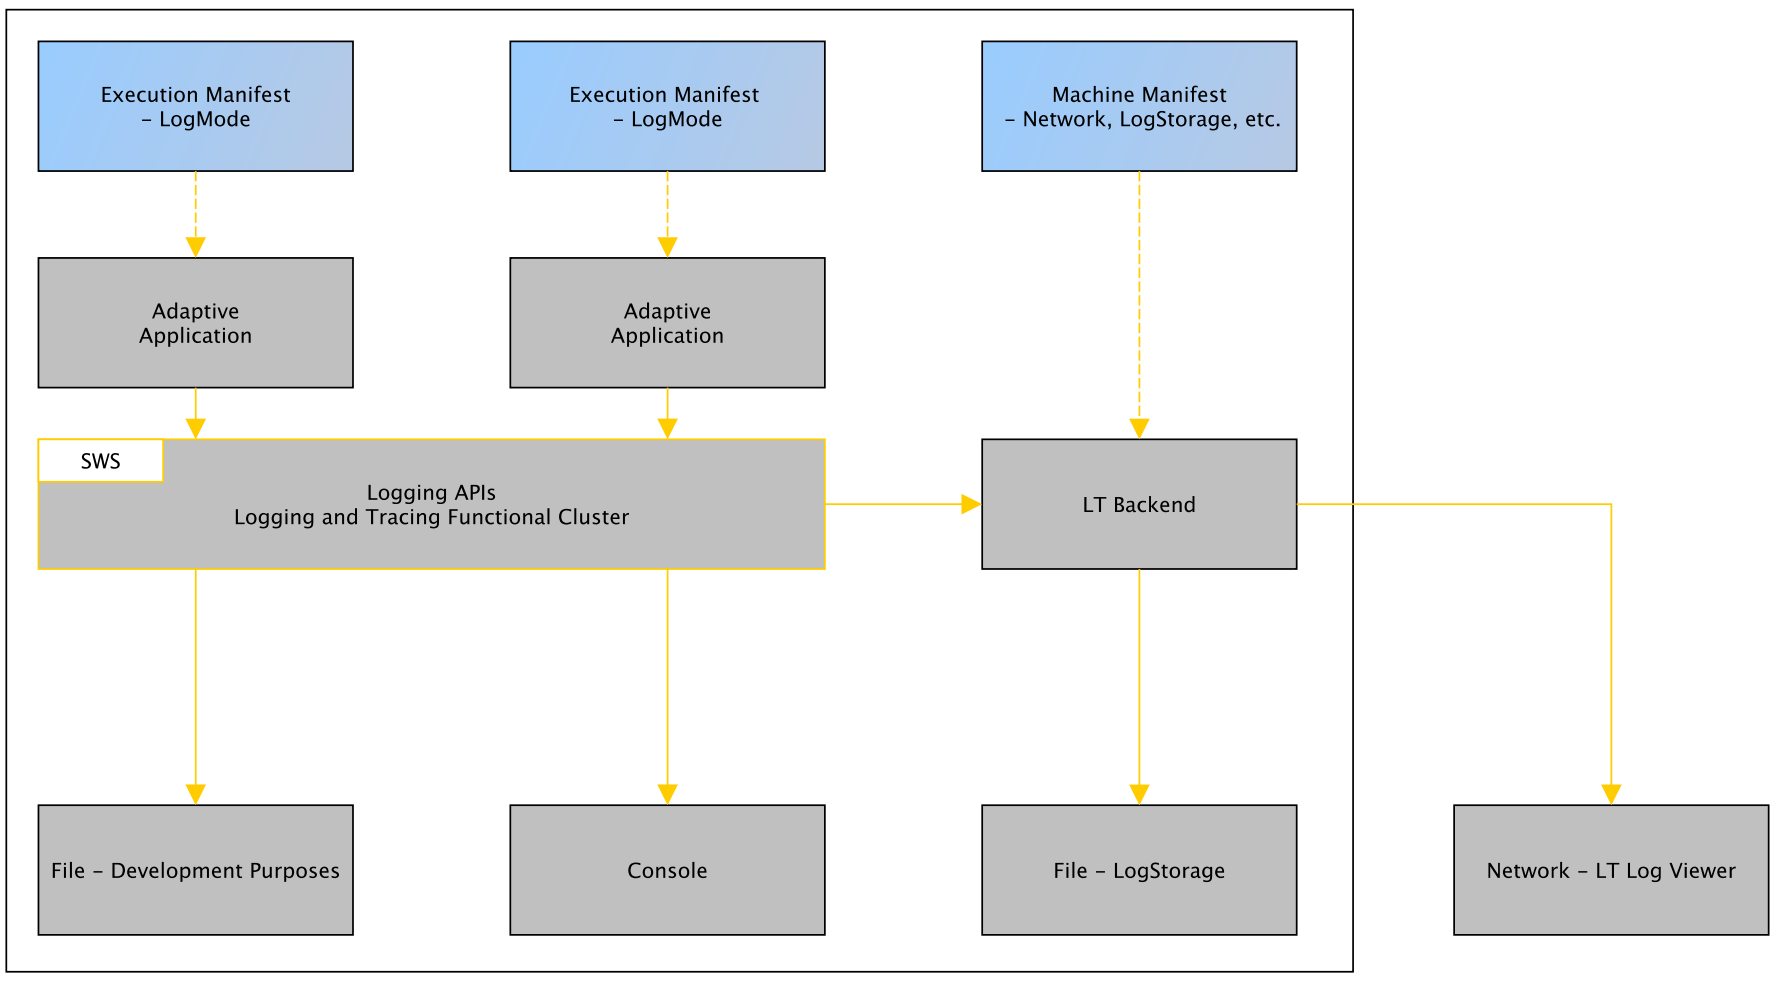
\includegraphics[width=1\textwidth]{Images/chapter2/log_mode.png}
%     \vspace{0.5cm}
%     \caption{Log Mode \cite{autosar_log_trace}}
%     \label{fig:log_mode}
% \end{figure}

% \subsubsection{Logging Contexts and Application IDs:}

% To effectively manage and distinguish logging data across a distributed system, the AUTOSAR Adaptive Platform utilizes a hierarchical identification scheme consisting of Application IDs and Logging Contexts.

% \paragraph*{Application IDs:}
% To distinguish the logs of different application instances within a system, every Application process must be assigned a specific Application ID. This identifier serves as a string value that associates generated logging information with its specific originating user application. While uniqueness across different ECUs is not required (as the ECU ID acts as a differentiator), the system integrator bears the responsibility of ensuring that each Application process instance within a single ECU possesses a unique Application ID. This configuration is typically supplied through the application execution manifest, which allows integrators to perform consistency checks. Because the Application ID string might be short or cryptic due to implementation limits, an optional Application Description can be provided as descriptive text to further identify the application instance.

% \paragraph*{Logging Contexts:}
% To allow for finer granularity within a single Application process, the platform uses Logging Contexts to distinguish logs from different logical groups or internal functional units. Each context is defined by a Context ID, which is a string identifier that must be unique within the scope of that specific Application process. Unlike the Application ID, the Context ID is assigned by the developer and is not modeled in the manifest. This structure is particularly important for software libraries running within an application's scope; they should reserve their own Context IDs to differentiate their internal logs from those of the parent application or other libraries. Similar to the application level, a Context Description string must be provided to offer a human-readable explanation of the context.

% \paragraph*{Initialization and Usage:}
% The connection between these identifiers is established when the application initializes the logging framework. An application process creates a logger instance for a specific context by calling the \texttt{ara::log::CreateLogger} function, passing the specific Context ID, Context Description, and optionally a default log level. This function creates a logger context instance internally within the Logging framework and returns a reference to the application, ensuring the context is registered against the back-end. Consequently, all log messages generated through this logger instance are tagged with both the Application ID (derived from the manifest) and the specific Context ID, allowing for precise filtering and analysis.

% \paragraph*{Architecture Overview:}
% The Figure \ref{fig:log_arch} above illustrates the high-level architecture where these logging contexts operate, showing the interaction between the Adaptive Application and the Logging Functional Cluster


\subsection{Log and Trace (\texttt{ara::log})}

The Log and Trace functional cluster (\texttt{ara::log}) provides a standardized C++ interface for Adaptive Applications to forward diagnostic and trace information to various output destinations (sinks). It is designed to maintain platform stability by managing system resources and buffering data during high-load scenarios. To efficiently organize the vast amount of vehicle data, \texttt{ara::log} employs a strict hierarchical identification system and severity-based filtering mechanisms.

\begin{figure}[h]
    \centering
    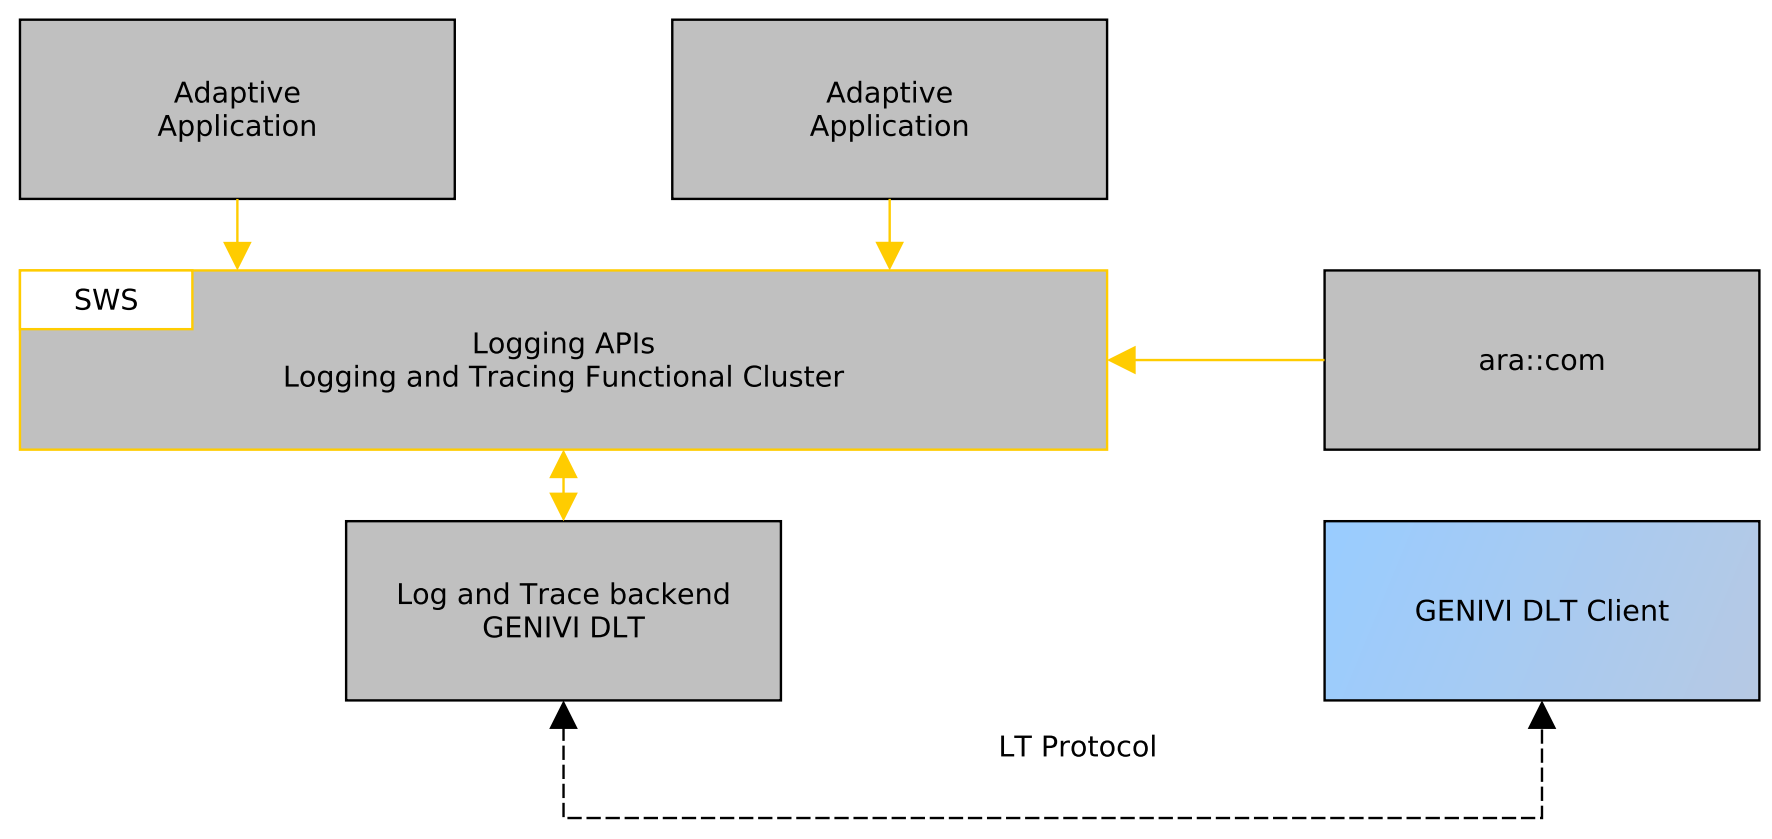
\includegraphics[width=0.9\textwidth]{Images/chapter2/log_arch.png}
    \vspace{0.5cm}
    \caption{Log and Trace Overview \cite{autosar_log_trace}}
    \label{fig:log_arch}
\end{figure}

\subsubsection{Severity Levels and Filtering}
To prevent resource exhaustion, \texttt{ara::log} categorizes messages using predefined severity levels, ranging from \texttt{kFatal} (0x01) and \texttt{kError} (0x02) to \texttt{kDebug} (0x05) and \texttt{kVerbose} (0x06). Applications are configured with a specific severity threshold; the framework only processes and transmits messages that meet or exceed this limit. This dynamic filtering ensures that excessive debug information is discarded during normal production operation, thereby conserving CPU and network bandwidth. Developers can easily generate logs using dedicated API methods such as \texttt{LogInfo()} or \texttt{LogError()}, which return a pre-configured \texttt{LogStream} object.

\subsubsection{Log Sinks and Output Bindings}
The framework decouples the logging API from the physical data destinations, known as Log Sinks. The routing behavior is configured within the Machine Manifest via the \texttt{DltLogSink} meta-class. The primary output bindings include:
\begin{itemize}
    \item \textbf{Console Binding:} Directs formatted messages to the standard console output, utilizing specific rules for separating arguments and rendering raw data.
    \item \textbf{File Binding:} Stores logs persistently on non-volatile storage, primarily utilized for development and integration testing.
    \item \textbf{Network (DLT) Binding:} Forwards messages over an Ethernet bus to a remote client (e.g., a DLT Viewer) using the standardized Log and Trace (LT) protocol. This mode supports bandwidth monitoring and maps C++ data types to specific DLT payloads.
\end{itemize}

\begin{figure}[h]
    \centering
    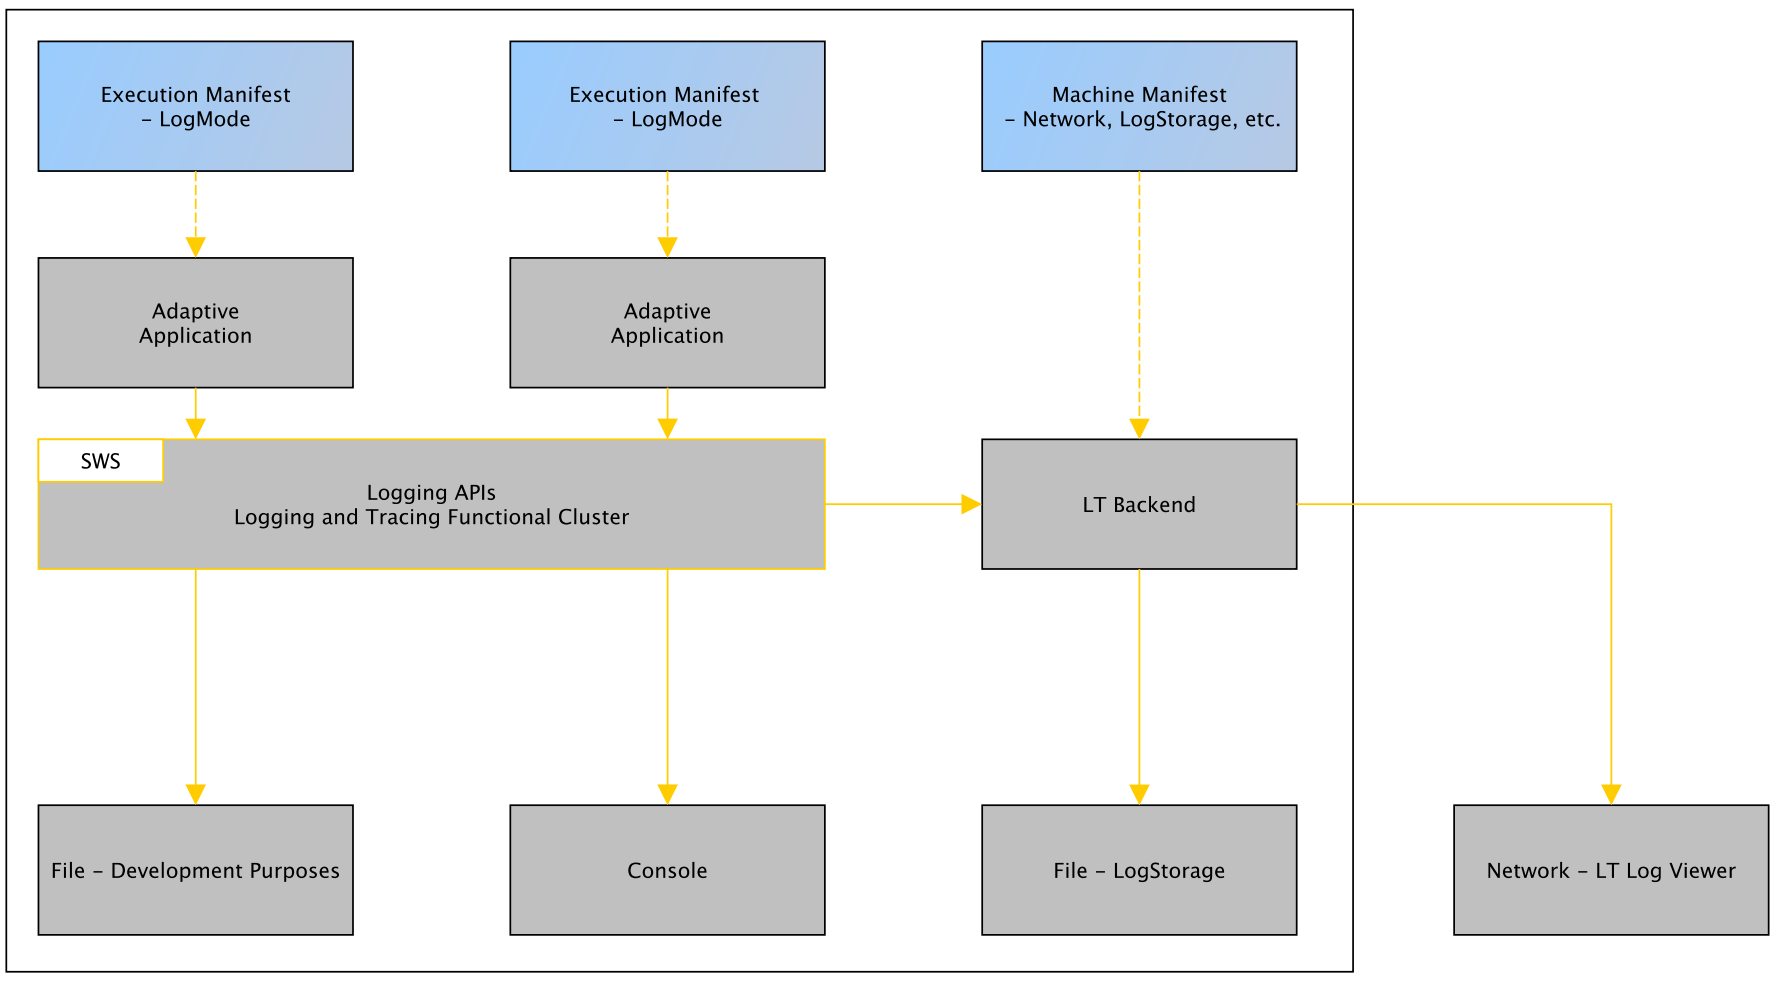
\includegraphics[width=0.9\textwidth]{Images/chapter2/log_mode.png}
    \vspace{0.5cm}
    \caption{Log Mode Configuration \cite{autosar_log_trace}}
    \label{fig:log_mode}
\end{figure}

\subsubsection{Application and Context Identification}
To track the origin of log messages across a distributed system, \texttt{ara::log} assigns a unique {Application ID} to every process instance, typically defined in the execution manifest. For finer granularity, developers define {Context IDs} to distinguish logs from different logical functional units or libraries within the same application. When an application calls \texttt{ara::log::CreateLogger}, it binds the specific Context ID to the logger instance. Consequently, all generated messages are tagged with both the Application ID and Context ID, enabling precise sorting and fault tracing on the backend.

\section{Development Toolchains}
PopcornSAR is a specialized Software-Defined Vehicle (SDV) tool and platform vendor focusing on the AUTOSAR Adaptive Platform to support automotive projects through advanced tools and engineering services. Their core design tool, {AutoSAR.io}, serves as a comprehensive authoring environment for modeling and configuring both Adaptive and Classic AUTOSAR platforms, offering features like graphical modeling, code generation, and interoperability with formats such as CAN DBC and COVESA VSS. This is complemented by {PARA}, an independently developed software framework designed for High-Performance Computing (HPC) that provides essential Adaptive AUTOSAR Functional Clusters---including communication (\texttt{ara::com}), execution management (\texttt{ara::exec}), and functional safety (\texttt{ara::phm})---to enable flexible and secure vehicle system development.

\begin{figure}[h]
    \centering
    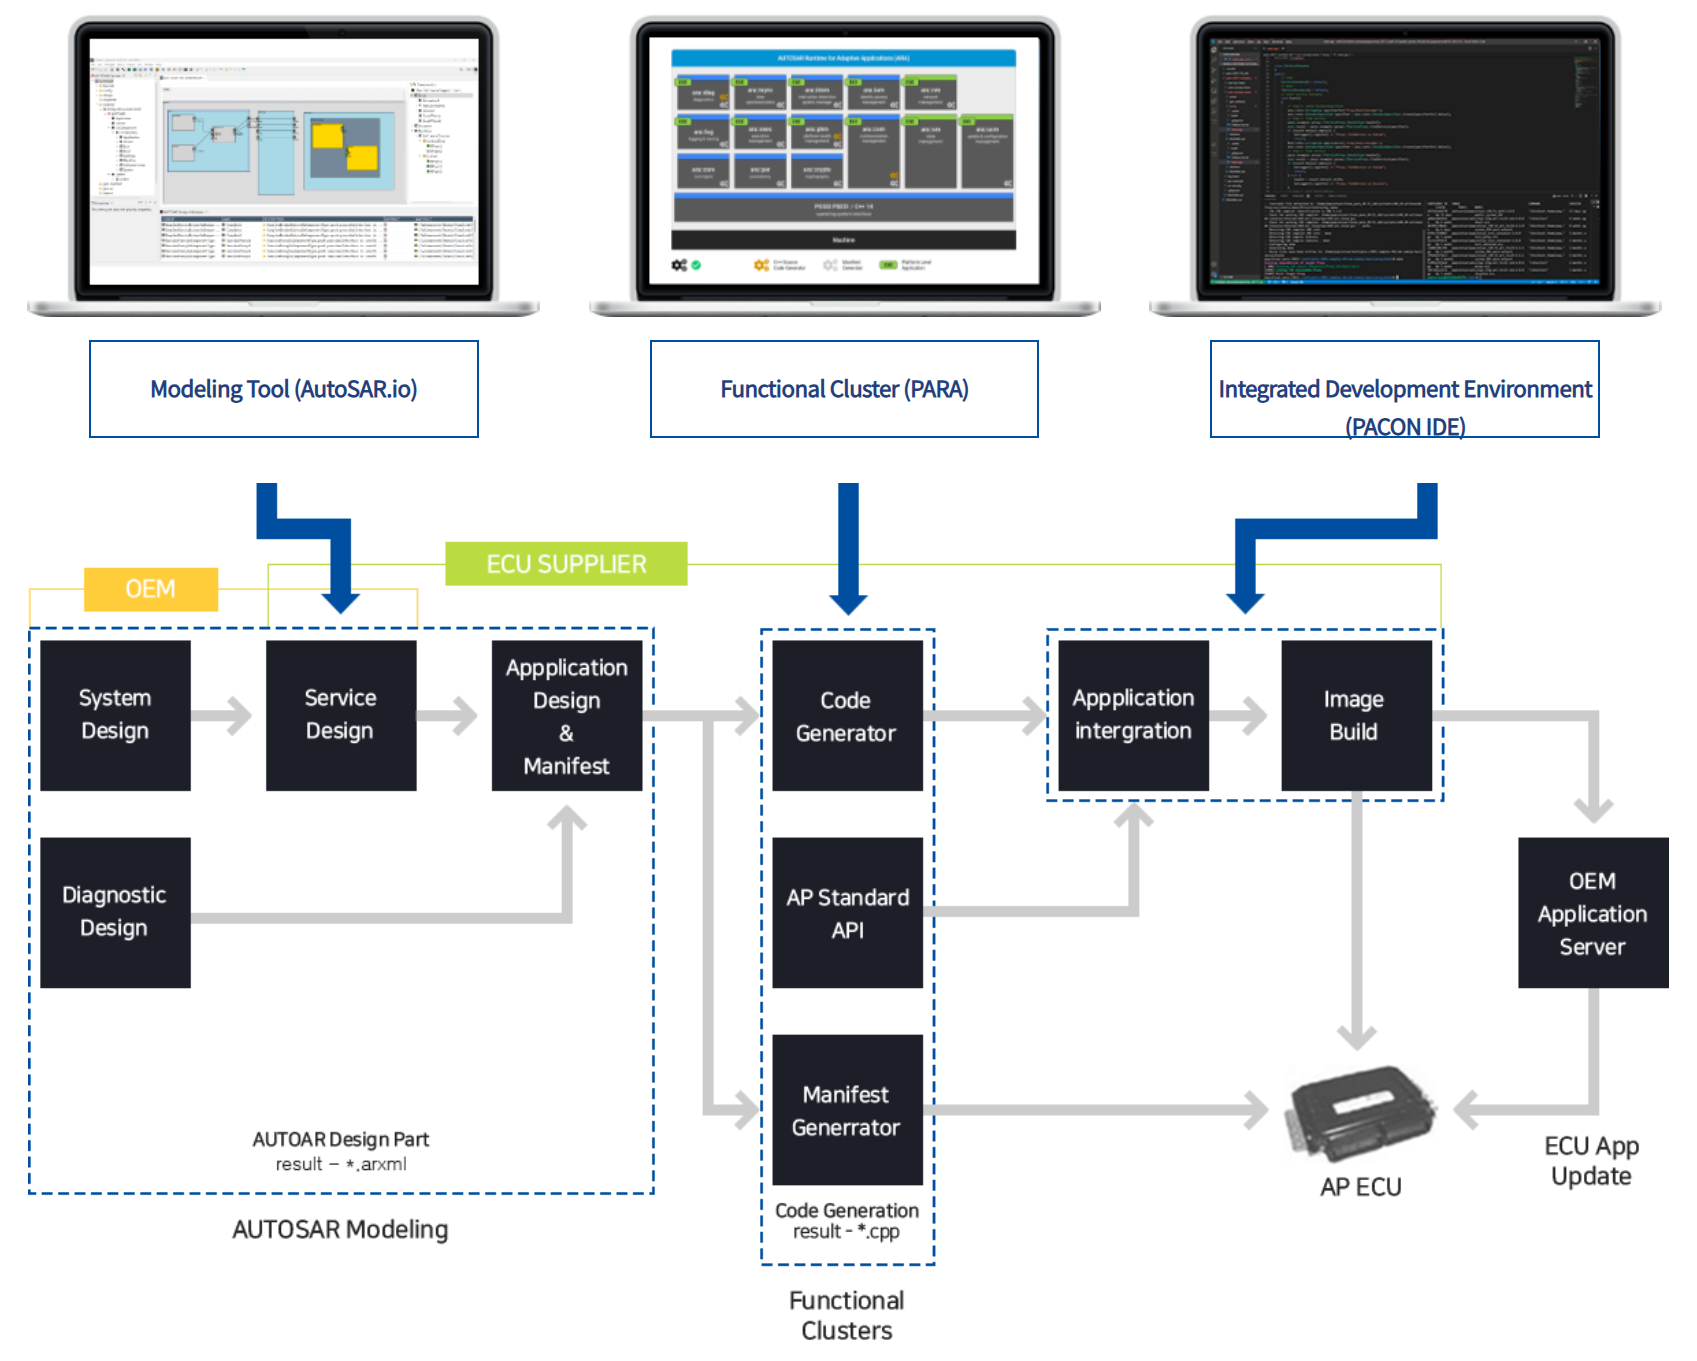
\includegraphics[width=1\textwidth]{Images/chapter2/tool_breakdowntool.png}
    \vspace{0.5cm}
    \caption{PopcornSAR Toolchain Breakdown \cite{popcornsar_intro}}
    \label{fig:popcornsar_toolchain}
\end{figure}

\subsection{AutoSAR.io}

AutoSAR.io is a powerful authoring tool developed by PopcornSAR, designed for the modeling and configuration of AUTOSAR projects within automotive systems. It serves as a comprehensive, future-proof development environment that supports the entire engineering spectrum, including System Architecture as well as both the Adaptive and Classic AUTOSAR Platforms. The tool is specifically built to empower customers in the efficient development of Software-Defined Vehicles (SDV), enabling them to significantly reduce complexity and accelerate the advancement of future automotive architectures.

Key features of AutoSAR.io include the capability to handle AUTOSAR System Design and the implementation of both Adaptive and Classic Platforms within a single tool. It streamlines the engineering process through graphical modeling for software components, internal behavior, and in-vehicle networks, complemented by a spreadsheet-style configurator and full support for the AUTOSAR methodology. The platform includes specialized designers for elements such as Adaptive Applications, Machines, Data Types, and Interfaces, along with ECU configuration for realtime environment (RTE), OS, and basic software (BSW). Additionally, AutoSAR.io functions as a robust code generator for AUTOSAR-compliant code and manifest files, and it offers seamless format conversion to integrate data models like CAN DBC, COVESA VSS, and existing ARXML into the AUTOSAR ecosystem.

\begin{figure}[h]
    \centering
    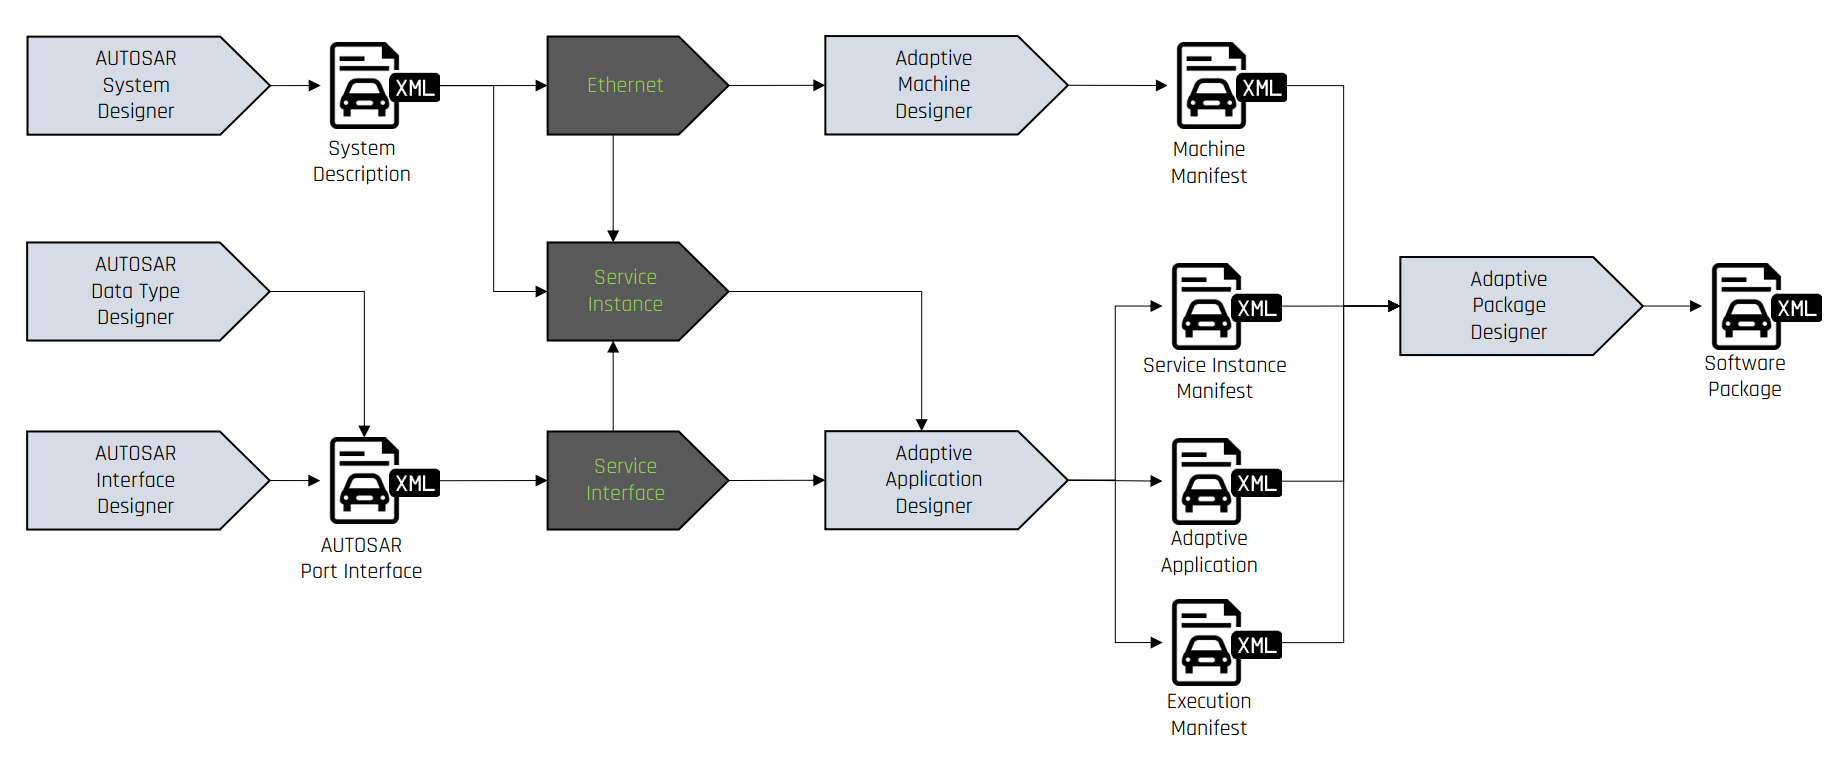
\includegraphics[width=1\textwidth]{Images/chapter2/aio_ap.png}
    \vspace{0.5cm}
    \caption{Adaptive Platform Workflow in AutoSAR.io \cite{popcornsar_intro}}
    \label{fig:autosar_io_ap}
\end{figure}


\begin{figure}[h]
    \centering
    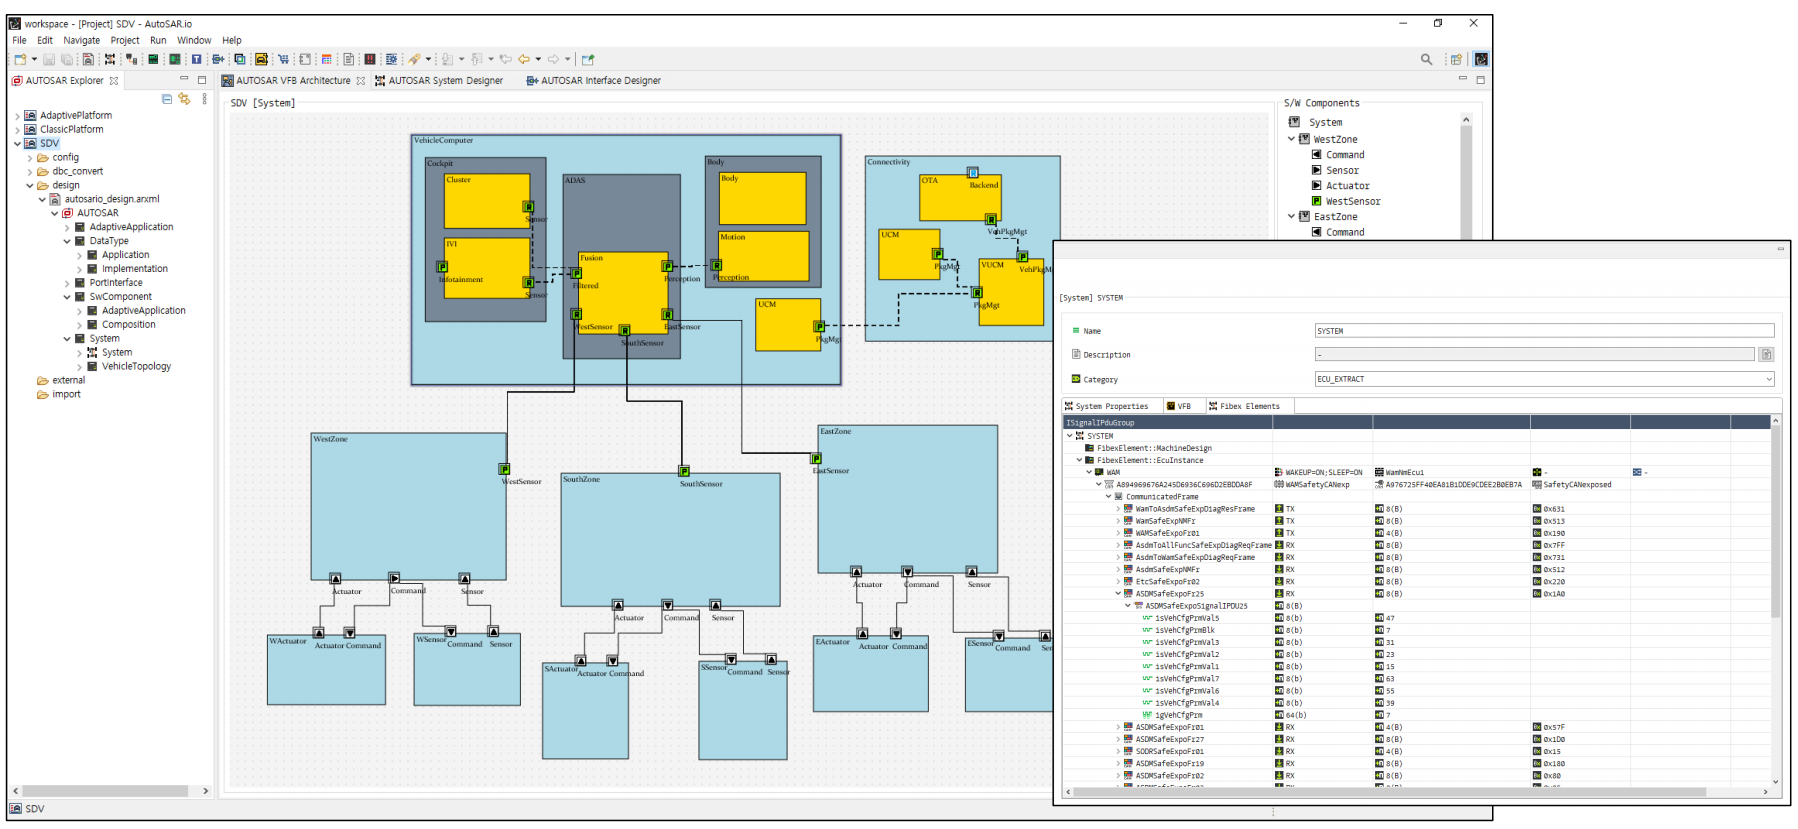
\includegraphics[width=1\textwidth]{Images/chapter2/aio_systemdesign.png}
    \vspace{0.5cm}
    \caption{AUTOSAR System Design in AutoSAR.io \cite{popcornsar_intro}}
    \label{fig:autosar_io_systemdesign}
\end{figure}

\begin{figure}[h]
    \centering
    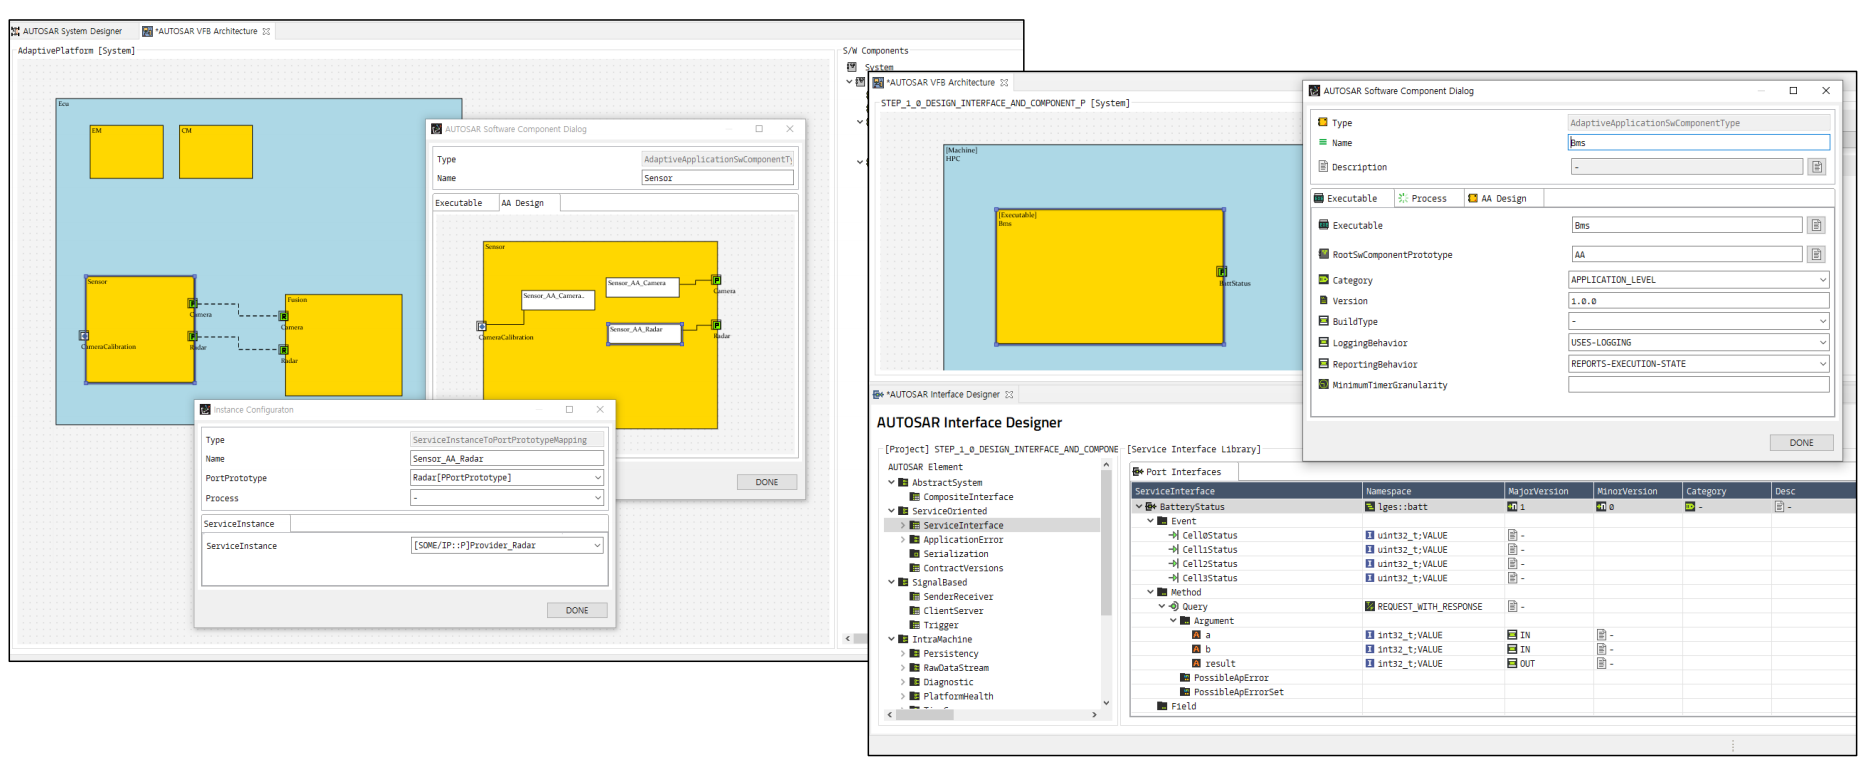
\includegraphics[width=1\textwidth]{Images/chapter2/aio_appldesign.png}
    \vspace{0.5cm}
    \caption{Application Design in AutoSAR.io \cite{popcornsar_intro}}
    \label{fig:autosar_io_appldesign}
\end{figure}


% \begin{figure}[h]
%     \centering
%     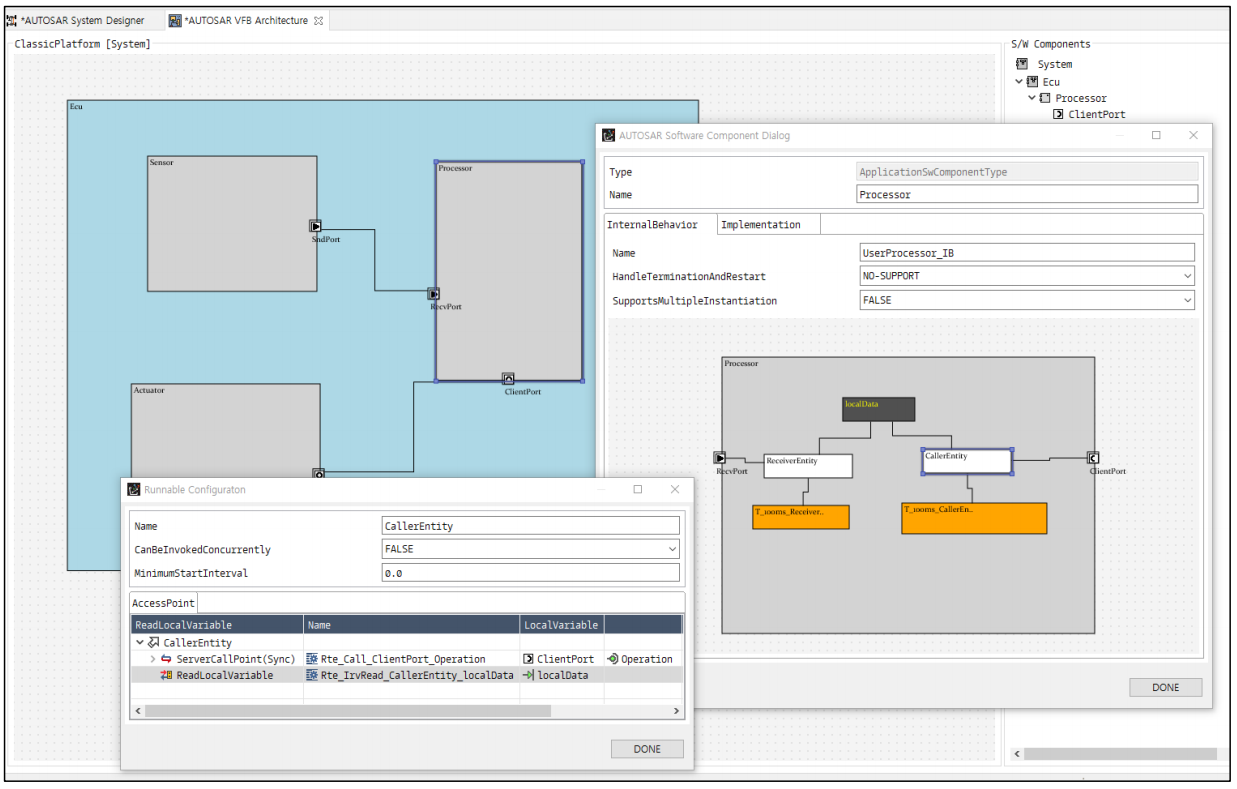
\includegraphics[width=1\textwidth]{Images/chapter2/aio_swdesign.png}
%     \vspace{0.5cm}
%     \caption{Software Component Design in AutoSAR.io \cite{popcornsar_intro}}
%     \label{fig:autosar_io_swdesign}
% \end{figure}

% \begin{figure}[h]
%     \centering
%     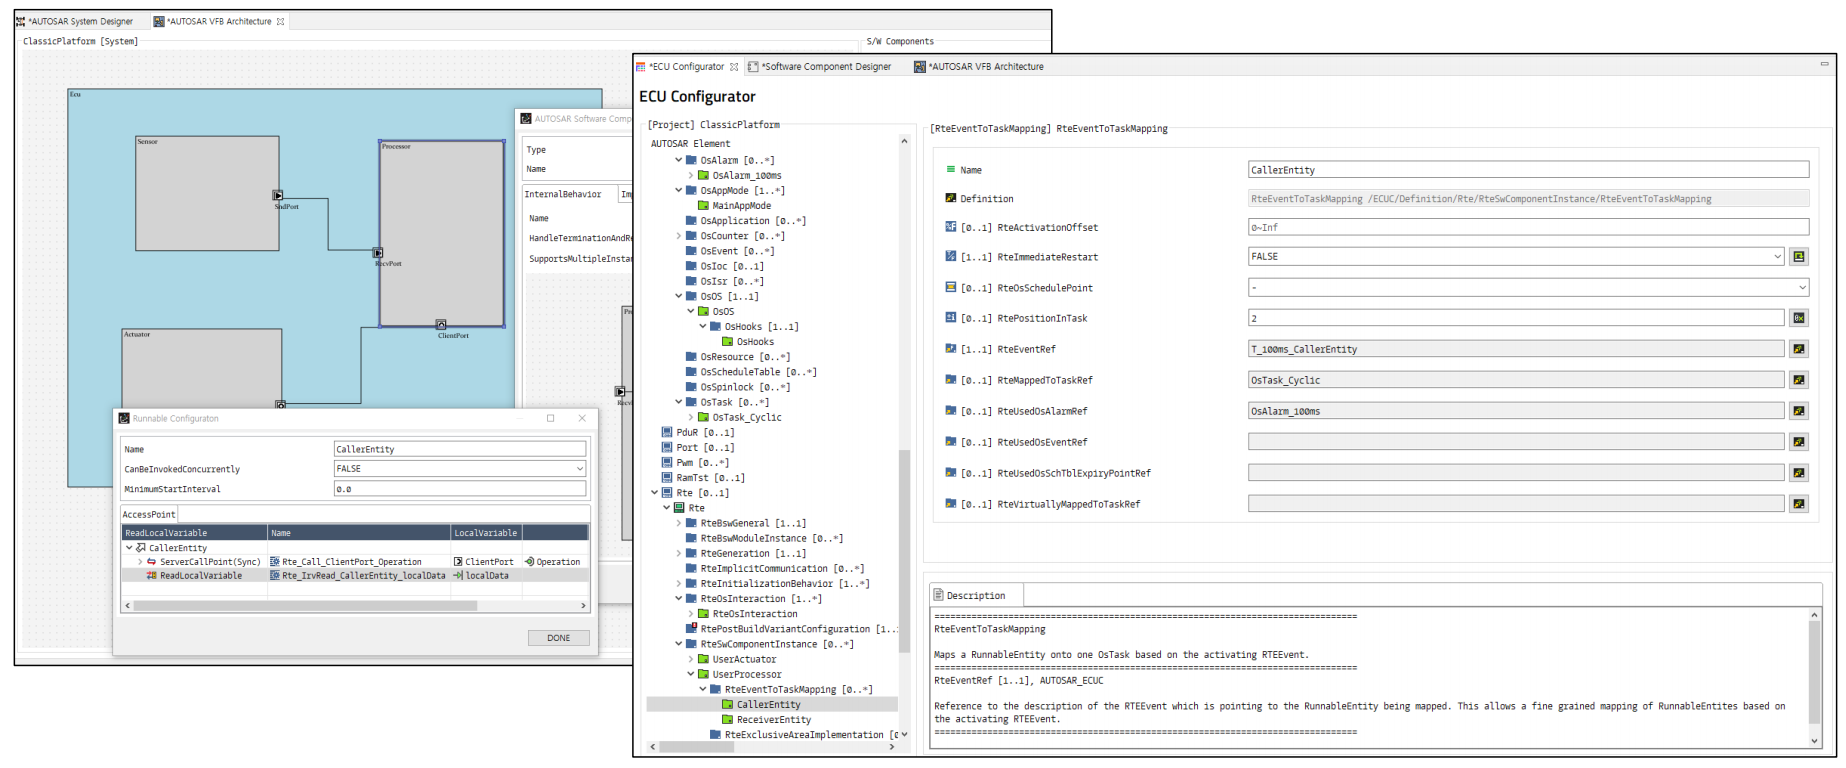
\includegraphics[width=1\textwidth]{Images/chapter2/aio_ecucfg.png}
%     \vspace{0.5cm}
%     \caption{ECU Configuration in AutoSAR.io \cite{popcornsar_intro}}
%     \label{fig:autosar_io_ecucfg}
% \end{figure}

AutoSAR.io is a powerful modeling tool that supports Code Generator of AUTOSAR-compliant code and manifest files. It streamlines development workflows while enabling full customization based on customer-specific requirements.

\begin{figure}[h]
    \centering
    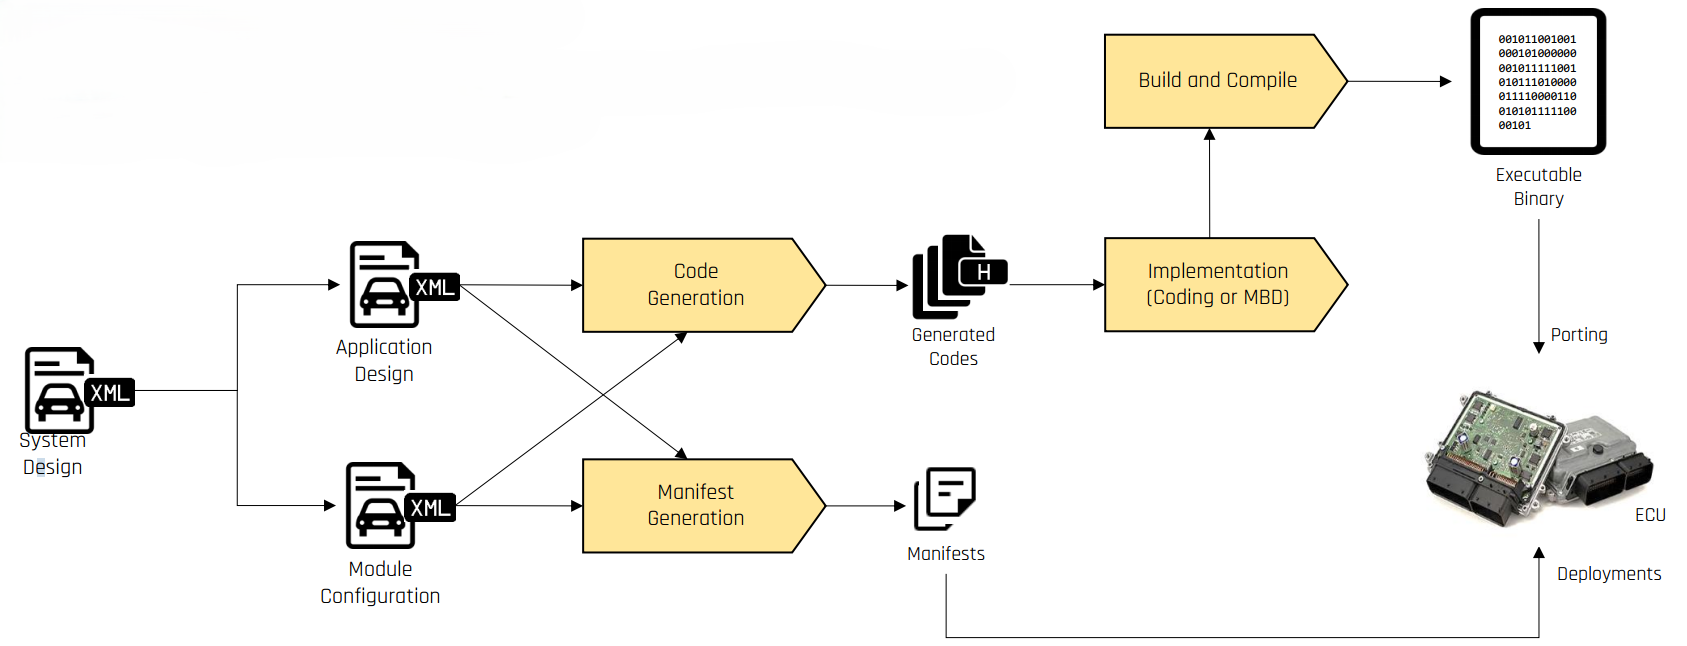
\includegraphics[width=1\textwidth]{Images/chapter2/aio_gen.png}
    \vspace{0.5cm}
    \caption{Code Generator Workflow in AutoSAR.io \cite{popcornsar_intro}}
    \label{fig:autosar_io_codegen}
\end{figure}

% AutoSAR.io supports seamless conversion of various data model formats such as CAN DBC, COVESA VSS, and AUTOSAR ARXML into AUTOSAR-compliant models. This allows smooth integration of existing vehicle data assets into the AUTOSAR eco-system.

% \begin{figure}[h]
%     \centering
%     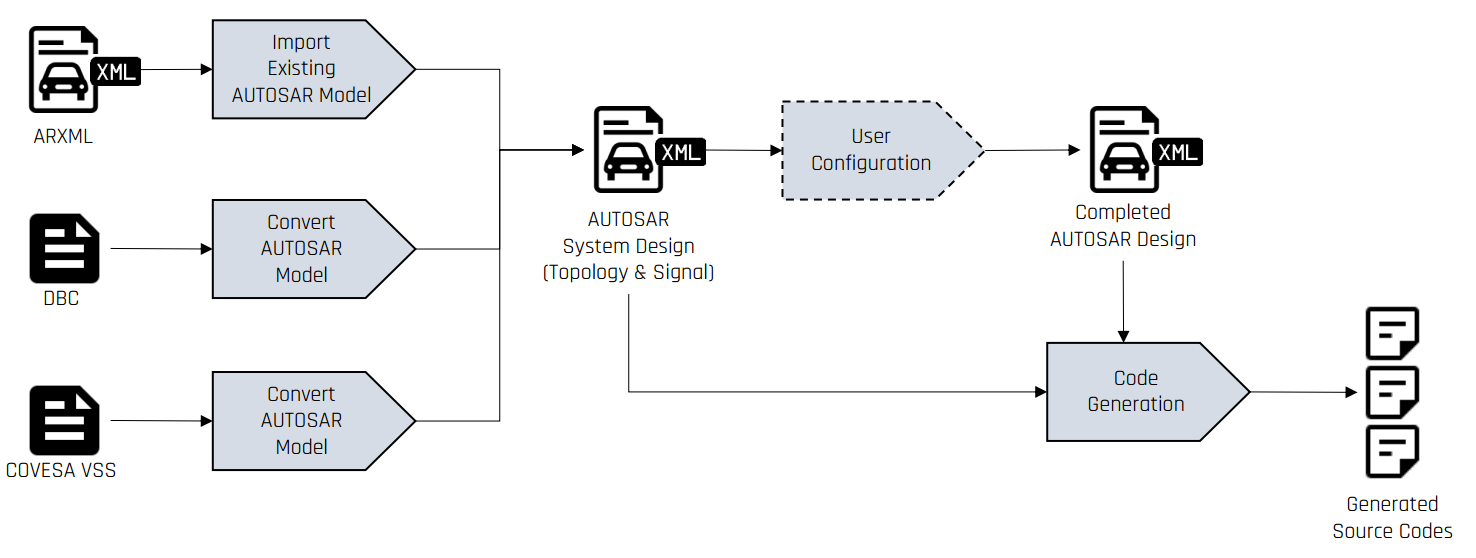
\includegraphics[width=1\textwidth]{Images/chapter2/aio_othergen.png}
%     \vspace{0.5cm}
%     \caption{Other Data Format Conversion Workflow in AutoSAR.io \cite{popcornsar_intro}}
%     \label{fig:autosar_io_othergen}
% \end{figure}
\newpage
\subsection{PARA}

PARA is PopcornSAR's ASIL-B certified AUTOSAR Adaptive Platform software framework, explicitly engineered for automotive HPC to accelerate the development of SDV. It delivers a comprehensive SOA that seamlessly integrates traditional automotive functions with modern IT frameworks like ROS2 and AI. To ensure robust operation across critical ADAS and VCU applications, PARA provides a suite of specialized functional clusters: \texttt{ara::com} manages diverse communication protocols (SOME/IP, DDS, zero-copy IPC, and Signal-To-Service), \texttt{ara::exec} orchestrates safe application lifecycles, and \texttt{ara::phm} enforces ISO 26262-compliant health monitoring. Furthermore, the SDK incorporates rigorous security mechanisms (\texttt{ara::idsm}, \texttt{ara::crypto}), diagnostic capabilities (\texttt{ara::diag}), secure Over-The-Air updates (\texttt{ara::ucm}), and legacy signal-based bridging (\texttt{para::sigcom}, \texttt{ara::aag}) to form a highly scalable, secure, and future-proof automotive development ecosystem.


\begin{figure}[h]
    \centering
    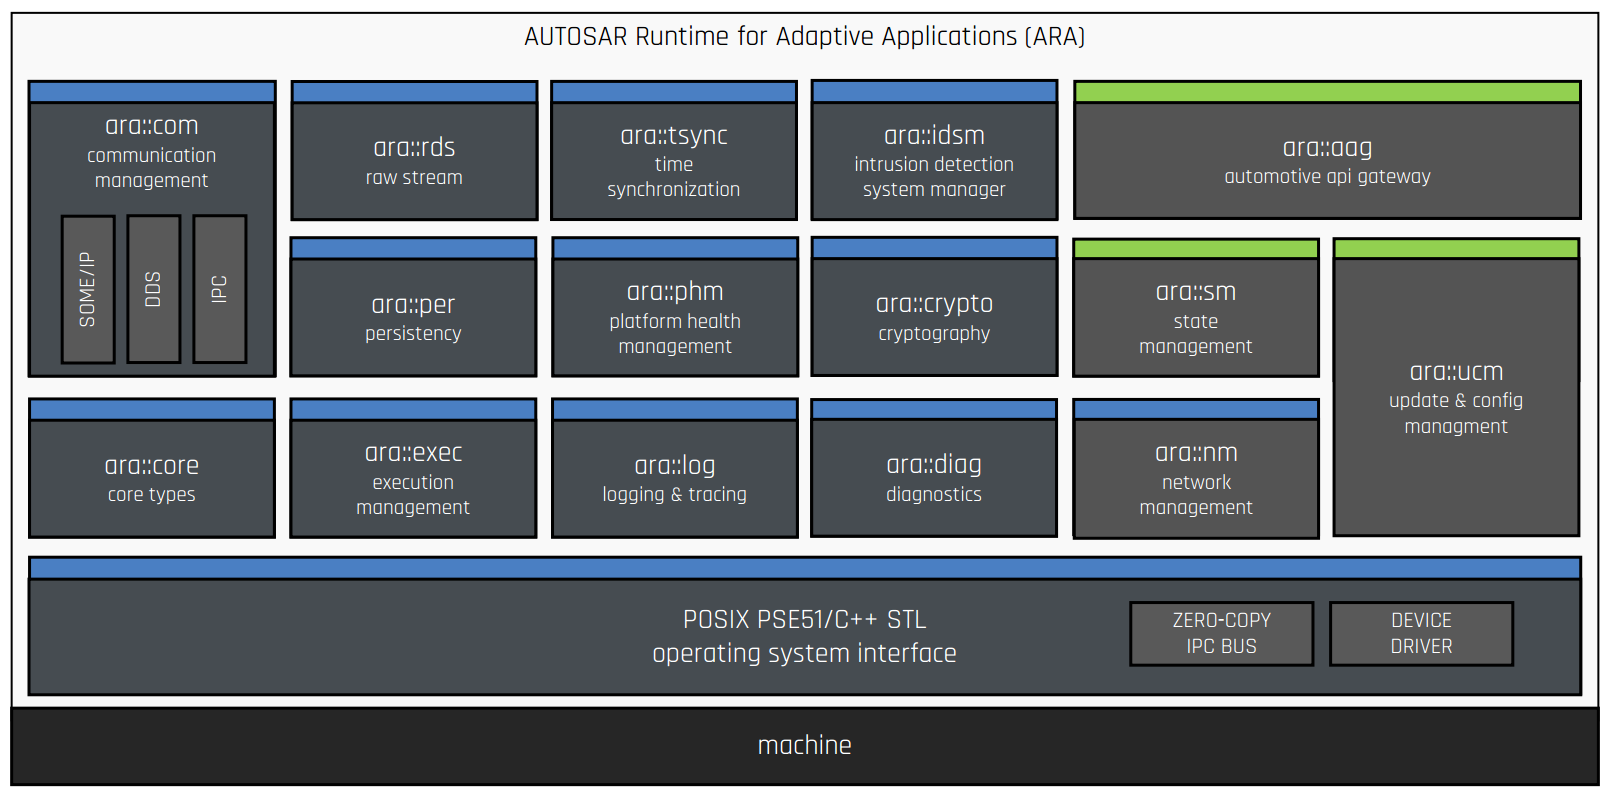
\includegraphics[width=1\textwidth]{Images/chapter2/para_basemodule.png}
    \vspace{0.5cm}
    \caption{Base Modules in PARA \cite{popcornsar_intro}}
    \label{fig:para_basemodule}
\end{figure}
\newpage
\paragraph*{Communication}(\texttt{ara::com})

\begin{figure}[h]
    \centering
    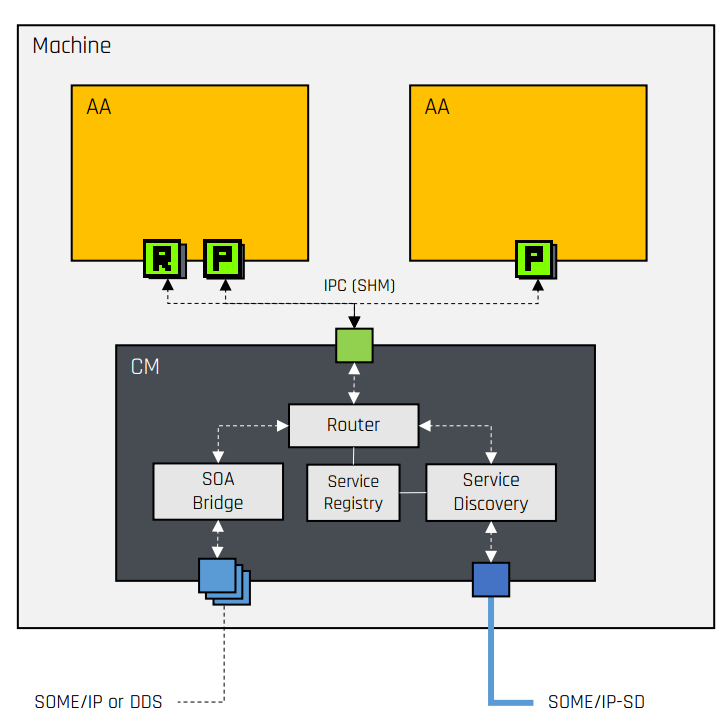
\includegraphics[width=0.5\textwidth]{Images/chapter2/para_com.png}
    \vspace{0.5cm}
    \caption{Communication in PARA \cite{popcornsar_intro}}
    \label{fig:para_com}
\end{figure}

PARA provides the complete product level for Service-Oriented Communication features. With PARA, \texttt{ara::com} provides full API and management for implementing service instances with application.

Some Protocols for SOA are supported in PARA like SOME/IP, DDS, and IPC (For Intra-machine).

PARA has base scheme for High-Performance IPC with zero-copy. 


\paragraph*{Execution Management}(\texttt{ara::exec})


\begin{figure}[h]
    \centering
    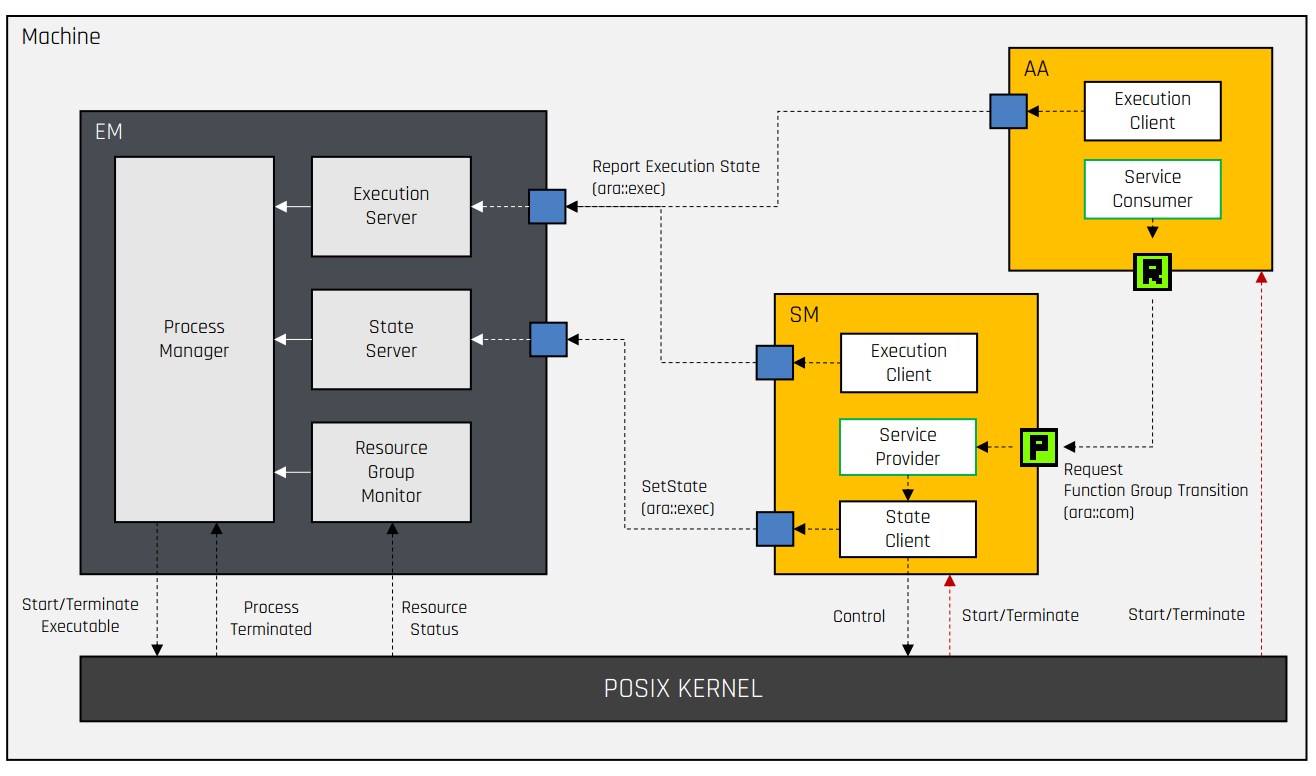
\includegraphics[width=0.8\textwidth]{Images/chapter2/para_exec.png}
    \vspace{0.5cm}
    \caption{Execution Management in PARA \cite{popcornsar_intro}}
    \label{fig:para_exec}
\end{figure}

With PARA, ara::exec provides management of applications with your configured scenario with state, execution dependency and resource statues. It also supports safe starting and termination of applications and machine.

After introducing the toolchain used to configure and generate Adaptive AUTOSAR applications, the following sections describe the AI models and inference runtime that provide the perception capability of the prototype.
% \newpage

% \section{YOLO (You Only Live Once) Model and MobileNetV4}



% \subsection{Overview of YOLO}

% The landscape of computer vision, particularly within the high-stakes domain of autonomous driving and Advanced Driver Assistance Systems (ADAS), has been irrevocably altered by the advent and evolution of the \textbf{``You Only Look Once"} (\textbf{YOLO}) architecture. As vehicles move towards higher levels of autonomy, the requirement for perception systems shifts from merely accurate classification to a rigorous demand for low-latency, high-frequency spatial understanding. Traffic light detection represents a particularly unforgiving subset of this domain: the targets are small, state-variant, and environmentally volatile, yet the system’s failure tolerance is effectively zero. This section explores the theoretical underpinnings of YOLO, tracing its dominance over two-stage detectors, and analyzes its suitability for the specific constraints of real-time traffic signal recognition.

% \subsubsection{The Single-Stage Revolution}

% Prior to the introduction of YOLO in 2015, the state-of-the-art in object detection was dominated by Region-based Convolutional Neural Networks (R-CNN) and its successors. These architectures operated on a "propose-and-verify" paradigm where a dedicated mechanism would hypothesize thousands of potential object locations before a classifier verified them. While this method achieved high average precision, it suffered from a fundamental decoupling of localization and classification, creating a computational bottleneck that rendered real-time performance on embedded hardware nearly impossible. YOLO proposed a radical unification by reframing object detection not as a classification task applied to generated regions, but as a single regression problem. In this paradigm, a single neural network processes the full image in one forward pass, predicting bounding box coordinates and class probabilities directly from the feature maps.

% This "single-shot" approach yields decisive advantages for traffic light detection. First, it enables global contextual reasoning. Unlike sliding window or region proposal approaches that see only a subset of the image pixels at any given time, the YOLO architecture views the entire image during both training and inference. This allows the network to implicitly encode contextual information about object classes, such as inferring the likelihood of a traffic light based on the presence of a pole or the geometry of an intersection, thereby significantly reducing background false positives. Second, YOLO offers inference latency stability. The processing time of a YOLO network is effectively constant for a given input resolution, regardless of the number of objects in the scene. For safety-critical control loops in autonomous vehicles, this deterministic latency is non-negotiable, ensuring the perception system delivers state estimates at a fixed cadence to the planning module.

% \subsubsection{Choosing YOLO26 for Real-Time Detection}
% The decision to utilize YOLO11 (released late 2024) for traffic light detection is driven by its specific architectural refinements designed for efficiency and small-object detection. YOLO11 represents a significant evolution over predecessors like v5 and v8, introducing enhanced feature aggregation through C3k2 blocks and C2PSA attention modules. These components significantly improve the extraction of fine-grained features necessary for resolving distant traffic lights. Furthermore, the YOLOv11n (Nano) variant achieves higher Mean Average Precision (mAP) than previous nano models with approximately 22\% fewer parameters. This parameter efficiency is critical for the constrained compute environments of embedded vehicular Electronic Control Units (ECUs), allowing for sophisticated detection logic without exceeding thermal or power budgets.


% \subsection{The YOLO Algorithmic Architecture}
% In this proposed system, while the MobileNetV4 backbone handles the heavy lifting of feature extraction, the detection logic relies on the advanced YOLOv11 Neck and Head. This architecture departs from previous iterations by introducing specific modules that optimize the feature fusion process and employs an anchor-free, decoupled head paradigm.

% \subsubsection{The Grid System and Feature Fusion (C3k2)}

% The core of YOLOv11's spatial reasoning remains its hierarchical grid system, derived from a Path Aggregation Network (PANet). The input image is not processed as a monolith but is partitioned into grids of varying granularity. The input image $I$ is processed into feature maps at three distinct scales: P3 (stride 8), P4 (stride 16), and P5 (stride 32). The Neck is responsible for fusing these maps to combine the semantic richness of deep layers with the spatial precision of shallow layers.

% A primary innovation in the YOLOv11 Neck is the use of the C3k2 (Cross Stage Partial with Kernel Size 2) block, which replaces the C2f block found in YOLOv8. The C3k2 block utilizes optimized kernel sizes and a streamlined gradient path, allowing for customizable kernel configurations. This design enables the model to extract features with faster processing speeds on hardware accelerators. For traffic light detection, this efficient fusion is critical when processing high-resolution images, such as $1280 \times 1280$ pixels, which are often required to resolve small signal lights. The C3k2 block prevents the feature fusion stage from becoming a latency bottleneck, ensuring the semantic context of the intersection is merged with the fine spatial detail of the signal head without incurring excessive computational cost.

% \subsubsection{C2PSA: Spatial Attention for Small Objects}

% A defining feature of YOLOv11 logic is the inclusion of the C2PSA (Cross Stage Partial with Spatial Attention) module, typically positioned at the end of the feature extraction phase. The C2PSA module introduces a parallel branch that computes a spatial attention map, forcing the network to weight specific pixels more heavily before passing features to the detection head. In the context of traffic lights, which often occupy less than 1\% of the total image area, background noise from the sky, buildings, or trees can dominate the feature map. The C2PSA mechanism effectively suppresses this background noise and amplifies the activation of the relevant signal pixels. This targeted attention significantly improves the recall for distant lights, ensuring that the network focuses its capacity on the objects of interest rather than the surrounding clutter.

% \subsubsection{Anchor-Free Bounding Box Regression}

% YOLOv11 employs a fully anchor-free detection head, a departure from older versions that relied on pre-defined anchor boxes. Instead of predicting offsets from prototypical shapes, YOLOv11 predicts the bounding box geometry directly from the center of the grid cell. For a grid cell at location $(c_x, c_y)$ that is deemed responsible for an object, the network regresses four values representing the distances to the box edges: Left ($l$), Top ($t$), Right ($r$), and Bottom ($b$). The predicted bounding box $\hat{B}$ is formulated as:

% \begin{equation}
%     \hat{B} = [c_x - l, c_y - t, c_x + r, c_y + b]
% \end{equation}

% This approach eliminates the need to tune anchor hyperparameters for specific datasets, making the model naturally adaptive to the varying aspect ratios of traffic signals, whether they are vertical stacks, horizontal arrays, or single-aspect beacons.

% \subsubsection{The Loss Function: Task Alignment and CIoU}

% The training of the YOLOv11 head is guided by a composite loss function that enforces strict alignment between the classification and localization tasks. Traditional detectors often predict a high class score even if the bounding box is inaccurate. To counter this, YOLOv11 utilizes Task Aligned Loss (TAL). TAL dynamically assigns labels based on the quality of the prediction, calculating an alignment metric $t$ as $t = s^\alpha \times u^\beta$, where $s$ is the predicted classification score and $u$ is the Intersection over Union (IoU) between the predicted box and the ground truth. This ensures that high confidence scores are only assigned to predictions that are both semantically correct and spatially precise.

% For localization, the system employs Complete IoU (CIoU) loss combined with Distribution Focal Loss (DFL). The CIoU loss minimizes geometric errors by considering overlap area, center point distance, and aspect ratio consistency. The formula is given by:

% \begin{equation}
%     \mathcal{L}_{CIoU} = 1 - IoU + \frac{\rho^2(b, b^{gt})}{c^2} + \alpha v
% \end{equation}


% Here, $\rho$ is the Euclidean distance between box centers, $c$ is the diagonal length of the smallest enclosing box, and $\alpha v$ measures the consistency of the aspect ratio. This forces the model to rapidly converge to the vertical rectangular shape typical of traffic lights. Furthermore, DFL handles the ambiguity of small, blurred traffic lights by modeling the box edges not as single deterministic numbers but as probability distributions. By optimizing the network to focus the probability density around the true edge location, DFL provides refined, sub-pixel accuracy that is vital for distant signals.

% \subsubsection{Post-Processing: Class-Agnostic NMS}

% Because the anchor-free head is dense, a single traffic light will often trigger detections in multiple adjacent grid cells. Non-Maximum Suppression (NMS) is the algorithm used to filter these duplicate candidates. For traffic light detection, Class-Agnostic NMS is strongly recommended. This logic prevents the physically impossible scenario of detecting both a "Green Light" and a "Red Light" in the exact same spatial location. By suppressing overlapping boxes regardless of their class label, the model is forced to commit to the single highest-confidence state, thereby reducing conflicting outputs for the downstream planning system.

% \subsection{MobileNetV4 Backbone Architecture}
% To maximize efficiency on edge hardware such as the Raspberry Pi or NVIDIA Jetson, this report proposes replacing the standard YOLO backbone with MobileNetV4 (MNv4). MNv4, introduced in 2024, represents the culmination of research into efficient neural network design, prioritizing "Universal Efficiency" to ensure operations run fast across CPUs, GPUs, and DSPs without the fragmentation seen in previous versions.
% \subsubsection{Evolution of MobileNets: From V1 to V4}

% The MobileNet lineage began with \textbf{MobileNetV1}, which introduced Depthwise Separable Convolutions to factorize standard convolution into spatial and channel steps, reducing computation by approximately nine times. \textbf{MobileNetV2} subsequently introduced the Inverted Residual Block and Linear Bottlenecks to preserve information flow in low-dimensional spaces. \textbf{MobileNetV3} later incorporated Neural Architecture Search (NAS) and Squeeze-and-Excitation (SE) blocks. However, V3's heterogeneous blocks and complex activation functions often resulted in poor performance on DSPs due to synchronization overhead. \textbf{MobileNetV4} addresses these issues by using unified blocks optimized for the hardware "Roofline Model", ensuring that the architecture stays at the optimal ridge point of operational intensity where every cycle of memory transfer is matched by maximum computation.

% \subsubsection{Universal Inverted Bottleneck (UIB)}

% The core innovation of MobileNetV4 is the Universal Inverted Bottleneck (UIB). This is a flexible search block that unifies previous architectures by introducing two optional depthwise convolutions that can be enabled or disabled via NAS. The UIB can instantiate as a standard Inverted Bottleneck for capacity, a ConvNext block for cheaper spatial mixing, or a novel ExtraDW block. The ExtraDW variant is particularly beneficial for traffic light detection. By adding extra depthwise layers at a low computational cost, it significantly increases the network's receptive field. This allows the backbone to "see" the entire intersection context—such as the traffic pole arm or the road geometry—without the heavy computational penalty of large kernels, which is crucial for identifying signal heads amidst urban clutter.

% \subsubsection{Mobile Multi-Query Attention (MQA)}

% Standard Multi-Head Self-Attention (MHSA) is typically memory-bound on mobile chips, making it slow to execute. To overcome this, MNv4 introduces Mobile MQA (Multi-Query Attention). In this mechanism, all query heads share a single Key and Value head, and a spatial reduction is applied via a stride-2 depthwise convolution. The attention computation can be approximated as:

% \begin{equation}
%     \text{Attention}(Q, K, V) = \text{Softmax}\left(\frac{Q \cdot (SR(K))^T}{\sqrt{d_k}}\right) \cdot SR(V)
% \end{equation}

% This design provides a substantial speedup—approximately 39\% on EdgeTPUs—while retaining the global context capabilities of transformers. This global attention helps the model distinguish true traffic lights from reflections or neon signs by analyzing the broader scene context, a capability that pure CNNs often lack.

% \subsubsection{Integrating MobileNetv4 into YOLO}

% Integrating MobileNetV4 as the feature extractor for YOLOv11 creates a hybrid "YOLO-MNv4" architecture that is theoretically optimal for autonomous driving. On mobile accelerators like the Pixel EdgeTPU, MNv4 is approximately twice as fast as MobileNetV3 for equivalent accuracy due to its high operational intensity. Replacing the standard YOLOv11 backbone with MNv4 significantly reduces the floating-point operations (FLOPs) required per inference. This architecture specifically excels in occlusion handling, where the advanced receptive fields of the UIB blocks allow the model to infer the presence of a traffic light even when it is partially obscured by large vehicles, ensuring a robust and reliable perception system.
\section{YOLO (You Only Look Once) Model and MobileNetV4 Backbone}



\subsection{Overview of YOLO}

The landscape of computer vision, particularly within the high-stakes domain of autonomous driving and Advanced Driver Assistance Systems (ADAS), has been irrevocably altered by the advent and evolution of the {``You Only Look Once"} ({YOLO}) architecture. As vehicles move towards higher levels of autonomy, the requirement for perception systems shifts from merely accurate classification to a rigorous demand for low-latency, high-frequency spatial understanding. Traffic light detection represents a particularly unforgiving subset of this domain: the targets are small, state-variant, and environmentally volatile, yet the system’s failure tolerance is effectively zero. This section explores the theoretical underpinnings of YOLO, tracing its dominance over two-stage detectors, and analyzes its suitability for the specific constraints of real-time traffic signal recognition.

\subsubsection{The Single-Stage Revolution}

Prior to the introduction of YOLO in 2015, the state-of-the-art in object detection was dominated by Region-based Convolutional Neural Networks (R-CNN) and its successors. These architectures operated on a "propose-and-verify" paradigm where a dedicated mechanism would hypothesize thousands of potential object locations before a classifier verified them. While this method achieved high average precision, it suffered from a fundamental decoupling of localization and classification, creating a computational bottleneck that rendered real-time performance on embedded hardware nearly impossible. YOLO proposed a radical unification by reframing object detection not as a classification task applied to generated regions, but as a single regression problem. In this paradigm, a single neural network processes the full image in one forward pass, predicting bounding box coordinates and class probabilities directly from the feature maps.

This "single-shot" approach yields decisive advantages for traffic light detection. First, it enables global contextual reasoning. Unlike sliding window or region proposal approaches that see only a subset of the image pixels at any given time, the YOLO architecture views the entire image during both training and inference. This allows the network to implicitly encode contextual information about object classes, such as inferring the likelihood of a traffic light based on the presence of a pole or the geometry of an intersection, thereby significantly reducing background false positives. Second, YOLO offers inference latency stability. The processing time of a YOLO network is effectively constant for a given input resolution, regardless of the number of objects in the scene. For safety-critical control loops in autonomous vehicles, this deterministic latency is non-negotiable, ensuring the perception system delivers state estimates at a fixed cadence to the planning module.

\subsubsection{YOLO26 for Real-Time Detection}
The decision to utilize YOLO26 (released January 2026) for traffic light detection is driven by its specific architectural refinements designed for efficiency and small-object detection. YOLO26 represents a significant evolution over predecessors like YOLO11 and YOLOv8 \cite{yolo26}, introducing enhanced feature aggregation through C3k2 blocks, C2PSA attention modules, and a novel MuSGD optimizer. These components significantly improve the extraction of fine-grained features necessary for resolving distant traffic lights. Furthermore, YOLO26 removes the Distribution Focal Loss (DFL) module entirely, simplifying export and hardware compatibility, and delivers up to 43\% faster CPU inference compared to its predecessors. This computational efficiency is critical for the constrained compute environments of embedded vehicular Electronic Control Units (ECUs), allowing for sophisticated detection logic without exceeding thermal or power budgets.


\subsection{The YOLO Algorithmic Architecture}
In this proposed system, while the MobileNetV4 backbone handles the heavy lifting of feature extraction, the detection logic relies on the advanced YOLO26 Neck and Head. This architecture departs from previous iterations by introducing specific modules that optimize the feature fusion process and employs an anchor-free, decoupled head paradigm.

\subsubsection{The Grid System and Feature Fusion (C3k2)}

The core of YOLO26's spatial reasoning remains its hierarchical grid system, derived from a Path Aggregation Network (PANet). The input image is not processed as a monolith but is partitioned into grids of varying granularity. In the standard YOLO26-p2 configuration, the backbone produces feature maps at four scales: P2 (stride 4), P3 (stride 8), P4 (stride 16), and P5 (stride 32). In the proposed system, the Neck fuses these maps to combine the semantic richness of deep layers with the spatial precision of shallow layers.

A primary innovation in the YOLO26 Neck is the use of the C3k2 (Cross Stage Partial with Kernel Size 2) block, inherited from YOLO11 and refined in YOLO26. The C3k2 block utilizes a cross-stage partial design with customizable kernel configurations and a streamlined gradient path. This design enables the model to extract features with faster processing speeds on hardware accelerators. For traffic light detection in this system, images are processed at $416 \times 416$ pixels—a resolution chosen to balance inference speed with the spatial detail required to resolve signal heads on edge hardware. The C3k2 block prevents the feature fusion stage from becoming a latency bottleneck, ensuring the semantic context of the intersection is merged with the fine spatial detail of the signal head without incurring excessive computational cost.

\subsubsection{C2PSA: Spatial Attention for Small Objects}

A defining feature of YOLO26 logic is the inclusion of the C2PSA (Cross Stage Partial with Spatial Attention) module, typically positioned at the end of the feature extraction phase. The C2PSA module introduces a parallel branch that computes a spatial attention map, forcing the network to weight specific pixels more heavily before passing features to the detection head. In the context of traffic lights, which often occupy less than 1\% of the total image area, background noise from the sky, buildings, or trees can dominate the feature map. The C2PSA mechanism effectively suppresses this background noise and amplifies the activation of the relevant signal pixels. This targeted attention significantly improves the recall for distant lights, ensuring that the network focuses its capacity on the objects of interest rather than the surrounding clutter.

% \subsubsection{Anchor-Free Bounding Box Regression}

% YOLO26 employs a fully anchor-free detection head, a departure from older versions that relied on pre-defined anchor boxes. Instead of predicting offsets from prototypical shapes, YOLO26 predicts the bounding box geometry directly from the center of the grid cell. For a grid cell at location $(c_x, c_y)$ that is deemed responsible for an object, the network regresses four values representing the distances to the box edges: Left ($l$), Top ($t$), Right ($r$), and Bottom ($b$). The predicted bounding box $\hat{B}$ is formulated as:

% \begin{equation}
%     \hat{B} = [c_x - l, c_y - t, c_x + r, c_y + b]
% \end{equation}

% This approach eliminates the need to tune anchor hyperparameters for specific datasets, making the model naturally adaptive to the varying aspect ratios of traffic signals, whether they are vertical stacks, horizontal arrays, or single-aspect beacons.

% \subsubsection{The Loss Function: Task Alignment and CIoU}

% The training of the YOLO26 head is guided by a composite loss function that enforces strict alignment between the classification and localization tasks. Traditional detectors often predict a high class score even if the bounding box is inaccurate. To counter this, YOLO26 utilizes a Spatial and Task-Aligned Label assignment (STAL), a component of ProgLoss. STAL dynamically assigns labels based on the quality of the prediction, calculating an alignment metric $t$ as $t = s^\alpha \times u^\beta$, where $s$ is the predicted classification score, $u$ is the Intersection over Union (IoU) between the predicted box and the ground truth, and $\alpha$, $\beta$ are balancing hyperparameters. This ensures that high confidence scores are only assigned to predictions that are both semantically correct and spatially precise.

% For localization, YOLO26 employs Complete IoU (CIoU) loss. A key distinction from its predecessors is that {YOLO26 removes Distribution Focal Loss (DFL) entirely}-this simplifies the model graph, broadens hardware compatibility, and reduces export complexity. The CIoU loss minimizes geometric errors by jointly considering overlap area, center-point distance, and aspect ratio consistency. The formula is given by:

% \begin{equation}
%     \mathcal{L}_{CIoU} = 1 - \text{IoU} + \frac{\rho^2(b, b^{gt})}{c^2} + \alpha v
% \end{equation}

% where $v = \frac{4}{\pi^2}\left(\arctan\frac{w^{gt}}{h^{gt}} - \arctan\frac{w}{h}\right)^2$ measures aspect ratio consistency, $\alpha = \frac{v}{(1-\text{IoU})+v}$ is a trade-off parameter, $\rho$ is the Euclidean distance between predicted box center $b$ and ground-truth center $b^{gt}$, and $c$ is the diagonal length of the smallest enclosing box. This formulation forces the model to converge to the vertical rectangular shape typical of traffic light signal heads.

\subsubsection{Dual-Head Architecture and NMS-Free Inference}

YOLO26 features a dual-head architecture that provides flexibility for different deployment scenarios \cite{yolo26}:
\begin{itemize}
    \item \textbf{One-to-One Head (Default)}: Produces end-to-end predictions without Non-Maximum Suppression (NMS), outputting $(N, 300, 6)$ with a maximum of 300 detections per image. This head is optimized for fast inference and simplified deployment.
    \item \textbf{One-to-Many Head}: Generates traditional YOLO outputs requiring NMS post-processing, outputting $(N, nc + 4, 8400)$ where $nc$ is the number of classes. This head typically achieves slightly higher accuracy at the cost of additional processing.
\end{itemize}

For the specific constraints of autonomous driving where deterministic latency is paramount, this proposed architecture chooses the free-NMS One-to-One Head (Default). By eliminating the NMS post-processing step entirely, the system avoids the variable computational overhead associated with filtering overlapping bounding boxes, thereby optimizing the end-to-end inference time on edge devices without compromising the determinism of the perception loop.

\subsection{MobileNetV4 Backbone Architecture}
To maximize efficiency on edge hardware such as the Raspberry Pi or NVIDIA Jetson, this report proposes replacing the standard YOLO backbone with MobileNetV4 (MNv4). MNv4, introduced in 2024, represents the culmination of research into efficient neural network design, prioritizing "Universal Efficiency" to ensure operations run fast across CPUs, GPUs, and DSPs without the fragmentation seen in previous versions.
\subsubsection{Evolution of MobileNets: From V1 to V4}

The MobileNet lineage began with {MobileNetV1}, which introduced Depthwise Separable Convolutions to factorize standard convolution into spatial and channel steps, reducing computation by approximately nine times. {MobileNetV2} subsequently introduced the Inverted Residual Block and Linear Bottlenecks to preserve information flow in low-dimensional spaces. {MobileNetV3} later incorporated Neural Architecture Search (NAS) and Squeeze-and-Excitation (SE) blocks. However, V3's heterogeneous blocks and complex activation functions often resulted in poor performance on DSPs due to synchronization overhead. {MobileNetV4} addresses these issues by using unified blocks optimized for the hardware "Roofline Model", ensuring that the architecture stays at the optimal ridge point of operational intensity where every cycle of memory transfer is matched by maximum computation.

\subsubsection{Universal Inverted Bottleneck (UIB)}

The core innovation of MobileNetV4 is the Universal Inverted Bottleneck (UIB). This is a flexible search block that unifies previous architectures by introducing two optional depthwise convolutions that can be enabled or disabled via NAS. The UIB can instantiate as a standard Inverted Bottleneck for capacity, a ConvNext block for cheaper spatial mixing, or a novel ExtraDW block. The ExtraDW variant is particularly beneficial for traffic light detection. By adding extra depthwise layers at a low computational cost, it significantly increases the network's receptive field. This allows the backbone to "see" the entire intersection context-such as the traffic pole arm or the road geometry-without the heavy computational penalty of large kernels, which is crucial for identifying signal heads amidst urban clutter.

\subsubsection{Mobile Multi-Query Attention (MQA)}

Standard Multi-Head Self-Attention (MHSA) is typically memory-bound on mobile chips, making it slow to execute. To overcome this, MNv4 introduces Mobile MQA (Multi-Query Attention). In this mechanism, all query heads share a single Key and Value projection, dramatically reducing memory bandwidth requirements. To further improve operational intensity, Spatial Reduction Attention (SRA) is incorporated: the key and value inputs are spatially downsampled using a stride-2 $3\times3$ depthwise convolution before projection, while the queries retain full resolution. The Mobile MQA block is formulated as (Eq. 2 in \cite{qin2024mobilenetv4universalmodels}):

\begin{equation}
    \text{attention}_j = \text{Softmax}\left(\frac{(X W^{Q_j}) \cdot (SR(X) W^K)^T}{\sqrt{d_k}}\right) \cdot SR(X) W^V
\end{equation}

where $SR$ denotes the stride-2 depthwise convolution for spatial reduction (or the identity function when spatial reduction is not applied), $W^{Q_j}$ is the query projection for head $j$, and $W^K$, $W^V$ are the shared key and value projections across all heads. This design provides a substantial speedup-over 39\% on EdgeTPUs-while retaining the global context capabilities of transformers. This global attention helps the model distinguish true traffic lights from reflections or neon signs by analyzing the broader scene context, a capability that pure CNNs often lack.

After establishing the model architecture, the next theoretical component is the inference runtime required to execute this model efficiently on the target edge device.

% \subsubsection{Integrating MobileNetv4 into YOLO}

% Integrating MobileNetV4 as the feature extractor for YOLO26 creates a hybrid "YOLO-MNv4" architecture that is theoretically optimal for autonomous driving. On mobile accelerators like the Pixel EdgeTPU, MNv4 is approximately twice as fast as MobileNetV3 for equivalent accuracy due to its high operational intensity. Replacing the standard YOLO26 backbone with MNv4 significantly reduces the floating-point operations (FLOPs) required per inference. This architecture specifically excels in occlusion handling, where the advanced receptive fields of the UIB blocks allow the model to infer the presence of a traffic light even when it is partially obscured by large vehicles, ensuring a robust and reliable perception system.


% To adapt the original YOLO26 architecture for edge deployment, several crucial modifications were made (comparing Figure \ref{fig:yolo26_original_arch} to Figure \ref{fig:yolo26_mnv4_arch}). First, the standard heavy CNN backbone was replaced entirely with {MobileNetV4ConvSmall050}. Second, the original 4-head Feature Pyramid Network (P2, P3, P4, P5) was scaled down to a {3-head architecture} (P3, P4, P5) by removing the high-resolution P2 feature extraction path and its corresponding detection head. This reduction dramatically lowers the computational complexity (GFLOPs) and parameter count. Meanwhile, the advanced components of the YOLO26 neck—including the {C3k2} fusion blocks, {SPPF}, {C2PSA} spatial attention, and the {One-to-One Head}-were preserved to maintain state-of-the-art detection logic.

% \begin{figure}[htbp]
%     \centering
%     \resizebox{\textwidth}{!}{
%     \begin{tikzpicture}[
%         box/.style={rectangle, draw, minimum width=2.4cm, minimum height=0.8cm, text centered, font=\sffamily, rounded corners=2pt},
%         arrow/.style={->, >=stealth, thick},
%         label/.style={font=\sffamily\scriptsize}
%     ]

%     % Backbone
%     \node[box, fill=blue!10] (input) at (0, 9) {Input (640)};
%     \node[box, fill=green!10] (conv1) at (0, 7.5) {Conv P1};
%     \node[box, fill=green!10] (p2) at (0, 6) {P2 (C3k2)};
%     \node[box, fill=green!10] (p3) at (0, 4) {P3 (C3k2)};
%     \node[box, fill=green!10] (p4) at (0, 2) {P4 (C3k2)};
%     \node[box, fill=green!10] (p5) at (0, 0) {P5 (C2PSA)};

%     \draw[arrow] (input) -- (conv1);
%     \draw[arrow] (conv1) -- (p2);
%     \draw[arrow] (p2) -- (p3);
%     \draw[arrow] (p3) -- (p4);
%     \draw[arrow] (p4) -- (p5);

%     % SPPF & C2PSA
%     \node[box, fill=yellow!10] (sppf) at (3.5, 0) {SPPF};
%     \node[box, fill=yellow!10] (c2psa) at (7.0, 0) {C2PSA};
%     \draw[arrow] (p5) -- (sppf);
%     \draw[arrow] (sppf) -- (c2psa);

%     % Neck - Top-down
%     \node[box, fill=orange!10] (cat_p4) at (7.0, 2) {Concat};
%     \node[box, fill=orange!10] (c3k2_td_p4) at (10.5, 2) {C3k2};
%     \draw[arrow] (c2psa) -- node[right, label] {Up} (cat_p4);
%     \draw[arrow] (p4) -- (cat_p4);
%     \draw[arrow] (cat_p4) -- (c3k2_td_p4);

%     \node[box, fill=orange!10] (cat_p3) at (10.5, 4) {Concat};
%     \node[box, fill=orange!10] (c3k2_td_p3) at (14.0, 4) {C3k2};
%     \draw[arrow] (c3k2_td_p4) -- node[right, label] {Up} (cat_p3);
%     \draw[arrow] (p3) -- (cat_p3);
%     \draw[arrow] (cat_p3) -- (c3k2_td_p3);

%     \node[box, fill=orange!10] (cat_p2) at (14.0, 6) {Concat};
%     \node[box, fill=orange!10] (c3k2_td_p2) at (17.5, 6) {C3k2};
%     \draw[arrow] (c3k2_td_p3) -- node[right, label] {Up} (cat_p2);
%     \draw[arrow] (p2) -- (cat_p2);
%     \draw[arrow] (cat_p2) -- (c3k2_td_p2);

%     % Neck - Bottom-up
%     \node[box, fill=orange!10] (cat_p3_bu) at (17.5, 4) {Concat};
%     \node[box, fill=orange!10] (c3k2_bu_p3) at (21.0, 4) {C3k2};
%     \draw[arrow] (c3k2_td_p2) -- node[right, label] {Conv s2} (cat_p3_bu);
%     \draw[arrow] (c3k2_td_p3) -- (cat_p3_bu);
%     \draw[arrow] (cat_p3_bu) -- (c3k2_bu_p3);

%     \node[box, fill=orange!10] (cat_p4_bu) at (21.0, 2) {Concat};
%     \node[box, fill=orange!10] (c3k2_bu_p4) at (24.5, 2) {C3k2};
%     \draw[arrow] (c3k2_bu_p3) -- node[right, label] {Conv s2} (cat_p4_bu);
%     \draw[arrow] (c3k2_td_p4) -- (cat_p4_bu);
%     \draw[arrow] (cat_p4_bu) -- (c3k2_bu_p4);

%     \node[box, fill=orange!10] (cat_p5_bu) at (24.5, 0) {Concat};
%     \node[box, fill=orange!10] (c3k2_bu_p5) at (28.0, 0) {C3k2};
%     \draw[arrow] (c3k2_bu_p4) -- node[right, label] {Conv s2} (cat_p5_bu);
%     \draw[arrow] (c2psa) -- (cat_p5_bu);
%     \draw[arrow] (cat_p5_bu) -- (c3k2_bu_p5);

%     % Detectors
%     \node[box, fill=red!10] (head2) at (31.5, 6) {Detect P2};
%     \node[box, fill=red!10] (head3) at (31.5, 4) {Detect P3};
%     \node[box, fill=red!10] (head4) at (31.5, 2) {Detect P4};
%     \node[box, fill=red!10] (head5) at (31.5, 0) {Detect P5};
    
%     \node[box, fill=purple!10, align=center, minimum height=1.6cm] (detect) at (35.0, 3) {One-to-One\\Head};

%     \draw[arrow] (c3k2_td_p2) -- (head2);
%     \draw[arrow] (c3k2_bu_p3) -- (head3);
%     \draw[arrow] (c3k2_bu_p4) -- (head4);
%     \draw[arrow] (c3k2_bu_p5) -- (head5);
    
%     \draw[arrow] (head2) -| (detect);
%     \draw[arrow] (head3) -| (detect);
%     \draw[arrow] (head4) -| (detect);
%     \draw[arrow] (head5) -| (detect);

%     \end{tikzpicture}
%     }
%     \vspace{0.5cm}
%     \caption{Architecture of the original YOLO26-p2 model with 4-head detection mechanism (P2/P3/P4/P5 outputs) for standard object detection tasks. Channel widths scale with the chosen model variant (n/s/m/l/x).}
%     \label{fig:yolo26_original_arch}
% \end{figure}





% \begin{figure}[htbp]
%     \centering
%     \resizebox{\textwidth}{!}{
%     \begin{tikzpicture}[
%         box/.style={rectangle, draw, minimum width=2.4cm, minimum height=0.8cm, text centered, font=\sffamily, rounded corners=2pt},
%         arrow/.style={->, >=stealth, thick},
%         label/.style={font=\sffamily\scriptsize}
%     ]

%     % X coordinates:
%     % 0.0: Backbone
%     % 3.5: SPPF
%     % 7.0: C2PSA, cat1
%     % 10.5: c3k2_1, cat2
%     % 14.0: c3k2_2, cat3
%     % 17.5: c3k2_3, cat4
%     % 21.0: c3k2_4
%     % 24.5: Detectors
%     % 28.0: Head

%     % Backbone
%     \node[box, fill=blue!10] (input) at (0, 8) {Input (416)};
%     \node[box, fill=green!10] (mnv4) at (0, 6) {MobileNetV4};
%     \node[box, fill=green!10] (p3) at (0, 4) {P3 (32c)};
%     \node[box, fill=green!10] (p4) at (0, 2) {P4 (48c)};
%     \node[box, fill=green!10] (p5) at (0, 0) {P5 (640c)};

%     \draw[arrow] (input) -- (mnv4);
%     \draw[arrow] (mnv4) -- (p3);
%     \draw[arrow] (p3) -- (p4);
%     \draw[arrow] (p4) -- (p5);

%     % SPPF & C2PSA
%     \node[box, fill=yellow!10] (sppf) at (3.5, 0) {SPPF (256c)};
%     \node[box, fill=yellow!10] (c2psa) at (7.0, 0) {C2PSA (256c)};
%     \draw[arrow] (p5) -- (sppf);
%     \draw[arrow] (sppf) -- (c2psa);

%     % Neck - Top-down
%     \node[box, fill=orange!10] (cat1) at (7.0, 2) {Concat};
%     \node[box, fill=orange!10] (c3k2_1) at (10.5, 2) {C3k2 (128c)};
%     \draw[arrow] (c2psa) -- node[right, label] {Up} (cat1);
%     \draw[arrow] (p4) -- (cat1);
%     \draw[arrow] (cat1) -- (c3k2_1);

%     \node[box, fill=orange!10] (cat2) at (10.5, 4) {Concat};
%     \node[box, fill=orange!10] (c3k2_2) at (14.0, 4) {C3k2 (64c)};
%     \draw[arrow] (c3k2_1) -- node[right, label] {Up} (cat2);
%     \draw[arrow] (p3) -- (cat2);
%     \draw[arrow] (cat2) -- (c3k2_2);

%     % Neck - Bottom-up
%     \node[box, fill=orange!10] (cat3) at (14.0, 2) {Concat};
%     \node[box, fill=orange!10] (c3k2_3) at (17.5, 2) {C3k2 (128c)};
%     \draw[arrow] (c3k2_2) -- node[right, label] {Conv s2} (cat3);
%     \draw[arrow] (c3k2_1) -- (cat3);
%     \draw[arrow] (cat3) -- (c3k2_3);

%     \node[box, fill=orange!10] (cat4) at (17.5, 0) {Concat};
%     \node[box, fill=orange!10] (c3k2_4) at (21.0, 0) {C3k2 (256c)};
%     \draw[arrow] (c3k2_3) -- node[right, label] {Conv s2} (cat4);
%     \draw[arrow] (c2psa) -- (cat4);
%     \draw[arrow] (cat4) -- (c3k2_4);

%     % Detectors
%     \node[box, fill=red!10] (head1) at (24.5, 4) {Detect P3};
%     \node[box, fill=red!10] (head2) at (24.5, 2) {Detect P4};
%     \node[box, fill=red!10] (head3) at (24.5, 0) {Detect P5};
    
%     \node[box, fill=purple!10, align=center] (detect) at (28.0, 2) {One-to-One\\Head};

%     \draw[arrow] (c3k2_2) -- (head1);
%     \draw[arrow] (c3k2_3) -- (head2);
%     \draw[arrow] (c3k2_4) -- (head3);
    
%     \draw[arrow] (head1) -| (detect);
%     \draw[arrow] (head2) -- (detect);
%     \draw[arrow] (head3) -| (detect);

%     \end{tikzpicture}
%     }
%     \vspace{0.5cm} % Add some space before caption to prevent overlap
%     \caption{Architecture of the YOLO26 model with MobileNetV4ConvSmall050 backbone, dual-head mechanism, and NMS-free end-to-end detection, tailored for $416\times416$ resolution.}
%     \label{fig:yolo26_mnv4_arch}
% \end{figure}


\section{Google LiteRT Framework}
\label{sec:litert}

LiteRT is Google's runtime for on-device AI inference, officially introduced in 2024 as the successor and rebrand of TensorFlow Lite (TFLite).  While TFLite had been the de-facto standard for deploying machine-learning models on mobile and embedded platforms since 2017, its tight coupling to the TensorFlow ecosystem and limited support for emerging model formats motivated Google to unify on-device inference under the LiteRT name.

\subsection{Relationship to TensorFlow Lite}

LiteRT retains full backward compatibility with the existing TFLite flatbuffer format (\texttt{.tflite}): any model previously exported for TFLite runs unmodified under LiteRT.  The core interpreter, delegate system, and quantisation toolchain remain unchanged, so the migration path from TFLite to LiteRT is a package rename with no model re-export required.  In Python, the import path changes from \texttt{tensorflow.lite} to the standalone \texttt{litert} package, decoupling the runtime from the full TensorFlow installation and reducing the deployment footprint on storage-constrained devices.  This compatibility provides the basis for examining why LiteRT is suitable for edge deployment in the ADAS context.

\subsection{Key Advantages for Edge Deployment}

% LiteRT provides several improvements that are particularly relevant for ADAS inference on single-board computers such as the Raspberry~Pi~5:

% \begin{itemize}
%   \item \textbf{Framework-agnostic model support.}  Beyond TensorFlow, LiteRT natively accepts models converted from PyTorch (via ONNX~$\to$~TFLite) and JAX, eliminating the need for framework-specific export pipelines.

%   \item \textbf{Hardware delegate ecosystem and Adaptive AUTOSAR integration.}  LiteRT exposes a unified C/C++ delegate API that allows vendor-specific accelerators (GPU, NPU, DSP, EdgeTPU) to execute compatible subgraphs transparently.  On ARM-based edge devices, the XNNPACK delegate accelerates float32, float16, and INT8 convolutions on Cortex-A76 NEON units, while on future hardware with dedicated ML accelerators the same \texttt{.tflite} model can be offloaded without retraining.  Crucially, LiteRT's pure C/C++ interpreter can be compiled as a shared library and embedded directly into an Adaptive AUTOSAR application process.  This allows the inference engine to be wrapped as an \texttt{ara::com} service, exposing detection results via the AUTOSAR service-oriented communication middleware and integrating seamlessly into the deterministic execution model of the Adaptive Platform.

%   \item \textbf{Lightweight standalone runtime.}  The LiteRT interpreter binary is less than 2\,MB and has no dependency on the full TensorFlow library ($>$500\,MB).  This is critical for embedded Linux images on the Raspberry~Pi~5 where storage and RAM are limited: the entire inference stack (interpreter + two models) fits in under 3\,MB of disk and under 10\,MB of resident memory.

%   \item \textbf{Consistent quantisation support.}  LiteRT inherits TFLite's mature post-training quantisation toolchain, supporting dynamic-range, float16, and full-integer (INT8) quantisation modes.  The model detector in this project uses INT8 quantisation (Eq.~\eqref{eq:quant}) for maximum throughput.

%   \item \textbf{Native optimisation for MobileNet backbones.}  LiteRT's operator library and XNNPACK delegate are co-designed with MobileNet architectures: depthwise separable convolutions, pointwise $1{\times}1$ convolutions, and batch normalisation fusions are mapped to hand-tuned NEON micro-kernels that maximise arithmetic intensity on ARM cores.  MobileNetV4 in particular benefits from this tight integration, as its Universal Inverted Bottleneck (UIB) blocks consist entirely of operations that LiteRT fuses and accelerates natively, avoiding the operator-fallback penalties that affect more exotic layer types.  This makes the YOLO26-MobileNetV4 detector especially well-suited for LiteRT deployment on the edge devices.
% \end{itemize}

% These deployment-oriented advantages are realised through LiteRT's runtime interface, whose execution flow is described in the following inference API. 

LiteRT provides several crucial improvements tailored specifically for Advanced Driver Assistance Systems (ADAS) inference on single-board computers like the Raspberry Pi 5. One of its primary advantages is its framework-agnostic model support. Moving beyond a strict reliance on TensorFlow, LiteRT natively accepts models converted from other popular frameworks such as PyTorch (typically routed via an ONNX $\to$ TFLite pipeline) and JAX. This flexibility significantly streamlines the development process by eliminating the need to maintain complex, framework-specific export pipelines, allowing engineers to train models in their preferred environment before effortlessly transitioning to edge deployment.

At the hardware execution level, LiteRT features a versatile delegate ecosystem paired with robust Adaptive AUTOSAR integration. It exposes a unified C/C++ delegate API designed to let vendor-specific accelerators—including GPUs, NPUs, DSPs, and EdgeTPUs—execute compatible subgraphs transparently. For ARM-based edge devices, the XNNPACK delegate heavily accelerates float32, float16, and INT8 convolutions on Cortex-A76 NEON units. As hardware evolves to include dedicated machine learning accelerators, the exact same .tflite model can be offloaded without requiring any retraining. Crucially for automotive applications, LiteRT's pure C/C++ interpreter can be compiled as a shared library and embedded directly into an Adaptive AUTOSAR application process. This allows the inference engine to be seamlessly wrapped as an ara::com service, exposing detection results via the AUTOSAR service-oriented communication middleware and integrating perfectly into the deterministic execution model of the Adaptive Platform.

Resource constraints are a defining challenge for embedded Linux images on devices like the Raspberry Pi 5, making LiteRT’s lightweight standalone runtime a critical asset. The core interpreter binary is exceptionally lean at under 2 MB and entirely removes the dependency on the full TensorFlow library, which typically exceeds 500 MB. As a result, the complete inference stack—including the interpreter and two distinct models—fits comfortably in under 3 MB of disk space and requires less than 10 MB of resident memory. This minimal footprint is complemented by consistent, mature quantisation support inherited from TFLite's post-training toolchain. By supporting dynamic-range, float16, and full-integer (INT8) modes, developers can strictly control resource usage. The model detector in this specific architecture leverages INT8 quantisation (Eq. \eqref{eq:quant}) to guarantee maximum inference throughput on the constrained edge hardware.

Finally, the framework delivers native, low-level optimisation specifically engineered for MobileNet backbones. LiteRT's operator library and the XNNPACK delegate were heavily co-designed with MobileNet architectures in mind. Consequently, operations like depthwise separable convolutions, pointwise $1 \times 1$ convolutions, and batch normalisation fusions are mapped directly to hand-tuned NEON micro-kernels that maximise arithmetic intensity across ARM cores. MobileNetV4 benefits immensely from this tight integration; its Universal Inverted Bottleneck (UIB) blocks consist entirely of operations that LiteRT can fuse and natively accelerate. This effectively avoids the severe operator-fallback penalties that frequently bottleneck more exotic layer types during edge execution. Ultimately, this synergy makes the YOLO26-MobileNetV4 detector an exceptionally well-suited architecture for LiteRT, with these deployment-oriented advantages fully realised through the runtime interface described in the upcoming inference API.

\subsection{Inference API}

At runtime, the LiteRT interpreter follows a simple allocate--set--invoke--get cycle:

\begin{enumerate}
  \item \textbf{Load} the \texttt{.tflite} flatbuffer from disk or memory.
  \item \textbf{Allocate tensors} -- the interpreter pre-allocates all intermediate buffers based on the model graph.
  \item \textbf{Set input} -- copy the preprocessed image into the input tensor.
  \item \textbf{Invoke} -- execute the model graph (single-threaded or multi-threaded).
  \item \textbf{Read outputs} -- retrieve the output tensors.
\end{enumerate}

This stateless, zero-copy design ensures deterministic latency with no garbage-collection pauses, which is essential for the fixed-cadence perception loop required by ADAS control systems.

With the inference runtime established, the following section introduces the GNSS-based positioning component used to determine when the traffic light warning pipeline should be activated.
\section{Global Navigation Satellite System (GNSS) Integration}

Precise spatial localization is essential for Advanced Driver Assistance Systems (ADAS). To anchor the vehicle's relative optical perception within a global coordinate frame, the Adaptive AUTOSAR architecture integrates a multi-mode GNSS receiver. By simultaneously tracking multiple satellite constellations (GPS, BeiDou, and GLONASS), the system minimizes the Geometric Dilution of Precision (GDOP) and ensures robust localization even in dense urban environments.

\subsection{Hardware}

The system utilizes the Ai-Thinker GP-02 BDS/GNSS multi-mode breakout board. The integrated System-on-Chip (SoC) handles RF signal amplification and digital baseband processing to extract navigation data.

% // Insert the image here

\textbf{Time to First Fix (TTFF):} A critical metric for automotive safety. While a cold start takes up to 32 seconds, the module features a CR2032 backup battery to preserve ephemeris data in memory. This ensures a hot start or signal recapture time of $\leq 1$ second upon vehicle ignition.

\subsection{Output Breakdown and Parsing}
\subsubsection{Output Breakdown}
The GP-02 outputs standard NMEA 0183 sentences. The module sequentially transmits a block of distinct message packets, specifically: \texttt{\$GNGGA}, \texttt{\$GNGLL}, \texttt{\$GNGSA} (two instances), \texttt{\$GPGSV, \$BDGSV, \$GNRMC, \$GNVTG, \$GNZDA,} and \texttt{\$GPTXT}.

This is an example of a GPS output (at the cold start): 

\begin{lstlisting}
$GNGGA,021809.000,,,,,0,00,25.5,,,,,,*78
$GNGLL,,,,,021809.000,V,M*65
$GNGSA,A,1,,,,,,,,,,,,,25.5,25.5,25.5,1*01
$GNGSA,A,1,,,,,,,,,,,,,25.5,25.5,25.5,4*04
$GPGSV,3,1,10,03,26,057,,06,57,273,,07,18,169,,09,09,142,,0*66
$GPGSV,3,2,10,11,24,238,,14,71,032,,17,35,001,,19,28,324,,0*6E
$GPGSV,3,3,10,22,58,000,,30,41,203,,0*6E
$BDGSV,1,1,00,0*74
$GNRMC,021809.000,V,,,,,,,070526,,,M,V*2E
$GNVTG,,,,,,,,,M*2D
$GNZDA,021809.000,07,05,2026,00,00*4E
$GPTXT,01,01,01,ANTENNA OK*35
\end{lstlisting}

This is an example of the GPS output after the cold start: 

\begin{lstlisting}
$GNGGA,023535.000,1047.73309,N,10640.69530,E,1,07,5.7,9.3,M,-4.0,M,,*50
$GNGLL,1047.73309,N,10640.69530,E,023535.000,A,A*43
$GNGSA,A,3,09,14,199,,,,,,,,,,7.6,5.7,4.9,1*02
$GNGSA,A,3,01,04,06,41,,,,,,,,,7.6,5.7,4.9,4*3C
$GPGSV,3,1,12,03,22,050,,06,57,290,,07,12,165,,09,10,135,31,0*66
$GPGSV,3,2,12,11,29,245,,14,76,060,24,17,35,010,,19,30,332,,0*63
$GPGSV,3,3,12,21,06,204,,22,65,007,21,30,35,196,,199,63,117,28,0*50
$BDGSV,1,1,04,01,50,105,30,04,28,100,37,06,53,146,30,41,26,107,20,0*7D
$GNRMC,023535.000,A,1047.73309,N,10640.69530,E,0.00,0.00,070526,,,A,V*08
$GNVTG,0.00,T,,M,0.00,N,0.00,K,A*23
$GNZDA,023535.000,07,05,2026,00,00*4E
$GPTXT,01,01,01,ANTENNA OK*35
\end{lstlisting}

This table show the structure of 1 NMEA sentences and field definitions: 

\begin{table}[h]
\centering
\renewcommand{\arraystretch}{1.5}
\begin{tabular}{|c|c|c|c|c|c|c|c|}
\hline
\$ & Talker & Sentence Type & , & Comma-separated data fields & * & CS & \texttt{\textbackslash r\textbackslash n}\\ \hline
\end{tabular}
\caption{NMEA Sentence Structure}
\end{table}

\begin{table}[h]
\centering
\renewcommand{\arraystretch}{1.2}
\begin{tabular}{|l|l|l|p{6cm}|}
\hline
\textbf{Field} & \textbf{Characters} & \textbf{Example} & \textbf{Description} \\ \hline
Start delimiter & \$ & \$ & Marks the beginning of a sentence. Every sentence starts with exactly one \$. \\ \hline
Talker ID & 2 (or 1) & GN & Identifies which navigation system or device produced the sentence. \\ \hline
Sentence type & 3 & GGA & Identifies the sentence format and what data it contains. \\ \hline
Data fields & Variable & 092725.00,... & Comma-separated values. Empty commas (,,) represent optional or unavailable fields. \\ \hline
Checksum delimiter & * & * & Separates the data from the checksum. \\ \hline
Checksum & 2 hex digits & 47 & XOR of all characters between \$ and *. Used to catch transmission errors. \\ \hline
Line terminator & \textbackslash r\textbackslash n & \textbackslash r\textbackslash n & Carriage return + Line feed. Always present at the end of a sentence. \\ \hline
\end{tabular}
\caption{NMEA Field Definitions}
\end{table}

\begin{table}[h!]
\centering
\label{tab:talker_ids}
\begin{tabularx}{\textwidth}{|l|X|X|}
\hline
\textbf{Talker ID} & \textbf{System} & \textbf{Example sentences} \\ \hline
\texttt{GP} & GPS (US satellite navigation system) & \texttt{\$GPGSV}, \texttt{\$GPTXT} \\ \hline
\texttt{GB / BD} & BeiDou (Chinese satellite navigation system) & \texttt{\$BDGSV} \\ \hline
\texttt{GN} & Combined GNSS (data blended from multiple constellations) & \texttt{\$GNGGA}, \texttt{\$GNRMC} \\ \hline
\end{tabularx}
\caption{Active Talker IDs}
\end{table}

\begin{table}[h!]
\centering
\label{tab:sentence_types}
\begin{tabularx}{\textwidth}{|l|X|X|}
\hline
\textbf{Type} & \textbf{Full name} & \textbf{What it contains} \\ \hline
\texttt{GGA} & Global Positioning System Fix Data & Position, altitude, fix quality, satellite count, HDOP \\ \hline
\texttt{RMC} & Recommended Minimum Specific GNSS Data & Position, speed, course, date/time, status \\ \hline
\texttt{GSA} & GNSS DOP and Active Satellites & Fix mode, DOP values (PDOP/HDOP/VDOP), active satellite IDs \\ \hline
\texttt{GSV} & GNSS Satellites in View & Per-satellite: PRN, elevation, azimuth, SNR \\ \hline
\texttt{GLL} & Geographic Position Latitude/Longitude & Position only, with status \\ \hline
\texttt{VTG} & Course Over Ground and Ground Speed & Speed (knots + km/h) and course (true + magnetic) \\ \hline
\texttt{ZDA} & Time and Date & Full UTC date and time with timezone offset \\ \hline
\texttt{TXT} & Text Transmission & Human-readable device text messages \\ \hline
\end{tabularx}
\caption{Active Sentence Types}
\end{table}

\newpage
\subsubsection{Reading a sentence}
We will use a custom parsing function to extract and convert the coordinates from the continuous NMEA stream. Because GPS modules transmit multiple sentences per second, the parser first filters the stream to isolate sentences containing valid positional data—specifically \texttt{GLL}, \texttt{RMC}, and \texttt{GGA}. 

Once an appropriate sentence is identified, it is split into an array using commas as delimiters. The parser then checks the status flag of the sentence (for example, ensuring the status field in an \texttt{RMC} sentence reads \texttt{A} for ``Active'' rather than \texttt{V} for ``Void''). If the data is valid, the latitude and longitude fields are extracted. 

However, NMEA coordinates are formatted in Degrees-Minutes (DDMM.MMMM). To plot or calculate distances, these values must be converted to standard Decimal Degrees using the following formula:

\begin{equation}
\text{Decimal Degrees} = \text{Degrees} + \frac{\text{Minutes}}{60}
\end{equation}

Finally, if the hemisphere indicator is South (S) or West (W), the resulting decimal value is made negative.

% \newpage
\subsection{Haversine Algorithm}

The Haversine algorithm is an algorithm to calculate the distance between two coordinates on a sphere. It is used for calculating the shortest distance over the curved surface of the Earth between the user's current GPS location and the geographical coordinates of nearby traffic nodes. Because the Earth is spherical, standard flat-plane Euclidean geometry (like the Pythagorean theorem) results in significant errors when calculating geographical distances.

The distance $d$ is calculated using the following equations:

\begin{equation}
a = \sin^2\left(\frac{\Delta \varphi}{2}\right) + \cos(\varphi_1) \cdot \cos(\varphi_2) \cdot \sin^2\left(\frac{\Delta \lambda}{2}\right)
\end{equation}

\begin{equation}
c = 2 \cdot \text{atan2}\left(\sqrt{a}, \sqrt{1-a}\right)
\end{equation}

\begin{equation}
d = R \cdot c
\end{equation}

Where:
\begin{itemize}
    \item $\varphi_1, \varphi_2$ are the latitudes of point 1 and point 2 (converted to radians).
    \item $\lambda_1, \lambda_2$ are the longitudes of point 1 and point 2 (converted to radians).
    \item $\Delta \varphi = \varphi_2 - \varphi_1$
    \item $\Delta \lambda = \lambda_2 - \lambda_1$
    \item $R$ is the Earth's mean radius (approximately $6,371,000$ meters).
    \item $a$ is the square of half the chord length between the points.
    \item $c$ is the angular distance in radians.
    \item $d$ is the final physical distance in meters.
\end{itemize}

\subsection{Spatial Querying using a K-Dimensional Tree (KD-Tree)}

As the vehicle moves, the system must continuously determine the nearest traffic light node. A brute-force approach—calculating the Haversine distance to every node in the database for every GPS update—results in a time complexity of $\mathcal{O}(N)$, which is computationally inefficient for real-time applications with large maps. To optimize this, the system implements a K-Dimensional Tree (KD-Tree), a space-partitioning data structure that reduces the average search time complexity to $\mathcal{O}(\log N)$.

\subsubsection{Tree Construction}
For this application, the KD-Tree operates in a 2-dimensional space ($k=2$), corresponding to latitude and longitude. The tree is constructed by recursively bisecting the dataset of traffic nodes. At each level of the tree, the algorithm alternates the splitting axis. The median node along the chosen axis becomes the root of that subtree, and the remaining nodes are divided into left and right child branches.

\begin{algorithm}[H]
\caption{Build KD-Tree}
\label{alg:build_kdtree}
\SetKwFunction{FBuild}{BuildKDTree}
\SetKwProg{Fn}{Procedure}{:}{}
\Fn{\FBuild{$points, lo, hi, depth$}}{
    \If{$lo > hi$}{
        \Return \text{null}\;
    }
    $axis \gets depth \bmod 2$ \tcp*{0: lat, 1: long}
    $mid \gets lo + \lfloor (hi - lo) / 2 \rfloor$\;
    \texttt{QuickSelect}($points, lo, mid, hi, axis$)\;
    $node \gets \text{new Node}(points[mid])$\;
    $node.left \gets$ \FBuild{$points, lo, mid - 1, depth + 1$}\;
    $node.right \gets$ \FBuild{$points, mid + 1, hi, depth + 1$}\;
    \Return $node$\;
}
\end{algorithm}

\subsubsection{Nearest Neighbor Search with Radius Pruning}
Once the KD-Tree is constructed, the system performs a bounded nearest-neighbor query. As the algorithm traverses the tree, it calculates the exact distance using the Haversine formula. To maintain high performance, the algorithm utilizes the bounding radius (or the current best distance) to prune irrelevant branches. It calculates the perpendicular distance from the vehicle's coordinates to the geometric splitting plane. If this axis-aligned distance is strictly greater than the best known distance (or an absolute threshold radius of $n$ meters), it is mathematically impossible for a closer node to exist on the other side, and the subtree is skipped.

\begin{algorithm}[H]
\caption{Find Nearest Node with Haversine and Pruning}
\label{alg:find_nearest}
\SetKwFunction{FNearest}{FindNearest}
\SetKwProg{Fn}{Procedure}{:}{}
\Fn{\FNearest{$node, target, depth, bestNode, bestDist$}}{
    \If{$node = \text{null}$}{
        \Return\;
    }
    $dist \gets \text{Haversine}(target, node.point)$\;
    \If{$dist < bestDist$}{
        $bestDist \gets dist$\;
        $bestNode \gets node.point$\;
    }
    $axis \gets depth \bmod 2$\;
    \If{$axis = 0$}{
        $diff \gets target.latitude - node.point.latitude$\;
    }{
        $diff \gets target.longitude - node.point.longitude$\;
    }
    \eIf{$diff < 0$}{
        $first \gets node.left$\;
        $second \gets node.right$\;
    }{
        $first \gets node.right$\;
        $second \gets node.left$\;
    }
    \FNearest{$first, target, depth + 1, bestNode, bestDist$}\;
    \tcp{Pruning logic}
    \If{$axis = 0$}{
        $axisDist \gets |diff| \times 111320.0$\;
    }{
        $axisDist \gets |diff| \times 111320.0 \times \cos(target.latitude)$\;
    }
    \If{$axisDist < bestDist$}{
        \FNearest{$second, target, depth + 1, bestNode, bestDist$}\;
    }
}
\end{algorithm}

By combining the KD-Tree's rapid spatial pruning with the high accuracy of the Haversine distance calculation, the system can instantly isolate the relevant traffic light node, provided the vehicle has entered the active interaction zone.
\section{Hardware}

To achieve reliable real-time perception and efficient data handling, the system relies on a centralized hardware topology. A High-Performance Computing (HPC) unit acts as the main controller, interfacing directly with various external sensors and display modules. Figure \ref{fig:hw_arch} illustrates the physical connections between these components, highlighting the flow from data acquisition to user visualization. The key hardware elements include:

\begin{figure}[h]
    \centering
    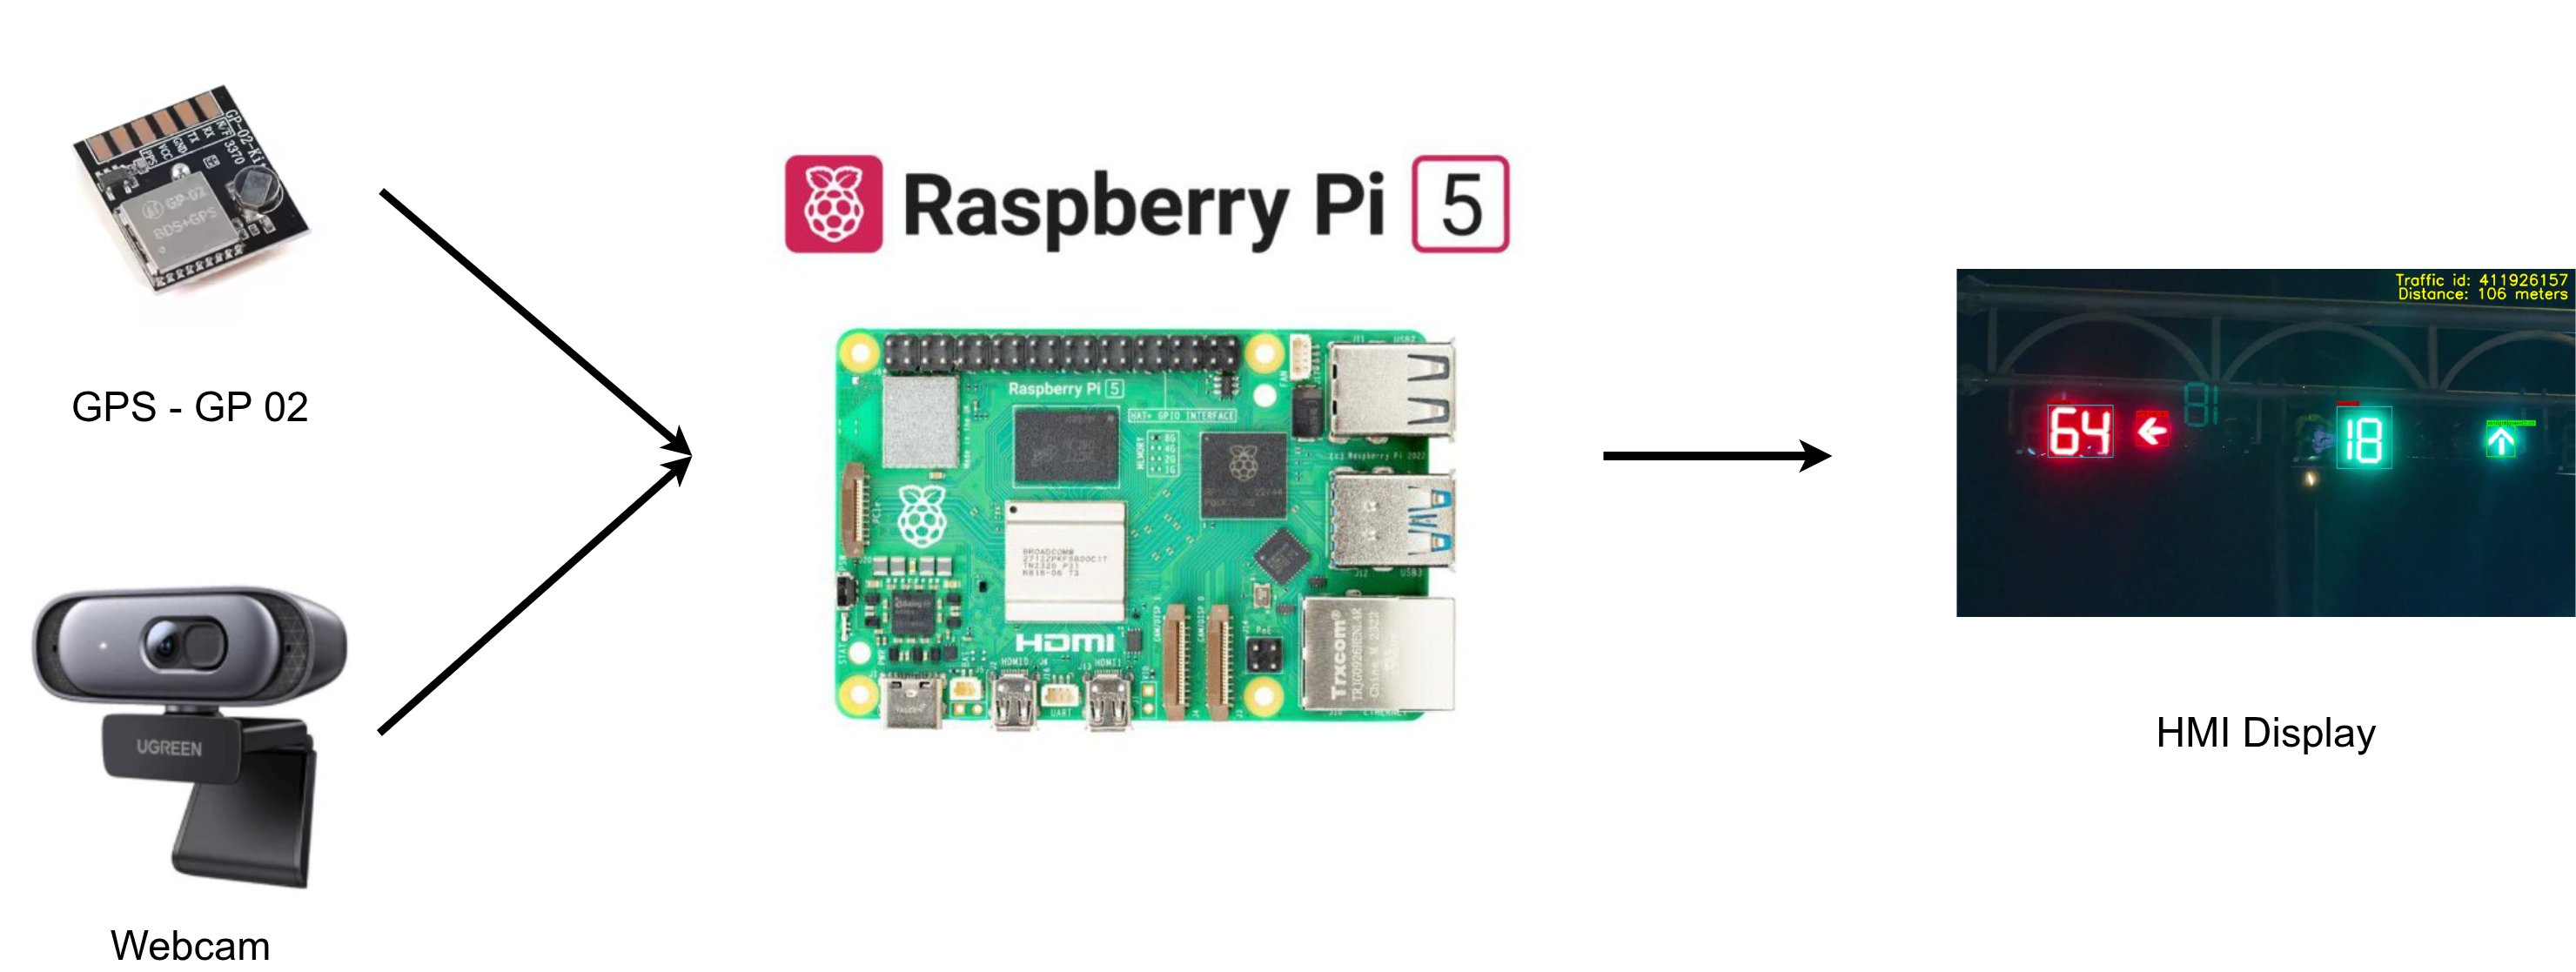
\includegraphics[width=0.8\textwidth]{Images/chapter2/hardware.png}
    \vspace{0.5cm}
    \caption{Hardware Architecture}
    \label{fig:hw_arch}
\end{figure}

\begin{itemize}
    \item \textbf{Raspberry Pi 5:} Acts as the central High-Performance Computing (HPC) unit, leveraging the Broadcom BCM2712 quad-core Arm Cortex-A76 processor clocked at 2.4GHz. This architecture delivers a \textbf{2-3x} performance boost over previous generations, providing the necessary computational overhead to execute complex Adaptive AUTOSAR applications, manage high-frequency DDS data distribution, and perform real-time edge-AI inference directly on the CPU.
    \item \textbf{USB Webcam:} Captures real-time video streams of the vehicle's surrounding environment, providing continuous visual input for the system's perception and object detection algorithms.
    \item \textbf{Ai-Thinker GP-02 GPS Module:} Acquires precise real-time geolocation data, including coordinates and velocity, which is essential for vehicle tracking and spatial awareness functions.
    \item \textbf{HMI Display:} Serves as the primary Human-Machine Interface, visually presenting critical information such as the real-time camera feed, object detection results, tracking data, and overall system status to the user.
\end{itemize}



In summary, the integration of Adaptive AUTOSAR, computer vision, AI inference via LiteRT, and GNSS-based spatial reasoning establishes the essential technical baseline for the proposed ADAS prototype. Rather than functioning as isolated technologies, the respective components form a coordinated ecosystem where software architecture, perception, localization, and physical hardware must seamlessly interact. Building upon that comprehensive background, the subsequent chapter transitions from theory to practical application. It details the exact configuration methodology, explaining how the selected frameworks are transformed into deployable AUTOSAR artifacts, trained AI models, and a reproducible execution environment.


% \input{}

